\documentclass[11pt,a4paper]{report}
\usepackage[T1]{fontenc}
\usepackage{amssymb}
\usepackage{amsthm}
\usepackage{natbib}
\usepackage{caption}
\usepackage{subcaption}
\usepackage{url}
\usepackage{amsmath}
\usepackage{hyperref}
\usepackage[utf8]{inputenc}
\renewcommand{\thesubfigure}{\thefigure\alph{subfigure}}
\usepackage{graphicx}
\graphicspath{ {./images/} }

\usepackage{pdflscape} %Landscape format

\renewcommand\thesection{\arabic{section}}
\renewcommand{\bibname}{Kaynakça}

\usepackage[ddmmyyyy]{datetime}
\renewcommand{\dateseparator}{.}


\renewcommand{\figurename}{Şekil}



\title{GÖRÜNTÜ İŞLEME İLE KALORİ HESAPLAMA-VİZE}

\author{Melisa Dursunoğulları}



\begin{document}
	\textbf{KÜTAHYA SAĞLIK BİLİMLERİ ÜNİVERSİTESİ}\\ \centering
	\textbf{MÜHENDİSLİK VE DOĞA BİLİMLERİ FAKÜLTESİ}\\ \centering
	\textbf{BİLGİSAYAR MÜHENDİSLİĞİ}\\ \centering
	\begin{figure}[!h]
		\centering
		
\includegraphics{ksbu}
		\maketitle
	\end{figure}
	\newpage
	
	
	\raggedright
	\section{Giriş}
	Son yıllarda yapay zeka ve görüntü işleme tekniklerindeki gelişmeler, birçok alanda önemli dönüşümlere neden olmuş ve hayatımızı her yönden etkileyip dahil olmuştur. Görüntü işleme, dijital görüntüler üzerinde bilgisayar algoritmaları ve matematiksel işlemler uygulayarak verileri analiz etmek ve anlamlı sonuçlar elde etmek için kullanılan bir bilgisayar bilimi dalıdır. Bu yöntemle bir görüntüdeki desenleri, nesneleri ve özellikleri tanımlamak, izlemek, sınıflandırmak ve ayıklamak için algoritmalar kullanılır.

    Görüntü işlemenin en temel amacı, görüntüdeki bilgiyi çıkarmak ve onu daha anlamlı bir formatta sunmaktır. Bu işlem sırasında görüntüdeki bilgi, piksellerin rengi, parlaklığı, kontrastı ve şekli gibi özellikleri kullanılarak matematiksel işlemlere tabi tutulur. İşte bu sayede görüntüdeki nesnelerin yerini, boyutlarını, şekillerini ve renklerini analiz etmek mümkün hale gelir\cite{SOCARTürkiye}.
    \newline

    Bu raporda görüntü işleme ile nesneleri tanımlayıp nesnenin durumu ve kalorisi hakkında bilgi edinebilme amaçlanmaktadır.Amaç görüntüyü analiz ederek şeklini, dokusunu,rengini hatta boyutuna bağlı olarak kalorisini hesaplayabilmektir.Özellikle kalori hesaplama, bireylerin günlük besin alımlarını izleyerek sağlıklı yaşam tarzlarını desteklemelerine yardımcı olacaktır. Görüntü işleme ve nesne tanıma teknikleri kullanılarak, yiyecek görüntülerinden kalori değerlerinin tahmin edilmesi, bireylere sağlıklı beslenme konusunda rehberlik sağlayacaktır.Ayrıca, bu raporda nesnelerin bozulmuş kısımlarının belirlenmesi ve işaretlenmesi gibi ek bilgiler içerecektir. Bu sayede ürünler hakkında daha detaylı bilgiler elde edilecek ve tüketicilere daha fazla bilgi sunulacaktır.Bu çalışmada, yapay zeka yöntemleri kullanılacaktır. Özellikle roboflow ile etiketleme yapılacak ve tensorflow,mediapipe ile opencv kütüphaneleri kullanılarak nesne tanıma ve kalori hesaplama işlemleri gerçekleştirilecektir. Bu tekniklerin bir araya getirilmesiyle, sağlıklı yaşam için önemli olan beslenme alışkanlıklarının takibi ve yönetimi kolaylaştırılacaktır.
    \newline

    Bu projenin kalbi "Detection" (algılama) yöntemidir. Projemizin odak noktası, YOLO (You Only Look Once) algoritması kullanılarak meyveleri algılama ve sınıflandırma yetenekleri üzerinedir. YOLO, yüksek doğruluk ve hızlı algılama süreleri ile tanınan bir nesne algılama algoritmasıdır.Günümüzde, görüntü işleme ve derin öğrenme tekniklerinin hızla gelişmesiyle birlikte, nesne algılama (object detection), nesne bölümleme (object segmentation), vücut pozunu tahmini (pose estimation) ve nesne sınıflandırması (classification) gibi alanlarda büyük ilerlemeler kaydedilmiştir. Bu teknikler, geniş bir uygulama yelpazesine sahiptir ve endüstriyel çözümlerde yaygın olarak kullanılmaktadır.
    \newline

    Bu projede, YOLO algoritması kullanılarak meyveleri algılama ve sınıflandırma yetenekleri geliştirilecektir. Projemizin ilerleyen bölümlerinde, projenin teknik ayrıntıları, kullanılan veri setleri, eğitim süreçleri ve elde edilen sonuçlar ele alınacaktır. Bu inceleme, projenin meyve algılama ve sınıflandırma yeteneklerini anlamamıza olanak sağlayacaktır.

    Raporun devamında ele alınacak konular arasında nesne algılama (object detection), nesne bölümleme (object segmentation), vücut pozunu tahmini (pose estimation) ve nesne sınıflandırması (classification) gibi temel derin öğrenme teknikleri yer alacaktır. Bu tekniklerin ne olduğu, nasıl çalıştığı ve amaçları incelenecek ve açıklanacaktır.
    \newline

    Nesne algılama teknikleri ve özellikle YOLO gibi hızlı ve etkili algoritmaların kullanımı, meyve tanıma ve sınıflandırma gibi uygulamalarda büyük potansiyele sahiptir. Bu teknolojilerin yaygınlaşmasıyla birlikte, iş süreçlerinin daha akıllı, verimli ve doğru bir şekilde yönetilebileceği görülmektedir. Bu rapor, nesne algılama ve derin öğrenme tekniklerine ilişkin temel bilgileri sunarak, projemizin önemini ve potansiyelini vurgulamaktadır.
    Projemizin temel amaçlarından biri de Webcam kamerasına bağlanarak gerçek zamanlı görüntü işleme tekniklerini kullanarak çeşitli nesneleri tanımaktır. Gelişmiş yapay zeka teknikleriyle donatılmış olan YOLO algoritması, bu projede nesnelerin tespit edilmesi ve sınıflandırılmasında temel araç olacaktır.
    Bu projede kalori belirlenebilmesinin ana şartı kameradan alınan görüntünün gerçek boyutunu belirleyebilmektir.Gerçek boyut için bir referans nesne kullanılmıştır. Bu referans nesne, kalibrasyon adımında kullanılarak görüntüdeki diğer nesnelerin boyutlarının hesaplanmasında temel bir ölçüt olarak görev almıştır.
    \newline

    Bu kalibrasyon referans nesnesinin seçiminde iki önemli özellik dikkate alınmıştır:
    \begin{itemize}
	   \item Özellik 1: Nesnenin ölçülerini (genişlik veya yükseklik cinsinden) ölçülebilir bir birim (milimetre, inç vb.) cinsinden bilinmesi.
	   \item Özellik 2: Bu referans nesnesini bir görüntüde, nesnenin yerleşimine bağlı olarak (referans nesnesinin  her zaman görüntünün sol üst köşesine yerleştirilmesi gibi) veya görünümler aracılığıyla (örneğin, kendine özgü bir renk veya şekil olması, benzersiz ve görüntüdeki diğer tüm nesnelerden farklı olması)tanılanabilir olmalı. Her iki durumda da referansımız bir şekilde benzersiz bir şekilde tanımlanabilir olmalıdır.\footnote{Bu projede ilk A4 kağıdı referans olarak alınmış sonrasında el ve parmak ucu referans alınmıştır.}\newline
	   
    \end{itemize}
    
    
	Meyve ve sebzelerin gerçek boyutlarının belirlenebilmesi için el ve tırnak boyutunu referans alınacaktır. Kameradan alınan görüntülerle el ve tırnak boyutları ölçülerek meyvelerin gerçek boyutları hesaplanacaktır.
	Kameradan alınan görüntülerle elin boyutları ölçülecek, genişlik ve uzunluk noktaların ölçüleri kaydedilecektir. Parmak ucu boyutları, işaret, orta, yüzük, serçe ve küçük parmakların ayrı ayrı ölçülecektir. Her bir parmak için belirlenecektir.\newline
	
	Mediapipe ve OpenCV gibi görüntü işleme kütüphaneleri kullanılarak, kameradan alınan görüntülerde el ve parmak ucu tanımlanacaktır. Bu adımda, elin genel yapısı ve konumu tespit edilecektir.El ve parmak ucu boyutları piksel cinsinden ölçüldükten sonra, kameranın sabit bir uzaklığına göre gerçek dünya ölçülerine dönüştürülecektir.El ve parmak ucu boyutları referans alınarak, meyve ve sebzelerin görüntülerinde el ile karşılaştırma yapılacaktır.El veparmak ucu boyutlarına göre meyve ve sebzelerin gerçek boyutları hesaplanacaktır.
	\newline
	
	Bu projenin amacı, oluturulan bir veri seti üzerinde yapay zeka teknikleri ile bir nesnenin tespitini, boyutunu algılama,kalorisini hesaplama ve nesnenin durumunun tespit edilmesini gerçekleştirmektir.Bu projede kullanılan veri seti hazır değildir, özel olarak tek tek toplanmış ve etiketlenmiş bir veri setidir.


     
     \section{Yolo Algoritması Nedir?}
    YOLO (You only look once) türkçe karşılığı ‘Yalnızca bir kez bak ‘ olan , gerçek zamanlı nesne takibi için CNN (Convolutional Neural Network -Evrişimli Sinir Ağı) kullanan en yaygın algoritmadır.Gerçek zamanlı nesne takibi için RCNN (Regions with Convolutional Neural Networks), Fast R CNN (daha hızlı ve daha verimli) , Faster R CNN (daha hızlı daha doğru sonuç- nesne tespiti ve bölge önerisi (region proposal) aşamalarını tek bir ağ içinde birleştirir.) gibi uygulamalar 2015 yılında YOLO piyasaya sürülene kadar kullanılan popüler uygulamalardı. YOLO’yu diğer uygulamalardan ayıran en önemli özelliği çok hızlı olmasıdır. YOLO’nun çalışma mekanizmasına bakıldığında diğer nesne algılama yöntemlerinden farklı ve hızlı kılan birçok yönü bulunmaktadır. 
    \newline
    
    YOLO,görseli tek seferde bir sinir ağından geçirerek resimdeki nesnelerin koordinatlarını ve sınıfını tahmin eder. Bu, ağın bir resmi tek bir geçişte tarayarak ağır hesaplamalara gerek kalmadan nesneleri tespit edebilmesini sağlar. Bu tanımlamayı yaparken görseli 3*3 , 4*4,19*19 ızgaralara (grids) ayırır. Izgaraların sayısını belirlemek için belirli bir koşul yoktur. N*N formatında olması yeterlidir .Her ızgara kendi içerisinde nesne olup olmadığını ve nesne var olduğunu düşünüyorsa merkez noktasının kendi alanında olup olmadığını düşünür. Resim sinir ağından geçtikten sonra çıktı olarak bir vektör meydana gelir.\cite{mediumcom}
    
    \begin{figure}[!h]
    	\centering
    	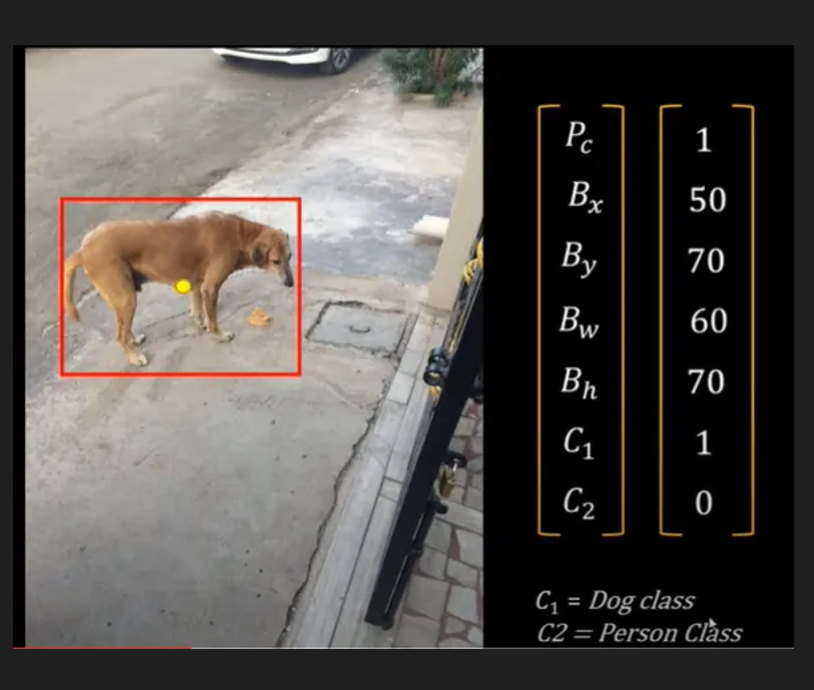
\includegraphics[width=0.75\textwidth]{matris}
    	\caption{Photo on Codebasics Youtube Channel by Dhaval Pate}
    	\label{fig:ornek}
    \end{figure}
    Şekil \ref{fig:ornek}'de görüldüğü gibi bir nesne için bir vektör meydana gelmektedir.
    
    
    \begin{itemize}
    	\item Pc (Probability of class): Sınıf olasılığıdır. Burada nesnenin yer alıp almamasına göre değerlendirme yapılır. Nesne olma olasılığı 1 ile , nesne olmama olasılığı 0 ile belli edilir. Bu görselde çerçevenin içerisinde köpek olduğu için Pc değeri 1'dir.
    	
    	\item  Bx: Köpeğin merkez noktasının (sarı nokta ile gösterilmiştir) x koordinatıdır.
    	
    	\item  By: Köpeğin merkez noktasının (sarı nokta ile gösterilmiştir) y koordinatıdır.
    	
    	\item  Bw: Kırmızı çerçevenin enidir .(Nesnenin eni, buradaki nesne köpektir.)
    	
    	\item Bh: Kırmızı çerçevenin yüksekliğidir. (Nesnenin yüksekliğidir, buradaki nesne köpektir.)
    	
    	\item  C1: Köpek sınıfını ifade eder.
    	
    	\item  C2: İnsan sınıfını ifade eder.
    	
    \end{itemize}
    
    Nesne tespitine iki ana yaklaşım vardır:
    \begin{itemize}
    	\item  İki aşamalı dedektörler Daha Hızlı R-CNN gibi, önce bölge önerileri üretir, ardından her bölgenin sınırlarını sınıflandırır ve hassaslaştırır. Daha doğru olma eğilimindedirler ancak daha yavaştırlar.
    	\item  Tek aşamalı dedektörler YOLO gibi, tek geçişte doğrudan görüntünün üzerine bir model uygulayın. Çok hızlı çıkarım süreleri için doğruluktan ödün veriyorlar.
    \end{itemize}
    
    \begin{figure}[!h]
    	\centering
    	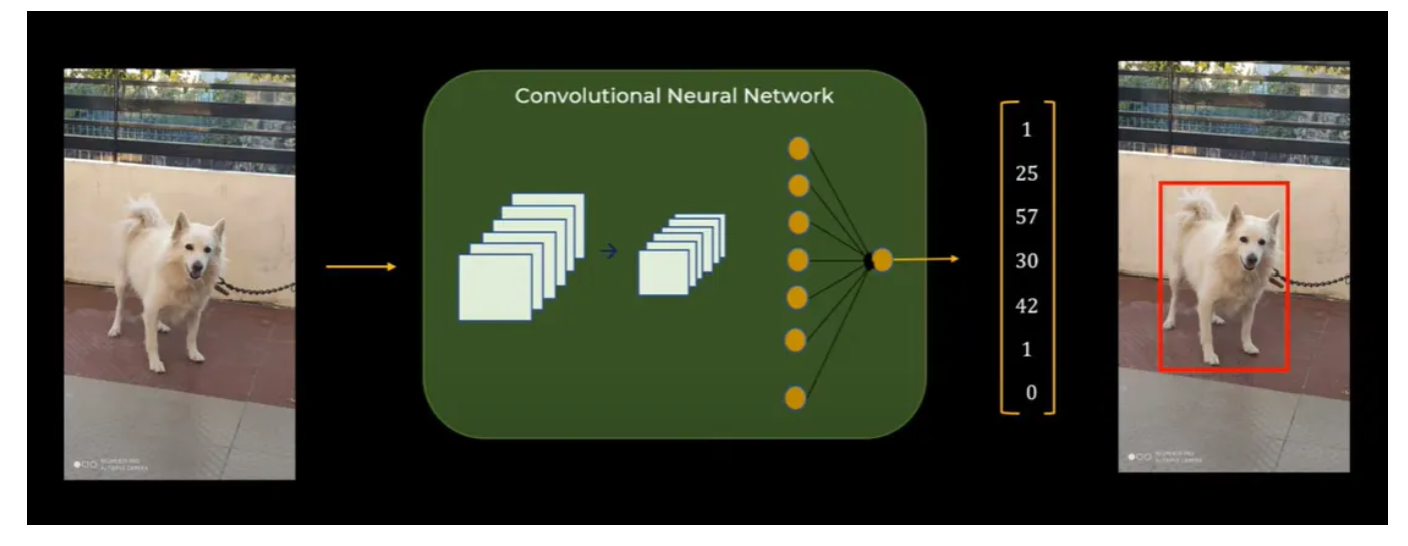
\includegraphics[width=\textwidth]{yolo}
    	\caption{Photo on Codebasics Youtube Channel by Dhaval Pate}
    	\label{fig:ornek2}
    \end{figure}
    \newpage
    
    \begin{figure}[!h]
    	\centering
    	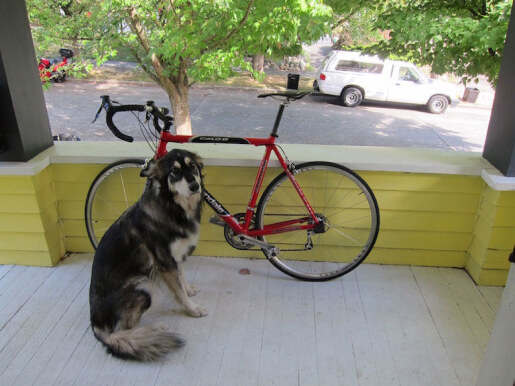
\includegraphics[width=\textwidth]{nesnetanıma1}
    	\caption{Nesne tanıma işlemi yapılacak fotoğraf}
    	\label{fig:ornek3}
    \end{figure}
    
    Şekil \ref{fig:ornek3}'deki resime YOLO ile nesne tanıma yaptırılacaktır. 
    
    
    \begin{figure}[!h]
    	\centering
    	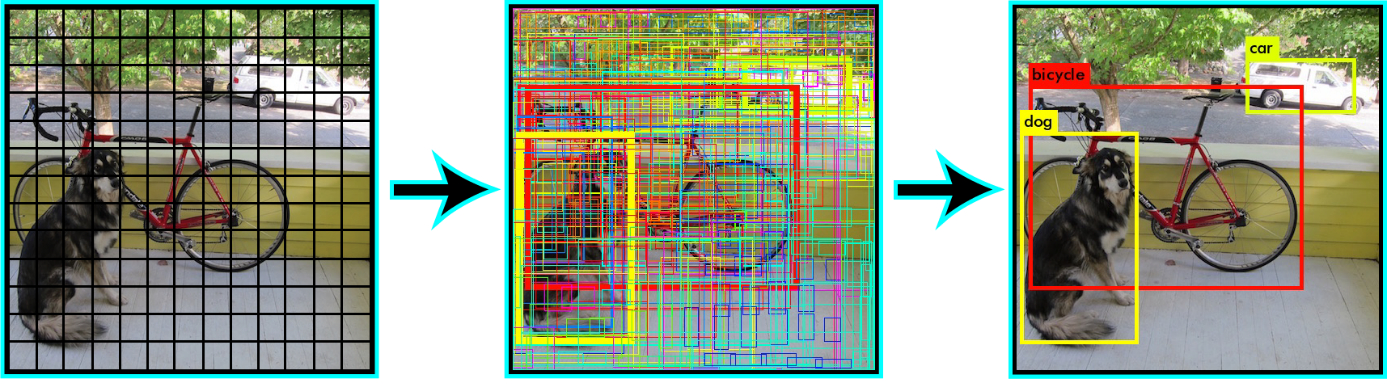
\includegraphics[ width=1.30\textwidth]{nesne-tanıma2}
    	\label{ornek4}
    	\caption{detection işlemi yapılacak fotoğraf}
    \end{figure}
    İlk önce girdi resmini SxS‘lik ızgaralara bölüyor.Her bir ızgara kendi içinde, alanda nesnenin olup olmadığını, varsa orta noktasının içinde olup olmadığını, orta noktası da içindeyse uzunluğunu, yüksekliğini ve hangi sınıftan olduğunu bulmakla sorumlu. Resimde köpeğin orta noktasının olduğu ızgara köpeğin tespit edilmesinden/etrafına kutucuk çizmesinden sorumlu.
    \newline
    
    Buna göre YOLO her ızgara için ayrı bir tahmin vektörü oluşturur.Her bir ızgara sadece 1 tane nesne tanımlayabiliyor. \newline
    
    \textbf{Güven skoru:} Bu skor modelin geçerli ızgara içinde nesne bulunup bulunmadığından ne kadar emin olduğunu gösterir. (0 ise kesinlikle yok 1 ise kesinlikle var) Eğer nesne olduğunu düşünürse de bu nesnenin gerçekten o nesne olup olmadığından ve etrafındaki kutunun koordinatlarından ne kadar emin olduğunu gösterir.\cite{mediumcom2}
    \newline
    
    $ \text{Güven Skoru} = \text{Pr(obj)} \times \text{IoU} $
    \newline
    
    Pr(obj): ızgara içinde nesnenin bulunma olasılığı
    
    IoU: gerçekte nesnenin bulunduğu kutu ile tahmin edilen kutunun kesişimi
    \newline
    
    YOLO’nun çalışma mantığını özetlersek,
    \begin{itemize}
    	\item Algoritma görseli öncelikle ızgaralara ayırır.
    	
    	\item Her bir bölgedeki nesnelerin etrafına çerçeve (bounding box) çizer.
    	
    	\item Her bir bölgede nesne bulunma olasılığını hesaplar.
    	
    	\item Her bir çerçeve (bounding box) için güven skoru hesaplar.
    \end{itemize}
    Diğer geleneksel nesne algılama yöntemlerine kıyasla YOLO, oldukça hızlı ve gerçek zamanlı uygulamalarda etkili bir şekilde çalışabilir. Bu özelliği, özellikle canlı video akışı gibi anlık işlemlerde ve gerçek zamanlı uygulamalarda avantaj sağlar.
    
    
    \section{Nesne Algılama ve Sınıflandırma Veri Kümeleri}
    
    Bilgisayarlı görü, nesne tanıma, nesne algılama ve sınıflandırma gibi alanlarda büyük ölçüde gelişmiştir. Bu gelişmelerin bir kısmı, çeşitli veri kümeleri sayesinde gerçekleştirilmiştir. Bu veri kümeleri, derin öğrenme modellerinin eğitimi ve değerlendirmesi için temel oluşturur.
    \begin{itemize}
    	\item Detection (COCO)
    	
    	\item Detection (Open Image V7)
    	
    	\item Segmentation 
    	
    	\item Pose 
    	
    	\item OBB (DOTAv1)
    	\item Classification (ImageNet) 
    \end{itemize}
    \newpage
    
    \begin{figure}[!h]
    	\centering
    	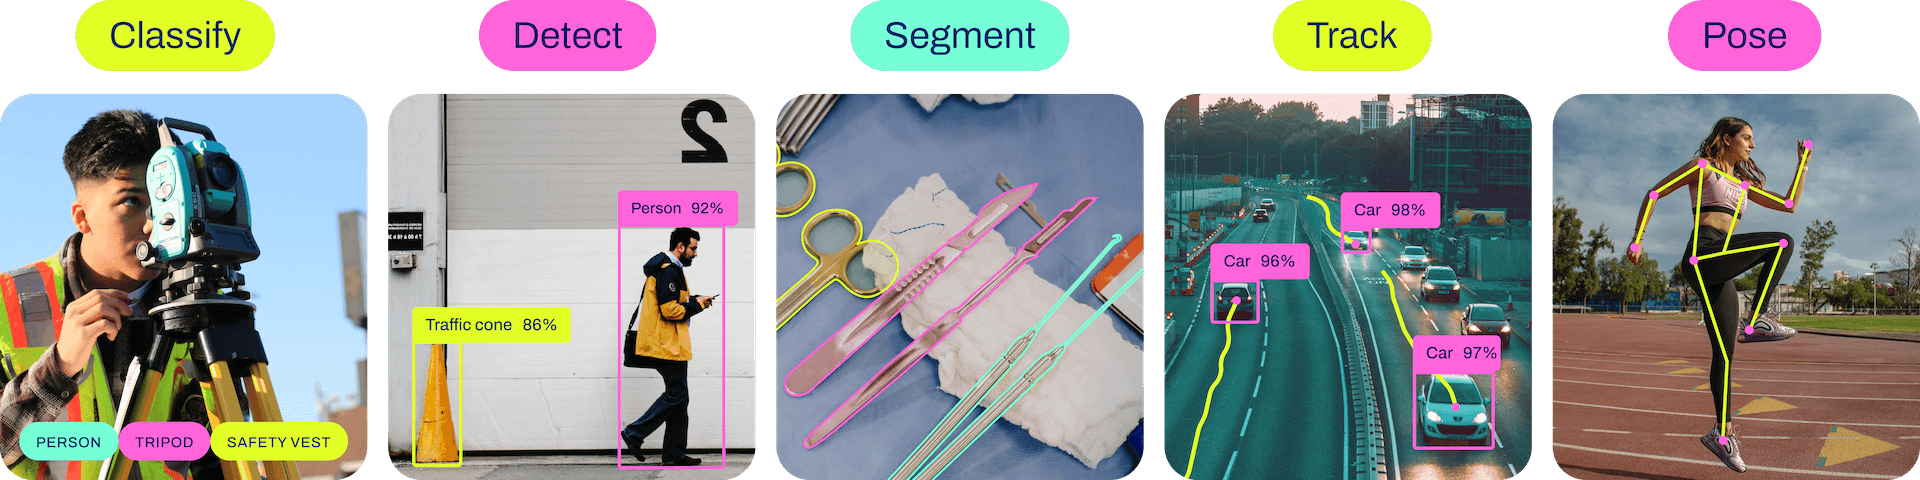
\includegraphics[width=\textwidth]{banner-tasks}
    	\caption{ultralytics}
    	\label{fig:ornek5}
    \end{figure}
    \subsection{Detection (COCO)}
    
    COCO, nesne tanıma, nesne tespiti ve nesne segmentasyonu için popüler bir veri kümesidir. İçinde 80 farklı nesne kategorisi barındırır ve her bir resimde bu nesnelerin detaylı etiketleri bulunur. Özellikle nesne segmentasyonu için ayrıntılı piksel bazında segmentasyon maskeleri sağlar.
    
    \subsection{Detection (Open Image V7)}
    
    Google tarafından sunulan büyük bir resim veri kümesidir. COCO'dan daha geniş bir etiket kategorisi yelpazesi sunar ve 9 milyondan fazla etiketlenmiş resme sahiptir. Sınırlayıcı kutular ve sınıf etiketleriyle nesne tespiti ve sınıflandırma görevlerinde kullanılır.Open Images, COCO gibi ayrıntılı piksel bazında segmentasyon maskeleri sağlamaz. Ancak nesnelerin sınırlayıcı kutuları ve sınıf etiketleri mevcuttur.
    \newline
    
    \textbf{ Farkları}
    \newline
    
    COCO, daha az etiket kategorisine sahip olmasına rağmen, nesne segmentasyonu için detaylı maske bilgileri sağlar.
    Open Images V7, çok daha geniş bir etiket kategorisi yelpazesi sunar ve çok daha fazla sayıda resme sahiptir.
    COCO'nun daha spesifik görevler için daha ayrıntılı veri sağladığı söylenebilirken, Open Images V7 daha genel ve çeşitli veri sağlar.
    Hangi veri kümesinin kullanılacağı, kullanım senaryosuna ve ihtiyaca bağlıdır. Örneğin, daha geniş bir nesne kategorisi yelpazesi gerekiyorsa Open Images V7 tercih edilebilirken, nesne segmentasyonu gibi piksel bazında ayrıntılı bilgiler gerekiyorsa COCO daha uygun olabilir.\cite{ultralytics}
    \newpage
    
    \subsection{Segmentation}
    
    Temelde, bir görüntüdeki nesnelerin veya bölümlerin (segmentlerin) belirlenmesi işlemidir. Bu işlem, görüntüdeki pikselleri farklı nesnelere veya bölümlere ayrılmış gruplara ayırarak gerçekleştirilir. Segmentasyon, nesne tanıma, nesne tespiti, nesne izleme, medikal görüntüleme ve daha birçok alanda kullanılır.
    
    \begin{figure}[!h]
    	\centering
    	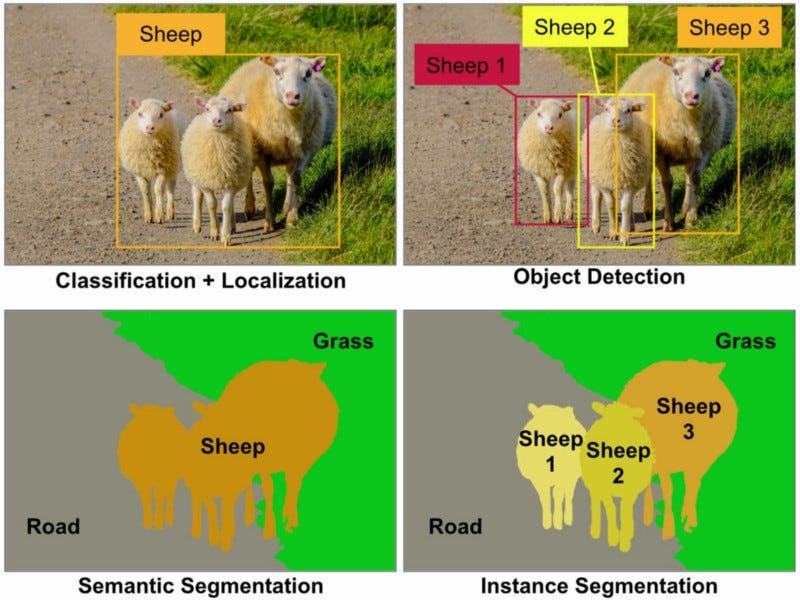
\includegraphics[width=\textwidth]{segmentation-1}
    	\caption{segmentation}
    	\label{fig:ornek6}
    \end{figure}
    
    \textbf{Semantic (Anlamsal) Segmentasyon:} "Semantic Segmentasyon" veya "Anlamsal Segmentasyon", bir görüntüdeki her bir pikselin ait olduğu nesne veya bölge sınıfını belirlemeyi amaçlayan bir görüntü işleme ve derin öğrenme görevidir. Temel amacı, görüntüdeki her pikseli, o pikselin ait olduğu nesne veya bölgenin genel sınıfına atamaktır. Bu yöntem, pikselleri ayrı ayrı nesnelere veya bölümlere sınıflandırarak görüntüyü anlamlandırmayı hedefler.
    \newline
    
    \textbf{Instance Segmentation:}nesne algılama ve nesne segmentasyonu yöntemlerinin bir kombinasyonudur.Bu yöntem, bir görüntüdeki her bir nesneyi ayrı tanımlamayı ve sınıflandırmayı, aynı zamanda her bir nesnenin piksel bazında segmentasyonunu gerçekleştirmeyi amaçlar. Yani, görüntüdeki her bir nesneyi belirlerken, nesnelerin sınırlarını (bounding box) çizerken aynı zamanda her bir nesnenin piksellerini de ayrı tanımlar.
    
    \section{Classification}
    
    "Classification" (Sınıflandırma), makine öğrenimi ve derin öğrenme alanlarında önemli bir konsepttir. Temelde, bir girdiyi belirli bir kategoriye veya sınıfa atama işlemidir. Bu işlem genellikle önceden belirlenmiş bir sınıf listesinden birine karar vermek için yapılır. Örneğin, bir resmi "köpek", "kedi", "araba" gibi belirli bir kategoriye sınıflandırmak gibi.\cite{Segmentasyon}
    
    \begin{figure}[!h]
    	\centering
    	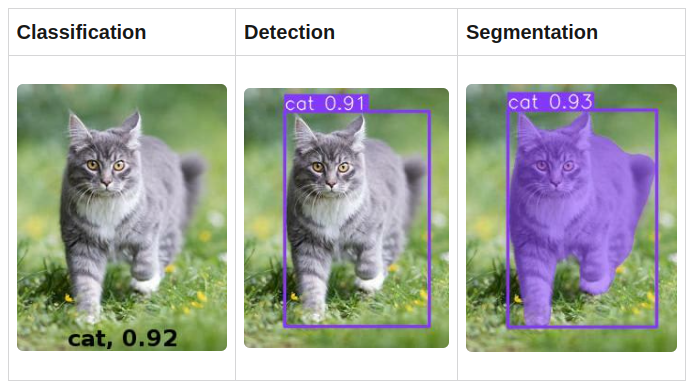
\includegraphics[width=\textwidth]{compvision}
    	\caption{segmentation}
    	\label{fig:ornek7}
    \end{figure}
    
    \section{Sınıflandırma Projesi}
    
    Bu projede, YOLO (You Only Look Once) nesne algılama algoritmasının farklı meyveleri tanıma ve sınıflandırma yeteneğini incelenmiştir. Özellikle, aynı renklere sahip meyvelerin birbirine benzetilip benzetilmediği ve YOLO'nun bu meyveleri nasıl sınıflandırdığına odaklanılmıştır.
    
    Hazırlanan veri seti üzerinde YOLOv8 algoritması kullanılarak bir nesne algılama modeli eğitilmiştir. Eğitim sürecinde 70 epoch (dönem) ve imgsz=640 (çözünürlük) kullanıldı.
    
    İlk olarak, aynı renklere sahip meyvelerin birbirine benzetilip benzetilmediği test edilmiştir. Özellikle, farklı renklerdeki elma örneklerini ve sarı renkteki muz ve limon gibi meyveleri sınıflandırma yeteneği test edilmiştir. Model, genel olarak bu meyveleri sınıflandırmada ortalama bir başarı elde etti. Ancak bazı dikkate değer durumlar mevcuttur:
    \clearpage
    
    
    
    \begin{figure}[!h]
    	\begin{subfigure}{\textwidth}
    		\centering
    		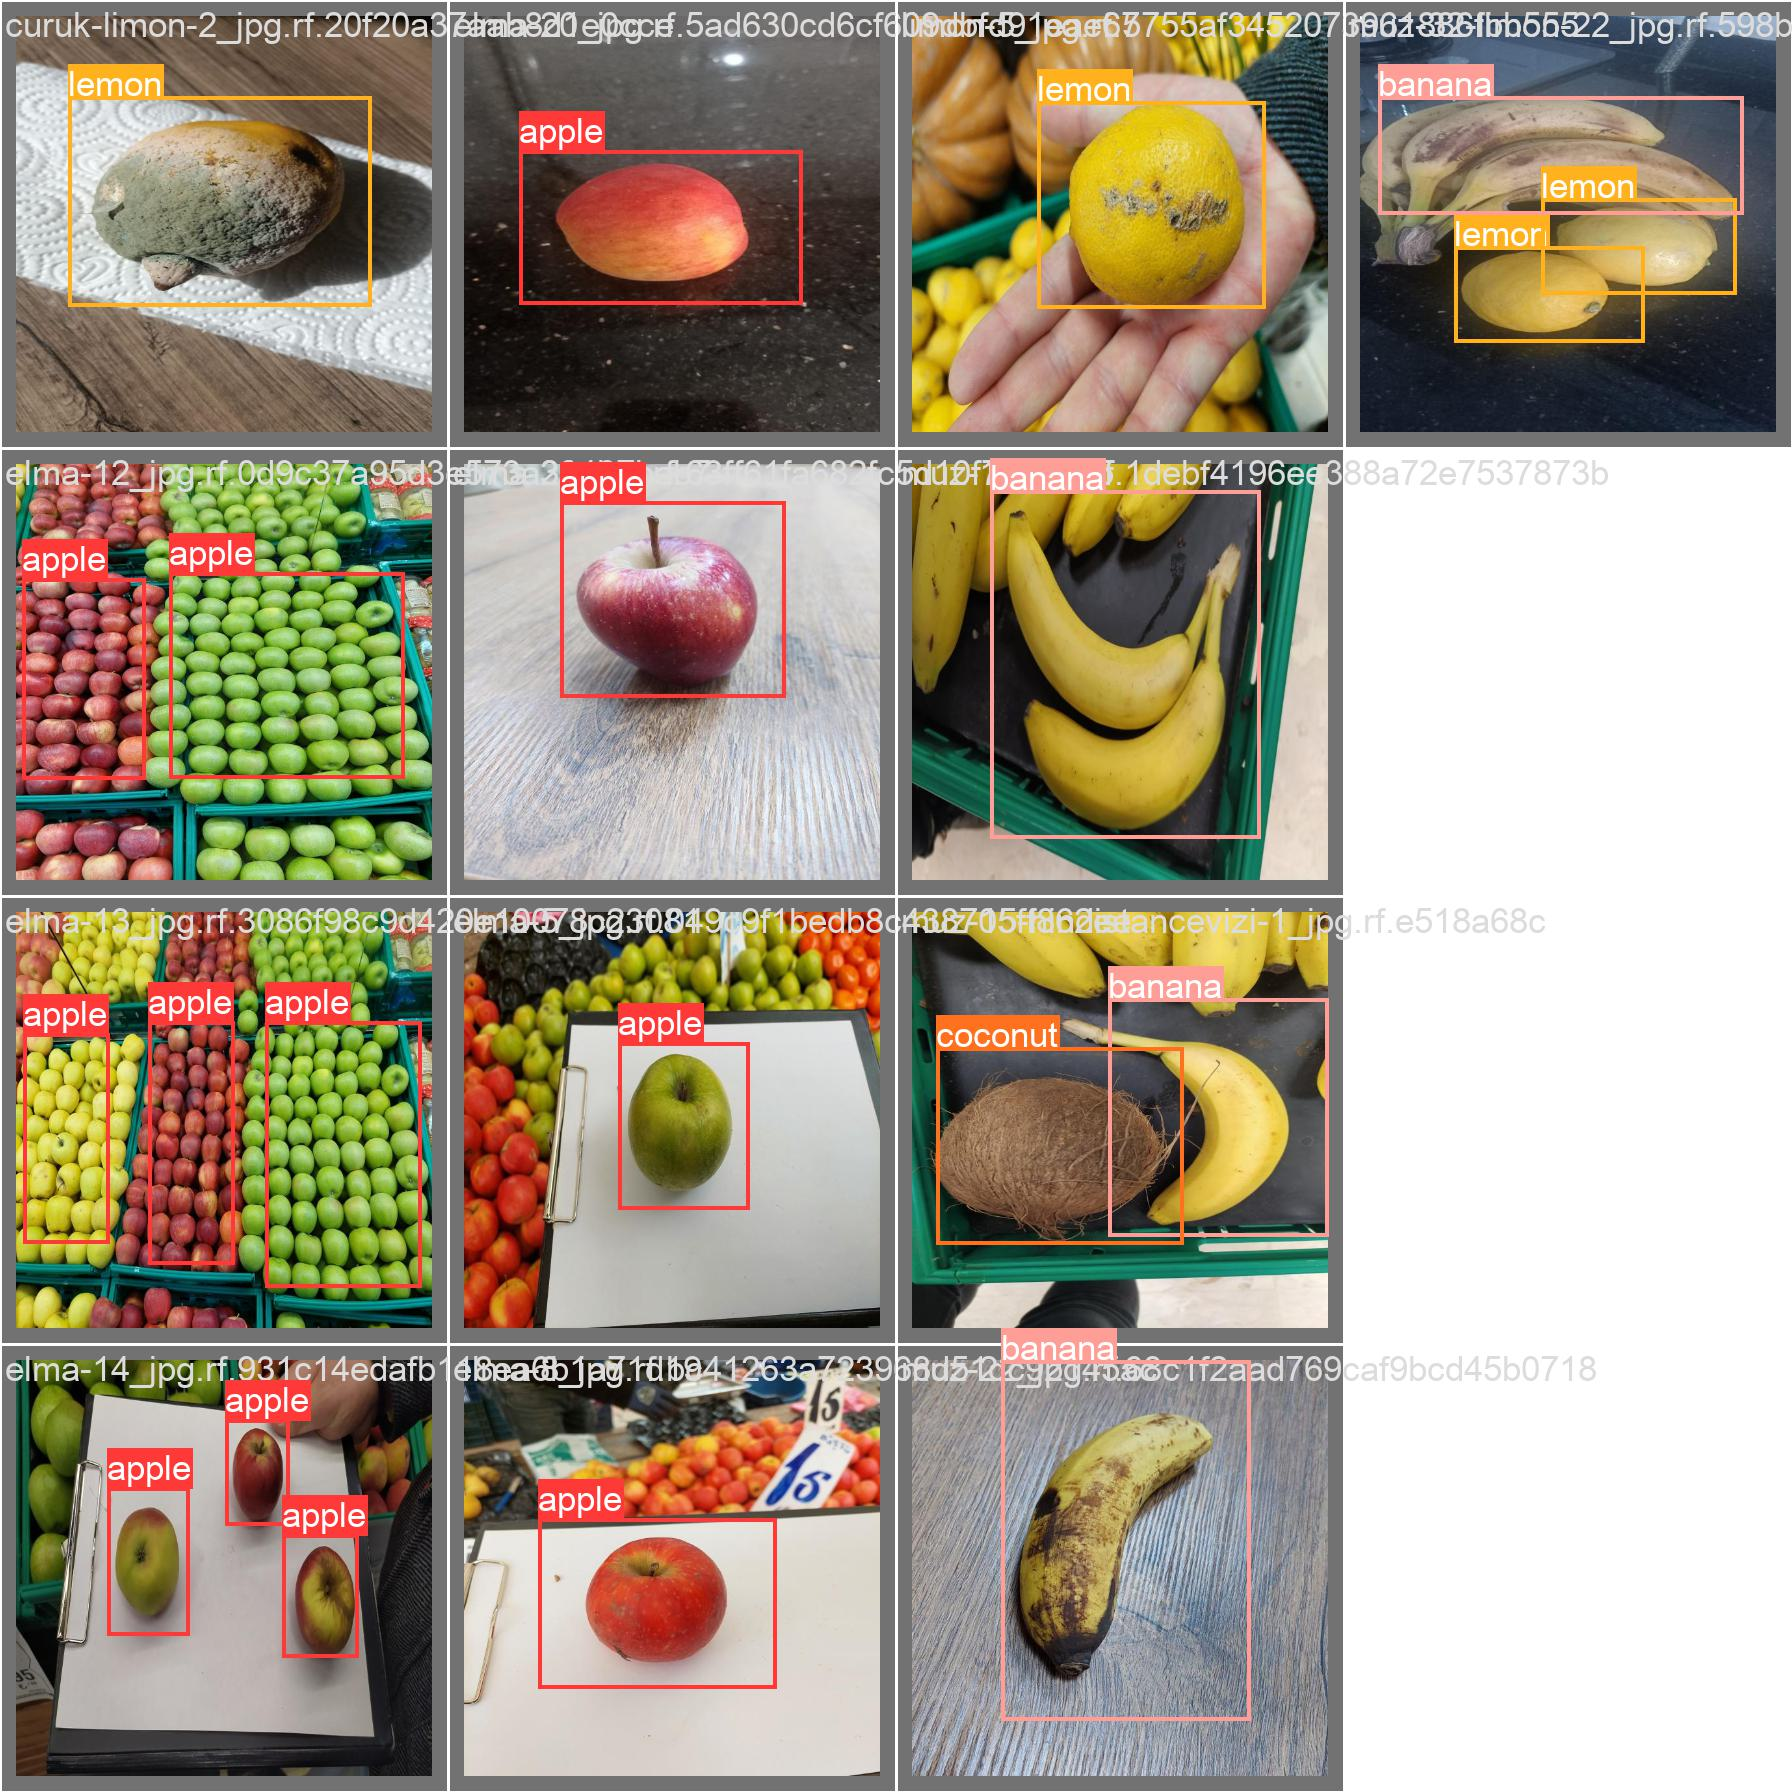
\includegraphics[width=0.8\linewidth]{örnek1}
    		\caption{Nesne Tespiti}
    		\label{fig:ornek8}
    	\end{subfigure}
    	
    	\begin{subfigure}{\textwidth}
    		\centering
    		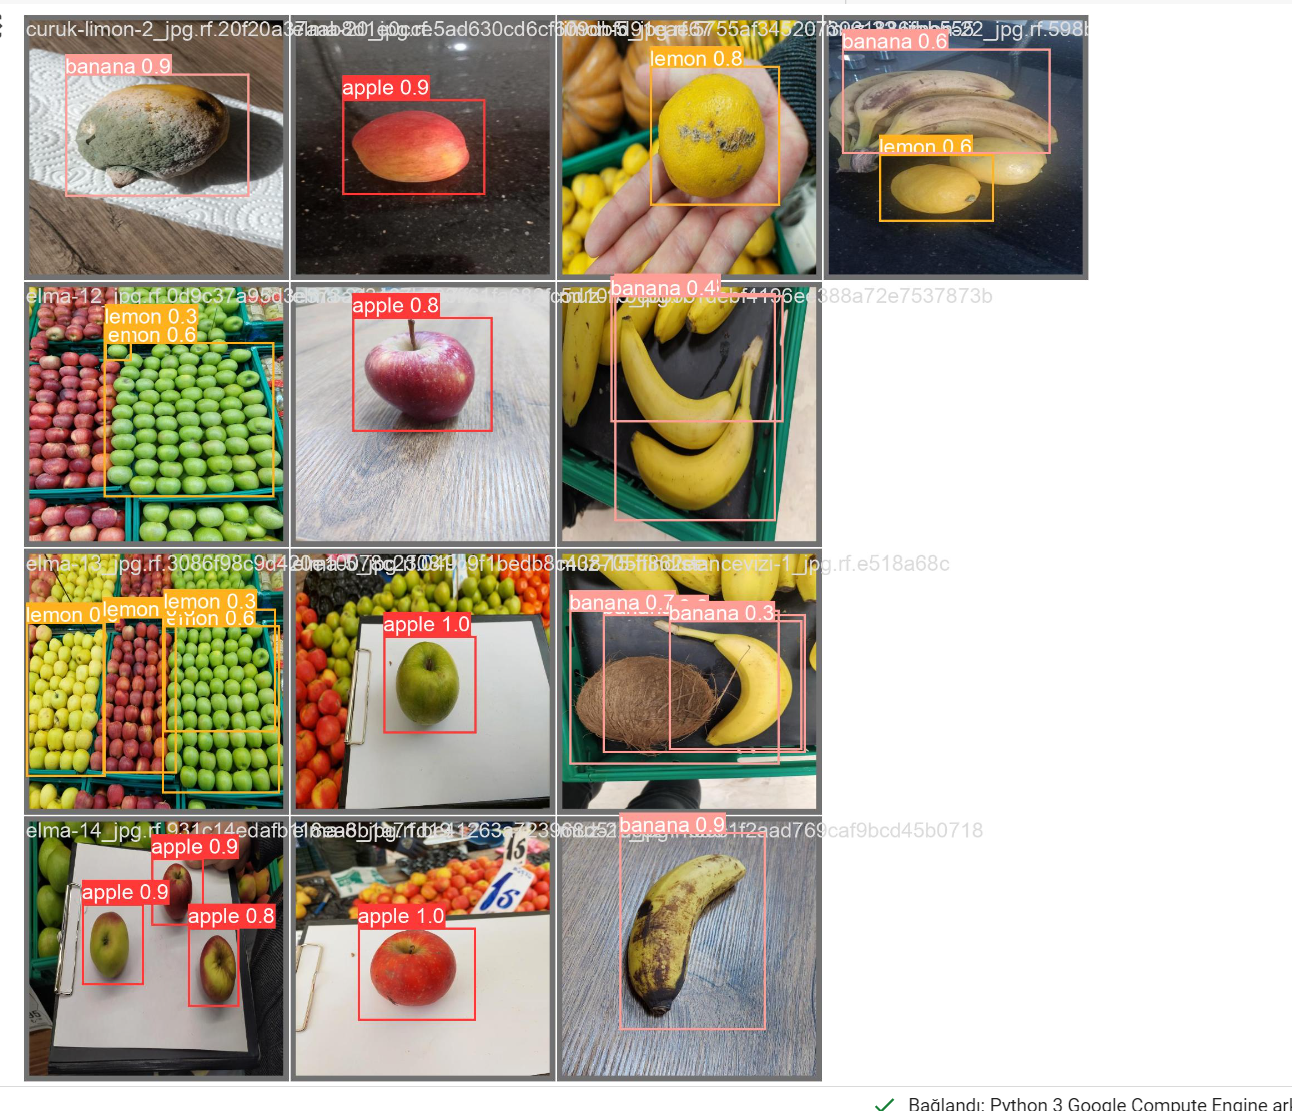
\includegraphics[width=0.8\linewidth]{örnek2}
    		\caption{Nesne tespiti ile Güven Skoru}
    		\label{fig:ornek9}
    	\end{subfigure}
    	
    	
    \end{figure}
    
    \textbf{Elma Sınıflandırması:} Model, farklı renklerdeki elma örneklerini genellikle doğru şekilde sınıflandıramadı. Kırmızı, yeşil ve sarı gibi farklı renklere sahip elmalara çoğunlukla doğru etiketler verilemedi.Model, bazı sarı renkli elma örneklerini limon olarak etiketledi. Bu durum, modelin renk bazında sınıflandırma yeteneğinde belirli bir hassasiyetsizlik olduğunu gösteriyor.
    \newline
    
    \textbf{Muz ve Limon Sınıflandırması:} Sarı renkteki muz ve limon gibi meyveleri ayırt etme konusunda genel olarak iyi bir performans sergilemiştir. Model, muz ve limonları doğru şekilde sınıflandırdı ve genellikle bu meyveleri ayırt etmiştir. Ancak bazı durumlarda, özellikle çürük veya hasarlı limonların tanınmasında zorlanma yaşandı. Model, çürük limonları genellikle muz olarak sınıflandırdı.	

		\subsection{Nesne Tanıma ve Sınıflandırma}
	Projemizin ana amacı, kameradan anlık görüntü alarak bu görüntüde bulunan nesneleri tespit etmek ve sınıflandırmaktır. Örneğin, araba, insan, bisiklet gibi nesneleri belirlemek ve bu nesnelerin hangi sınıfa ait olduğunu tespit etmek projenin temel hedefidir.
	\subsection{Gerçek Zamanlı Uygulama} 
	Bu proje gerçek zamanlı uygulamayı hedeflemektedir. Yani, kamera görüntüsünden aldığımız her bir karede nesneleri tanımlayacak ve sınıflandıracak bir sistem geliştireceğiz. Bu, kullanıcıya anlık olarak nesnelerin tespit edilip sınıflandırılmasını sunacak bir uygulama anlamına gelmektedir.
	\subsection{ Hızlı ve Doğru Tanıma}
	YOLO algoritması, hızlı çalışma ve yüksek doğruluk gibi avantajlarıyla öne çıkar. Bu proje, YOLO'nun bu özelliklerinden faydalanarak gerçek zamanlı nesne tanıma işlemini başarıyla gerçekleştirmeyi amaçlamaktadır. Kullanıcıya hızlı ve doğru nesne tanımlama deneyimi sunmayı hedeflemekteyiz.
	\newpage
	
	\section{OpenCV Nedir?}
	OpenCV (Open Source Computer Vision) açık kaynak kodlu görüntü işleme kütüphanesidir.OpenCV platform bağımsız bir kütüphanedir, bu sayede Windows, Linux, FreeBSD, Android, Mac OS ve iOS platformlarında çalışabilmektedirOpenCV kütüphanesi içerisinde görüntü işlemeye (image processing) ve makine öğrenmesine (machine learning) yönelik 2500’den fazla algoritma bulunmaktadır. Bu algoritmalar ile yüz tanıma, nesneleri ayırt etme, insan hareketlerini tespit edebilme, nesne sınıflandırma, plaka tanıma, üç boyutlu görüntü üzerinde işlem yapabilme, görüntü karşılaştırma, optik karakter tanımlama OCR (Optical Character Recognition)	gibi işlemler rahatlıkla yapılabilmektedir. OpenCV geniş bir kaynağa sahiptir, yapmak istediğiniz şeyle alakalı olarak size yardımcı olacak topluluklar ve bulabileceğiniz teknik dokumanlar oldukça fazladır. Bilişim sektöründe kullanım oranı fazla olan bütün programlama dillerine desteği bulunmaktadır, açık kaynak kodlu olması itibari ile de doğrudan desteği bulunmayan programlama dilleri için ara katmanlar yazılmış ve OpenCV bu dile entegre edilmiştir.\cite{picskin2016opencv}
	
	\section{OpenCV Projeleri}
	\subsection{Webcam Bağlantı Projesi}
	Webcam'e bağlanarak gerçek zamanlı görüntü almak, nesne tanıma projemizin ilk adımıdır. Bu adımda, Spyder IDE'si kullanılarak Webcam'e bağlanma işlemi gerçekleştirilecektir.Webcam'den alınan görüntüleri daha sonra nesne tanıma algoritmalarıyla işlenecektir.
	
	OpenCV (Açık Kaynak Bilgisayar Görüntü İşleme Kütüphanesi): Webcam'e bağlanmak ve görüntü işlemek için kullanılacak olan temel kütüphanedir.
	
	\newpage
	
	\begin{figure}[!h]
		\centering
		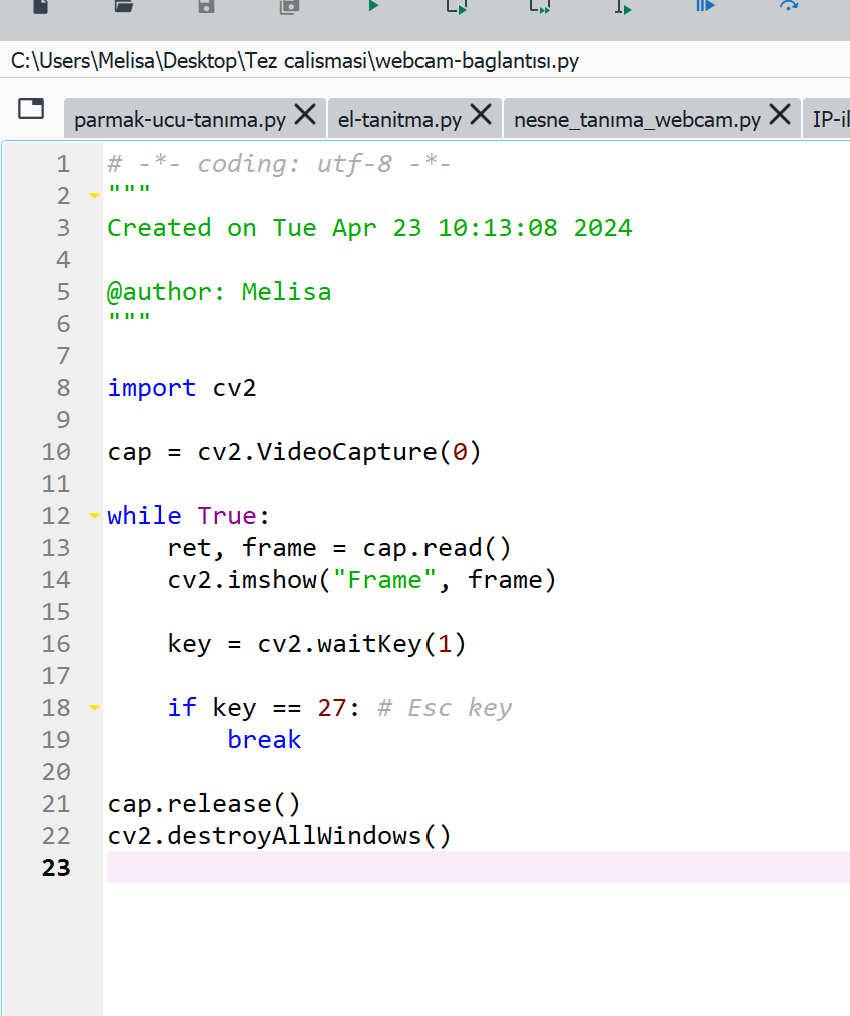
\includegraphics[width=0.75\textwidth]{webcam-baglantisi}
		\caption{Webcam Bağlantısı}
		\label{fig:ornek1}
	\end{figure}
	Şekil-\ref{fig:ornek1} de webcam bağlantısın için python kodu gösterilmiştir.
	\newline
	
	Yukarıdaki kod (şekil-\ref{fig:ornek1}), Webcam'e bağlanarak kameradan alınan görüntüyü ekranda göstermektedir. Kodun adımları şu şekildedir:
	\begin{itemize}
		\item cv2.VideoCapture(0): Bu satır, 0 parametresiyle bir VideoCapture nesnesi oluşturarak Webcam'e bağlanır.
		
		\item cap.read(): Bu satır, Webcam'den bir kare alır ve bu kareyi frame değişkenine atar.Okuma işlemi yapılır.
		
		\item cv2.imshow('Webcam', frame): Bu satır, frame içeriğini 'Webcam' adıyla bir pencerede gösterir.
		
		\item  cv2.waitKey(1) \& 0xFF == ord('q'): Bu satır, 'q' tuşuna basıldığında döngüyü sonlandırır.
		
		\item cap.release() ve cv2.destroyAllWindows(): Bu satırlar, kullanım sona erdiğinde kamerayı serbest bırakır ve açık olan pencereleri kapatır.
	\end{itemize}
	\newpage
	
	\subsection{Webcam ile Telefon Bağlantısı Kurma Projesi}
	Telefona yüklenen 'IP WEBCAM' uygulaması ile ip adresi sayesinde webcam ve telefon rahatlıkla bağlantı kurabilmektedir.
	Telefonu bir IP Webcam olarak kullanmak için "IP Webcam" uygulaması kullanılacaktır.Bu uygulama, telefonun kamerasını bir IP adresi üzerinden erişilebilir hale getirir ve bu şekilde bilgisayara bağlanarak Webcam olarak kullanılır.
	
	\begin{itemize}
		\item İlk olarak, Android telefonun Google Play Store'undan "IP Webcam" uygulaması indirilir.
		
		\item Uygulama açıldıktan sonra, kullanmak istenen kamera, video çözünürlüğü, port numarası gibi ayarlar yapılabilir.Bu ayarlar IP adresi oluşturulduğunda önemli olacaktır.
		
		
		\item IP Webcam uygulaması açıldığında, uygulama bir IP adresi verecektir. Bu IP adresi, telefonun kamerasına erişim sağlayan adresdir.Örneğin, "http://192.168.1.101:8080" gibi bir IP adresi olabilir.
		
		\item IP Webcam uygulamasında belirlenen bağlantı portu (genellikle 8080 kullanılır) da önemlidir.
		
		
		\item Bilgisayarın web tarayıcısı ve telefonun IP adresi aynı olmalıdır. Örneğin, "http://192.168.1.101:8080" şeklinde olmalı.
		
		\item Bu adımları doğru şekilde uygulandıysa, tarayıcıda telefonun kamerasından canlı görüntü alınabilir.Bu, telefonun IP Webcam olarak kullanılması için gerekli bağlantıyı sağlar.
	\end{itemize}
	
	\begin{figure}[!h]
		\centering
		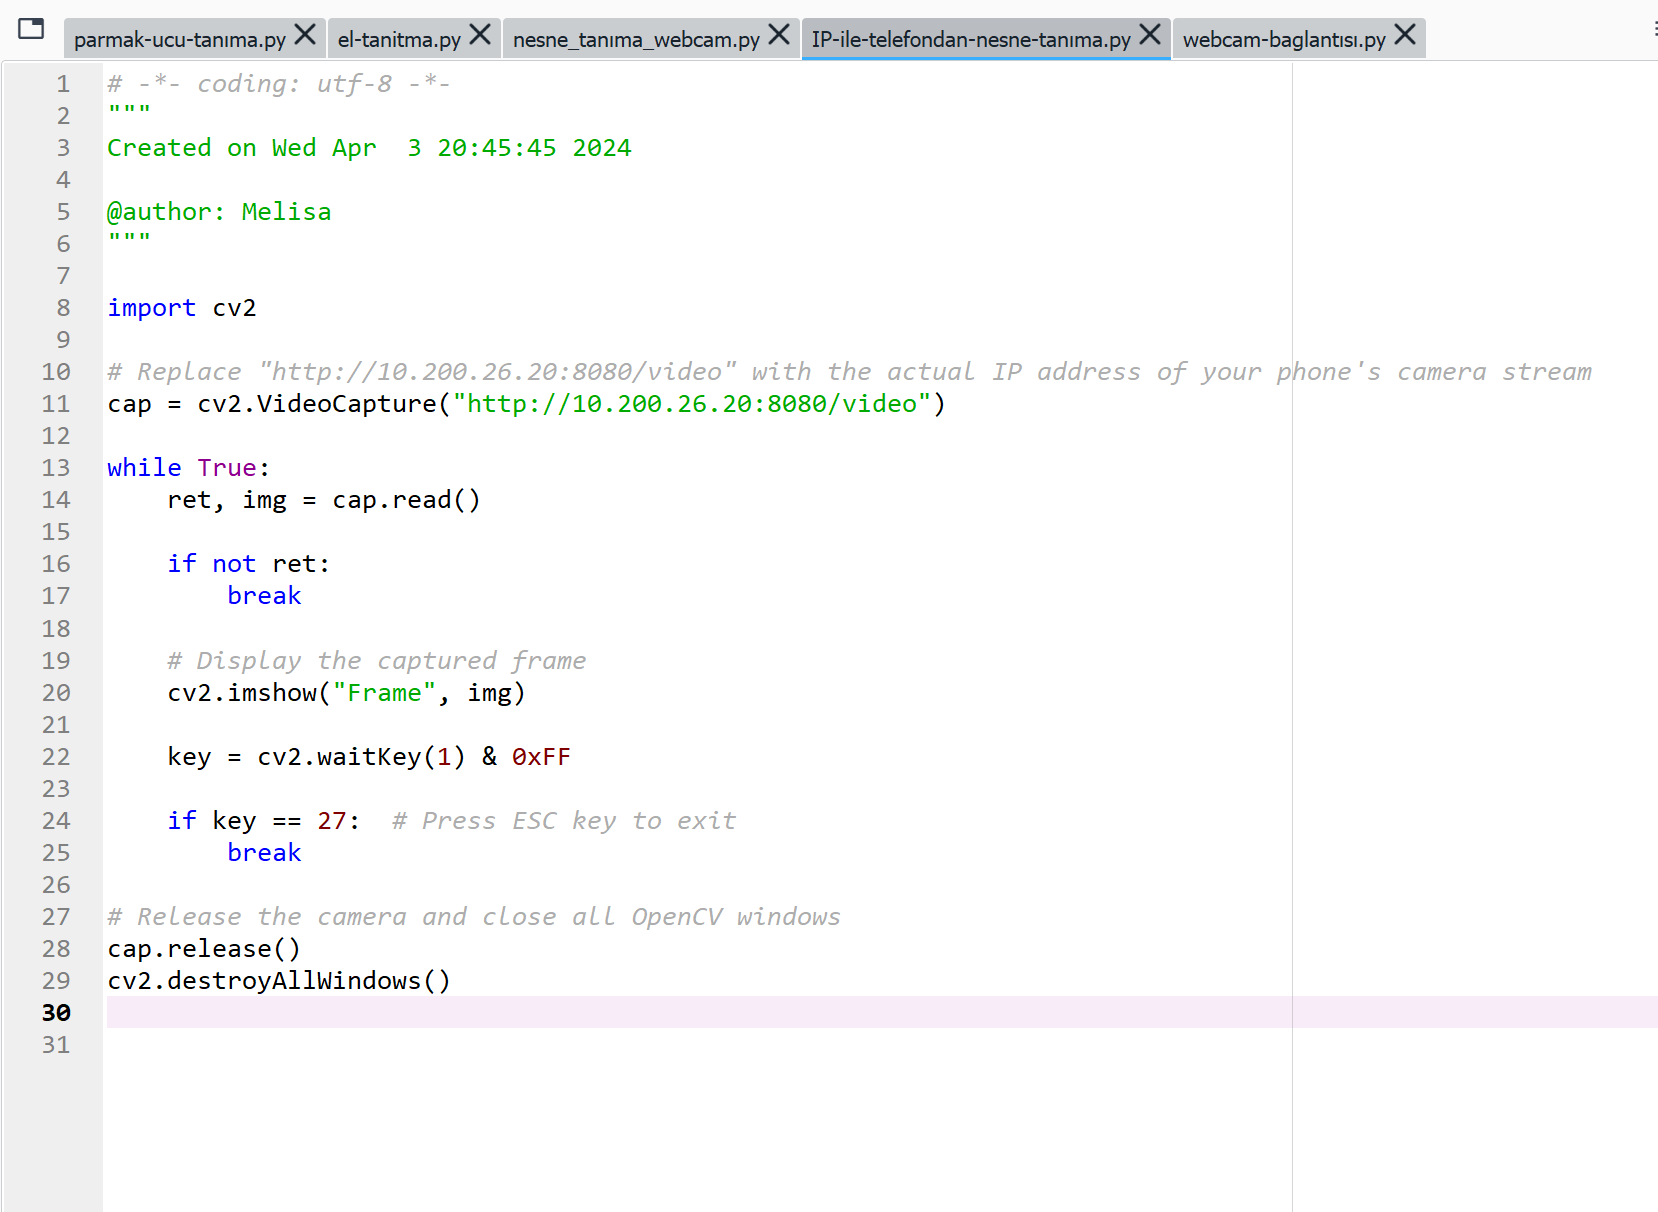
\includegraphics[width=\textwidth]{webcam-telefon-baglama3}
		\caption{Webcam telefon Bağlantısı}
		\label{fig:ornek2}
	\end{figure}
	\newpage
	
	Şekil-\ref{fig:ornek2} de webcam ile telefon arasında bağlantı kurmak için python kodu gösterilmiştir.
	
	\subsection{Webcam ile Nesne Tanıma Projesi}
	Bu proje kameradan (webcam veya IP kamera gibi) video akışını alarak YOLO (You Only Look Once) nesne tanıma modeli kullanarak çerçevedeki nesneleri tanımlamayı amaçlamaktadır. YOLO, tek bir ağ yapısında nesne tanıma ve konumlandırma yapabilen etkili bir derin öğrenme algoritmasıdır.
	\newpage
	\begin{figure}[!ht]
		\centering
		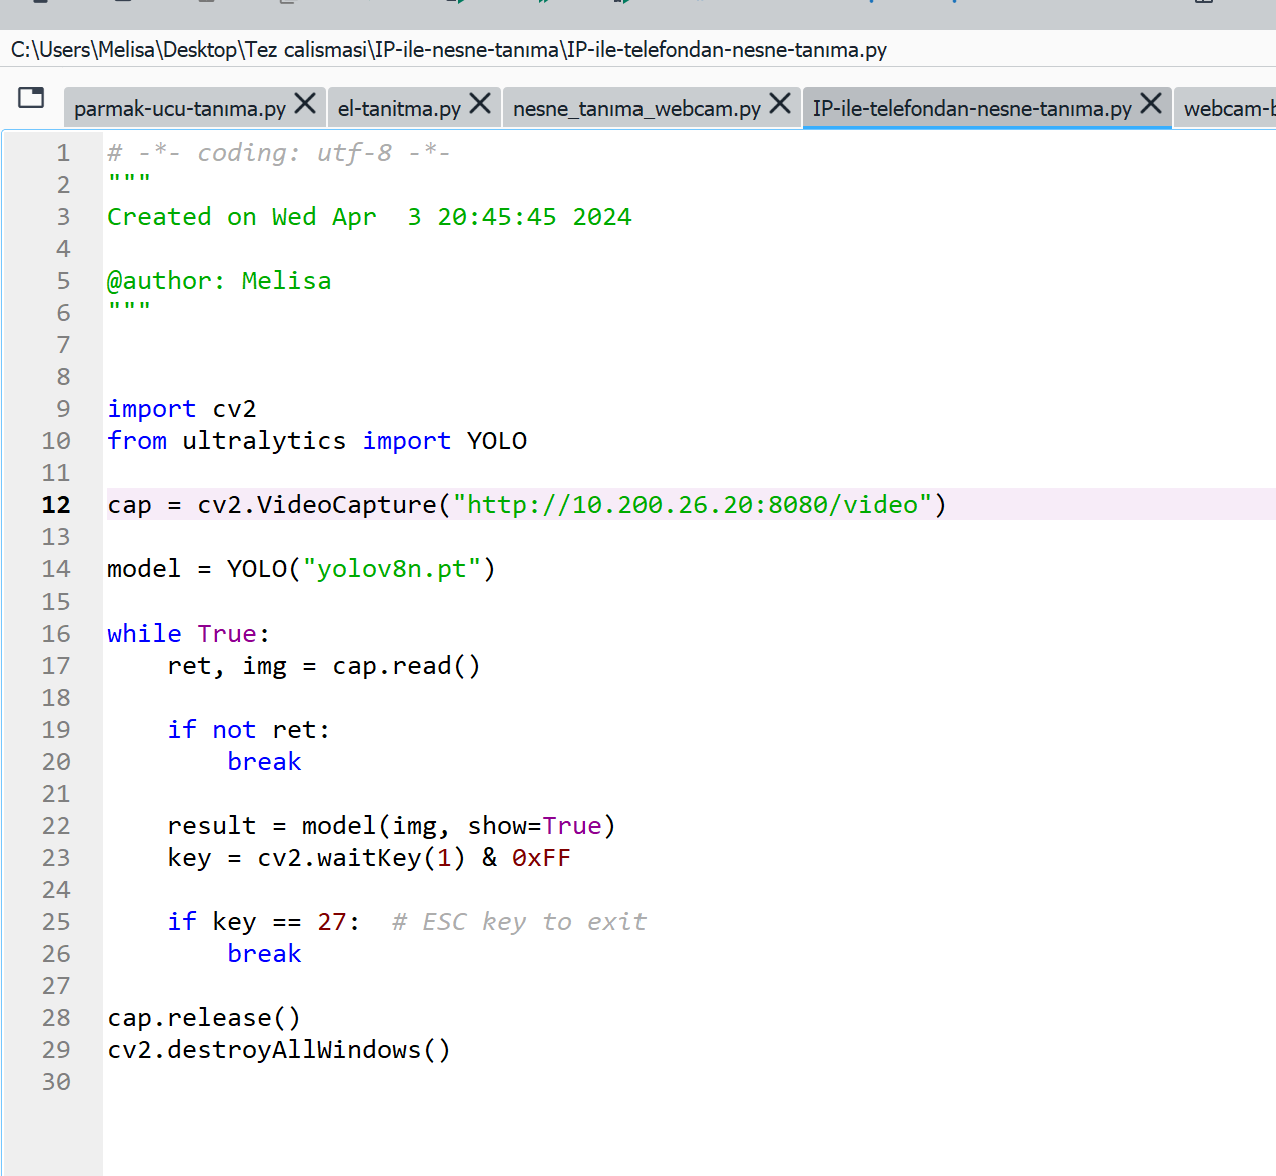
\includegraphics[width=0.7\textwidth]{webcam-telefon-tanima}
		\caption{Webcam Telefon Bağlantısı ve Nesne Tanıma}
		\label{fig:ornek3}
	\end{figure}
	
	Bu projede OpenCV ve YOLO kütüphanesi kullanılmıştır.\newline
	
	cv2.VideoCapture kullanılarak video kaynağı belirlenir. Örnek olarak, bir IP kameradan gelen video akışı veya yerel bir web kamerası kullanılabilir. Kodun bu kısmında IP kamera kullanıldığı varsayılmıştır.
	
	\begin{verbatim}
		model = YOLO("yolov8n.pt")
	\end{verbatim}
	
	Burada, YOLO modeli belirli bir ağırlık dosyası (yolov8n.pt) ile yüklenir. Bu ağırlık dosyası, önceden eğitilmiş ve nesne tanıma için kullanılabilir bir model içerir.
	
	\begin{verbatim}
		while True:
		ret, frame = cap.read()
		result = model(frame, show=True)
	\end{verbatim}
	
	Sonsuz bir döngüde, her çerçeve (frame) için \texttt{cap.read()} kullanılarak bir sonraki çerçeve alınır. Daha sonra, alınan çerçeve YOLO modeline (\texttt{model}) iletilir ve \textbf{result} değişkenine nesne tanıma sonuçları atanır. \texttt{show=True} parametresi ile nesne tanıma sonuçları çerçeveye işlenir ve ekranda gösterilir.
	\newline
	
	\textbf{cv2.waitKey(1)} ile bir tuş girişi beklenir. Eğer kullanıcı "ESC" tuşuna (27 değeri) basarsa, döngüden çıkılır ve program sonlanır.\cite{Nesne-Tanımlama}
	
	\clearpage
	
	\section{Proje Çıktısı}
	
	\begin{figure}[!h]
	\centering
	\begin{minipage}{0.45\textwidth} % Sol fotoğraf için minipage
		\centering
		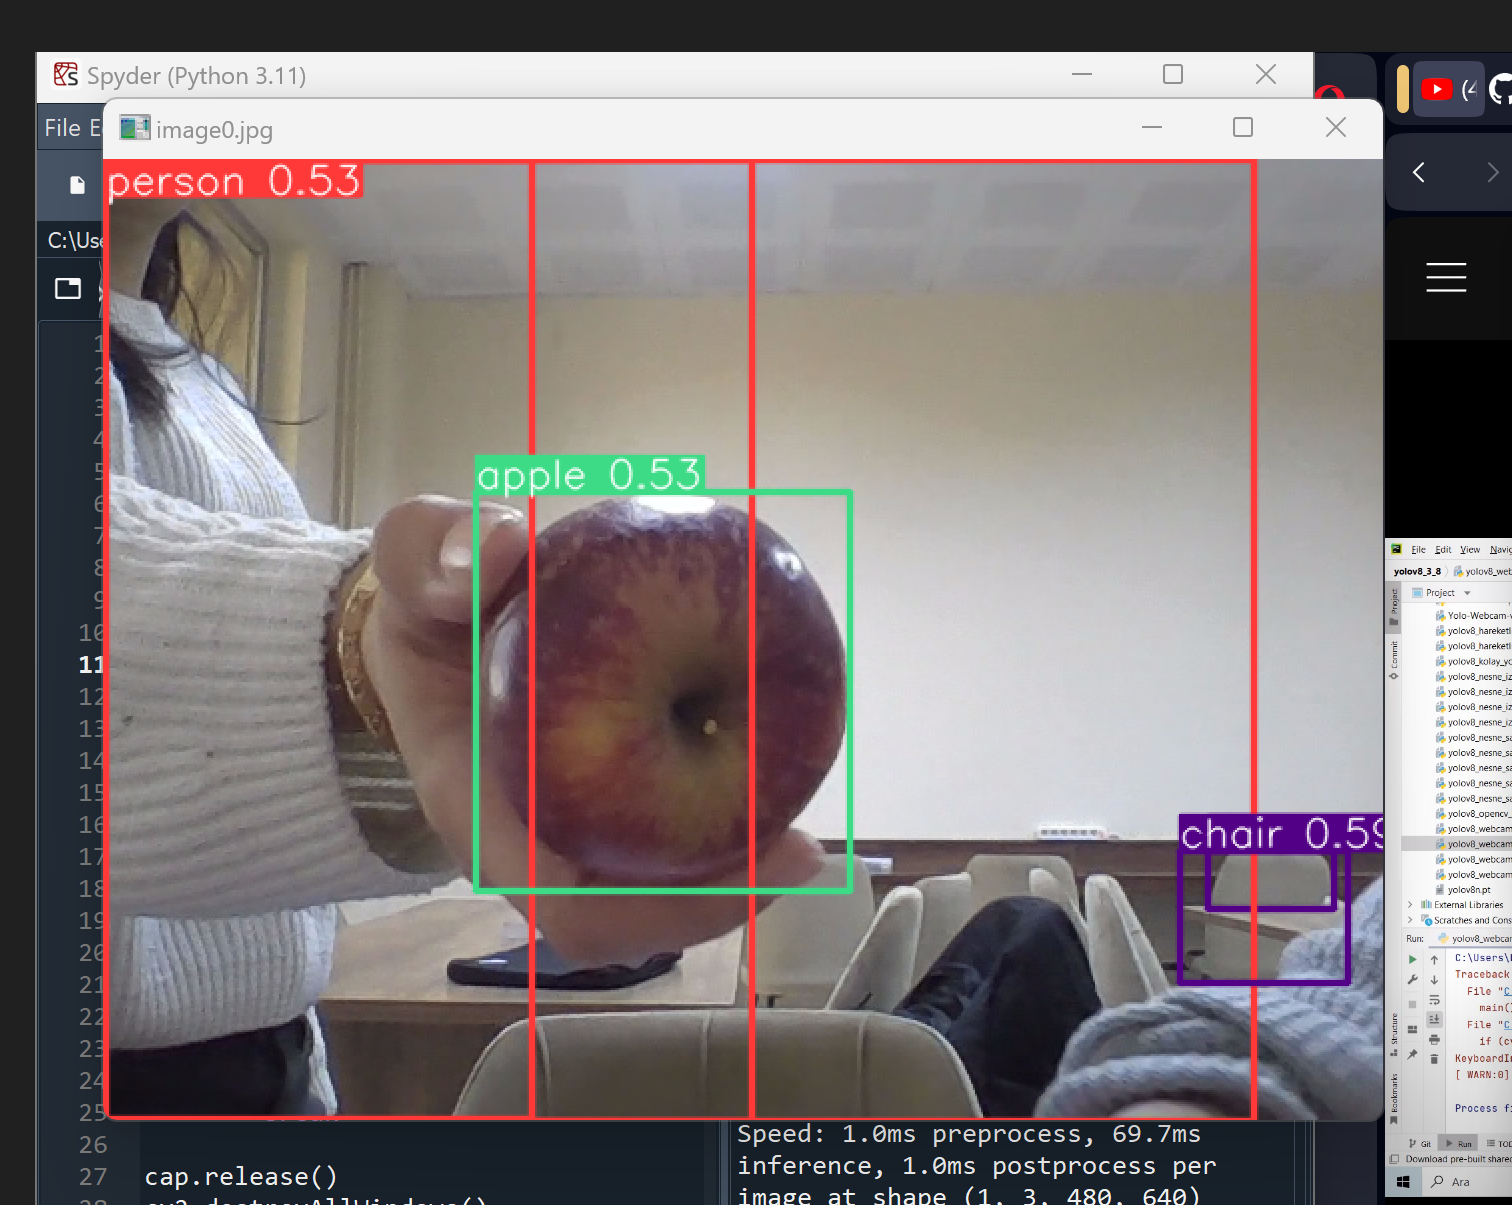
\includegraphics[width=\linewidth]{nesne tanıma-1}
		\label{boyutbulma1}
		\caption*{Şekil-12 (a)}
	\end{minipage}%
	\hfill % Yatay boşluk
	\begin{minipage}{0.45\textwidth} % Sağ fotoğraf için minipage
		\centering
		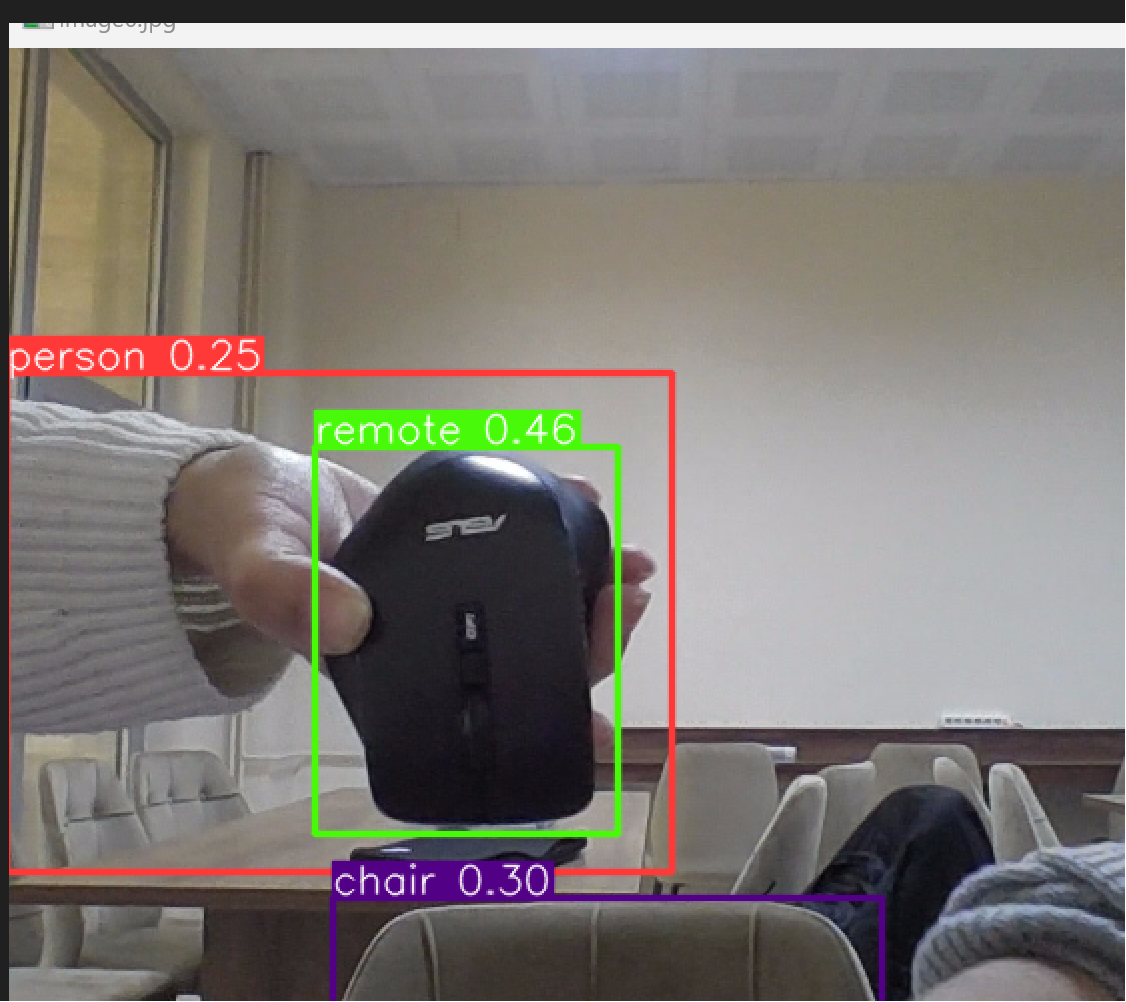
\includegraphics[width=\linewidth]{nesne tanıma-2}
		\label{boyutbulma2}
		\caption*{Şekil-12 (b)}
	\end{minipage}
	
	\vspace{1cm} % Dikey boşluk
	
	\begin{minipage}{\textwidth} % Alt fotoğraf için minipage
		\centering
		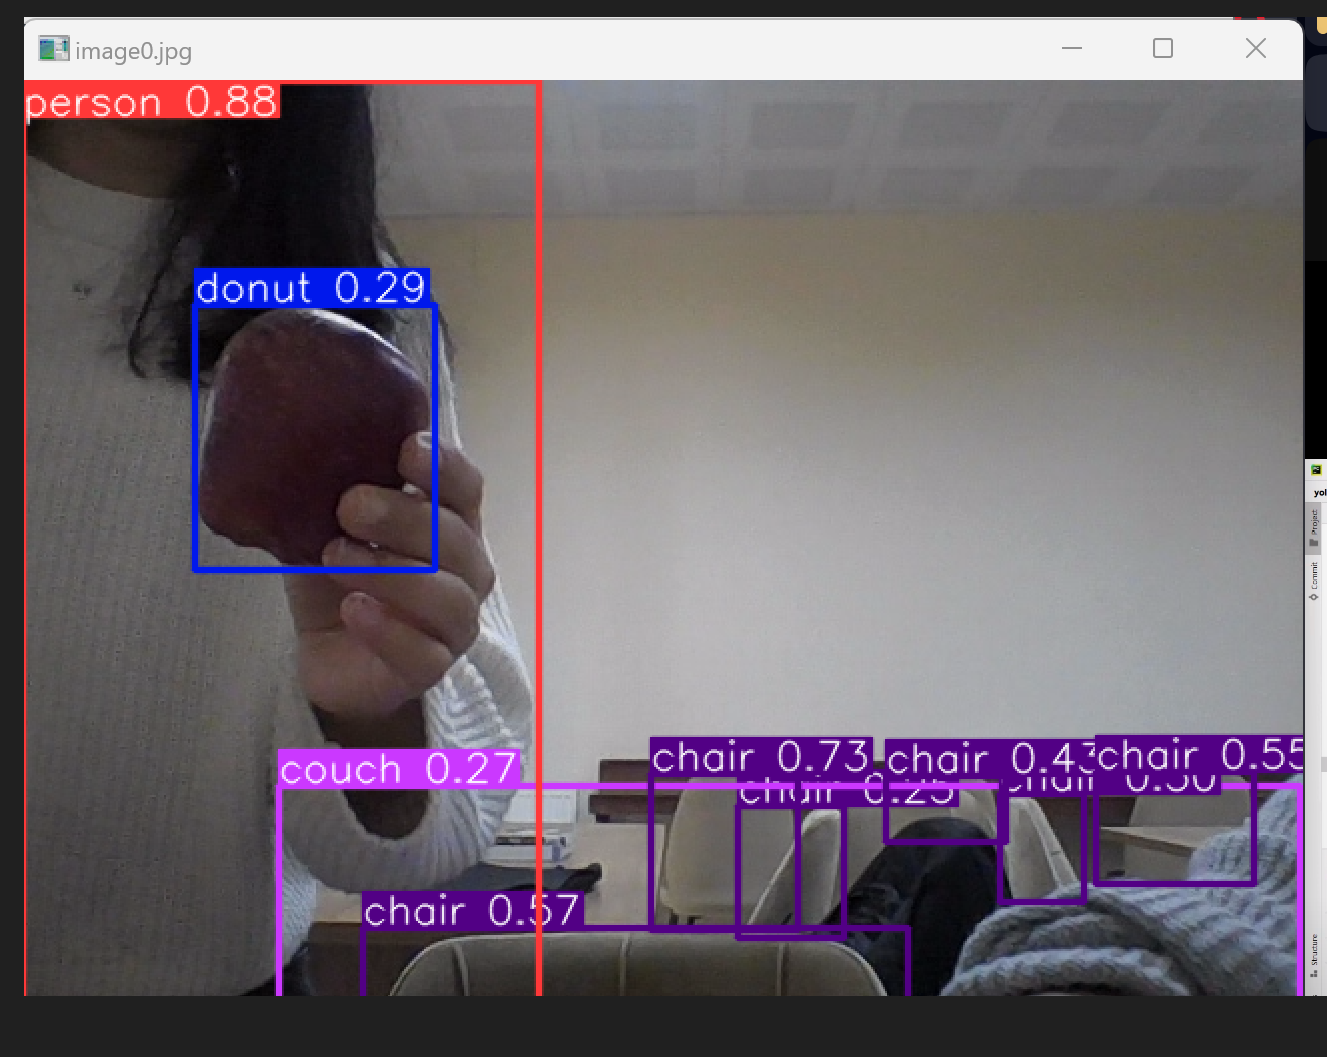
\includegraphics[width=0.5\linewidth]{nesne tanıma-3}
		\caption*{Şekil-12 (c)}
		\label{boyutbulma3}
	\end{minipage}
	
	\caption{Hatalı Nesne Ölçümü} % Üç fotoğrafın altına tek açıklama
	\label{el-nesne-boyutlar}
\end{figure}
	
	\newpage
	\subsection{Nesnelerin güven skorunun belirlenmesi:}
	\textbf{Güven skoru:} Bu skor modelin geçerli ızgara içinde nesne bulunup bulunmadığından ne kadar emin olduğunu gösterir. (0 ise kesinlikle yok 1 ise kesinlikle var) Eğer nesne olduğunu düşünürse de bu nesnenin gerçekten o nesne olup olmadığından ve etrafındaki kutunun koordinatlarından ne kadar emin olduğunu gösterir\cite{picskin2016opencv}.
	\newline
	
	$ \text{Güven Skoru} = \text{Pr(obj)} \times \text{IoU} $
	\newline
	
	Pr(obj): ızgara içinde nesnenin bulunma olasılığı
	
		\subsection{Nesnelerin gerçek boyutları nasıl bulunur?}
	
	Bir görüntüdeki nesnelerin boyutlarını belirleme işlemi genellikle kameradan elde edilen piksel cinsinden bilgileri gerçek dünya koordinatlarına dönüştürmekle başlar. Bu dönüşümü yapabilmek için kameranın kalibrasyon parametrelerine ve bir referans nesnenin gerçek dünya boyutlarına ihtiyaç vardır.
	
	
	\begin{equation}
		\begin{bmatrix}
			X \\
			Y \\
			Z
		\end{bmatrix} = \begin{bmatrix}
			R_{11} & R_{12} & R_{13} \\
			R_{21} & R_{22} & R_{23} \\
			R_{31} & R_{32} & R_{33}
		\end{bmatrix} \cdot \begin{bmatrix}
			x \\
			y \\
			z
		\end{bmatrix} + \begin{bmatrix}
			T_{x} \\
			T_{y} \\
			T_{z}
		\end{bmatrix}
	\end{equation}
	\begin{itemize}

	\item X,Y,Z: Nesnenin dünya koordinatları
	\item x,y,z: Pikselin kamera koordinatları
	\item R: Döndürme matrisi
	\item T: Döndürme matrisine göre çeviri vektörü
	
	Ancak, bu denklem doğrudan görüntüdeki bir nesnenin boyutunu hesaplamak için yetersizdir. Bunun yerine, bir referans nesnenin piksel ve gerçek dünya boyutları arasındaki ilişki kullanılabilir.
	Varsayalım ki referans nesnenin piksel boyutları 
	(w px,h px) ve gerçek dünya boyutları(w mm,h mm) olarak verilmiştir. Bu durumda piksel boyutları ile gerçek dünya boyutları arasındaki ilişki şu şekildedir:
	
	\end{itemize}
	
	\section{Nesne Boyutunu Bulma Adımları}
	\subsection{Adım 1: Görüntünün Yüklenmesi ve Ölçeklendirilmesi}
	İlk adımda, bir görüntü yüklenir ve isteğe bağlı olarak belirtilen bir ölçekte yeniden boyutlandırılır. Ölçeklendirme, görüntünün işlem süresini azaltmak ve bellek kullanımını kontrol etmek için kullanışlıdır. Örneğin, büyük bir görüntüyü işlerken bilgisayar kaynaklarına daha az yük bindirmek için ölçeklendirme yapılabilir.
	
	\subsection{Adım 2: Önişleme (Preprocessing)}
	Önişleme adımı, görüntü üzerinde bazı ön işlemlerin gerçekleştirildiği aşamadır. Bu adımlar şunları içerir:
	\begin{itemize}
	\item Gri Tonlama (Grayscale): Renkli bir görüntüyü gri tonlamaya dönüştürmek, işlemleri basitleştirmek için yaygın bir adımdır. Gri tonlamalı görüntü, her pikseldeki renk bilgisini tek bir yoğunluk değerinde temsil eder.
	
	\item Gaussian Bulanıklaştırma (Gaussian Blur): Gürültüyü azaltmak ve daha iyi kenar algılaması için görüntüye bir Gaussian filtresi uygulanır. Bu, kenarların daha belirgin olmasını sağlar.
	
	\item Kenar Algılama (Canny Edge Detection): Kenar algılama, görüntüdeki önemli kenarları tespit etmek için kullanılır. Canny kenar algılama, diğer yöntemlere göre daha hassas ve doğru sonuçlar verir.
	
	\item Morfolojik İşlemler (Dilation ve Closing): Dilation, kenarların kalınlığını artırarak görüntüdeki boşlukları doldurur. Closing, kenarları birleştirerek nesnelerin daha düzgün bir şekilde algılanmasını sağlar.
	\end{itemize}
	
	\subsection{Adım 3: Kontur Bulma ve Köşe Noktalarının Tespiti}
	Kontur bulma, görüntüdeki nesnelerin sınırlarını belirlemek için kullanılır. Burada, nesnenin dış sınırlarını çevreleyen bir kontur elde edilir. Bu kontur, nesnenin şeklini ve boyutunu belirlemek için kullanılacaktır.
	
	Kontur tespiti yapıldıktan sonra, nesnenin köşe noktalarını tespit etmek için bir dizi işlem yapılır. Bu köşe noktaları, nesnenin dörtgen bir şekil olduğunu düşünerek, daha sonra perspektif dönüşümü için kullanılacaktır.
	
	\subsection{Adım 4: Perspektif Dönüşümü (Warping)}
	Perspektif dönüşümü adımında, nesnenin görsel olarak düz bir açıdan görülebilmesi için görüntü üzerinde bir dönüşüm yapılır. Bu adım, nesnenin gerçek boyutunu doğru bir şekilde belirleyebilmek için önemlidir. Örneğin, bir A4 kağıdının köşe noktaları belirlenerek bu köşe noktalarından bir dörtgen oluşturulur ve bu dörtgen, görüntüdeki nesnenin yerini temsil eder. Daha sonra bu dörtgen, A4 kağıdının gerçek boyutlarına göre yeniden boyutlandırılır.
	
	\subsection{Adım 5: Boyutların Hesaplanması}
	Perspektif dönüşümü sonrasında, dönüştürülen nesnenin genişliği ve yüksekliği piksel cinsinden hesaplanır. Bu adım, nesnenin görüntü üzerindeki piksel boyutlarını belirler.
	
	\subsection{Adım 6: Piksel Boyutlarının Gerçek Boyutlara Dönüştürülmesi}
	Son olarak, nesnenin piksel boyutları gerçek dünya boyutlarına dönüştürülür. Bu adım, bir referans nesne kullanarak gerçek dünya boyutlarına göre piksel boyutlarının hesaplanmasını içerir. Örneğin, bir A4 kağıdının gerçek boyutlarını biliyorsak ve görüntüdeki A4 kağıdının piksel boyutlarını hesapladıysak, diğer nesnelerin boyutlarını da bu oranlar kullanılarak hesaplayabiliriz.
	
	
	Bu adımlar, nesnenin boyutunu belirlemek için tipik olarak izlenen adımlardır ve bu sürecin bir parçası olarak siyah-beyaz yapma, kenar algılama, kontur bulma ve perspektif dönüşüm gibi işlemler kullanılır. Bu işlemler, nesnenin görüntü üzerindeki belirginliğini artırarak ve perspektif etkisini düzelterek doğru boyutları elde etmeyi sağlar.\cite{Nesne-Boyutunu-Bulma-Adımları}
	\clearpage
	
	\begin{figure}[!h] % Use [p] to place the figure on a separate page
		\centering
		
		\begin{minipage}[t]{0.470\linewidth}
			\centering
			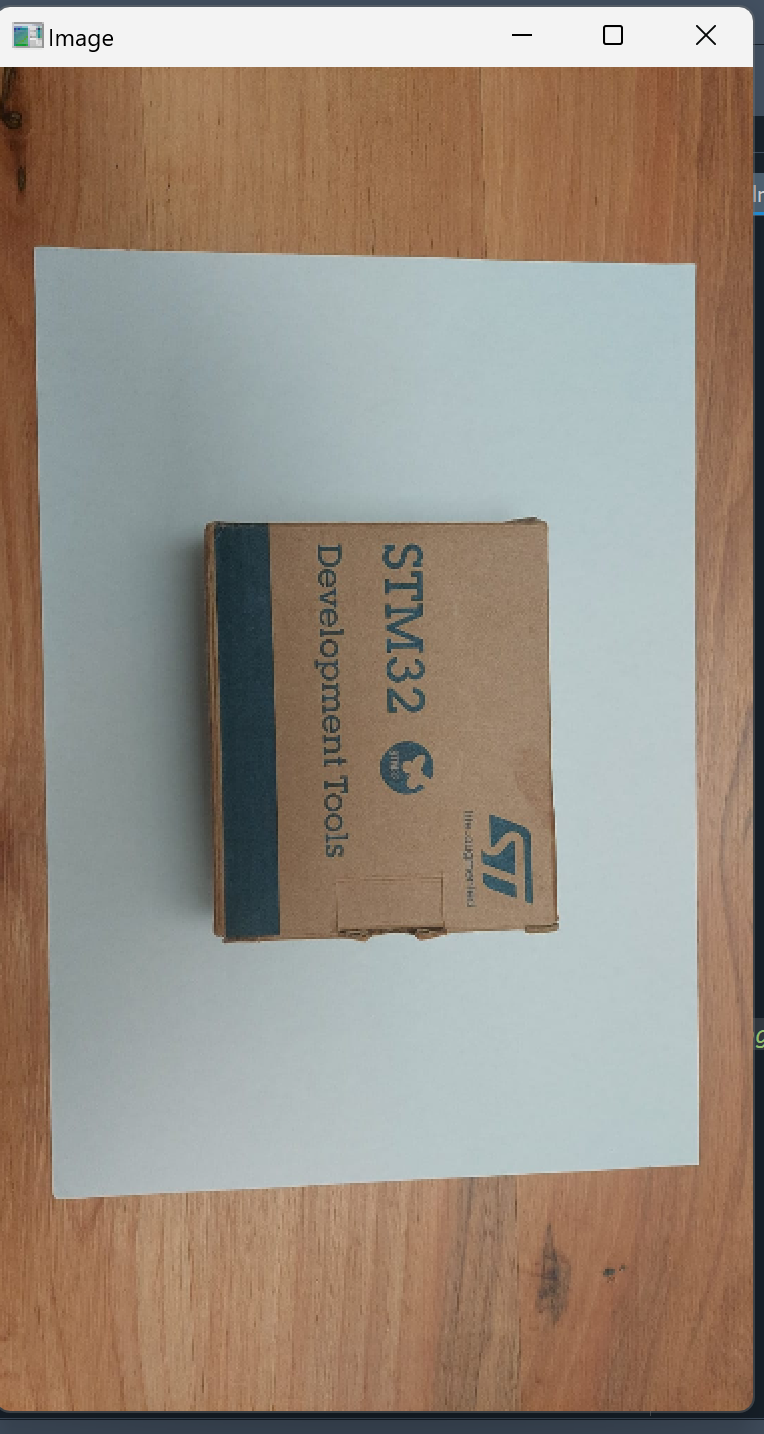
\includegraphics[width=0.65\linewidth]{nesne-1-orijinal}
			\caption*{Şekil-13 (a)}
		\end{minipage}\hfill
		\begin{minipage}[t]{0.470\linewidth}
			\centering
			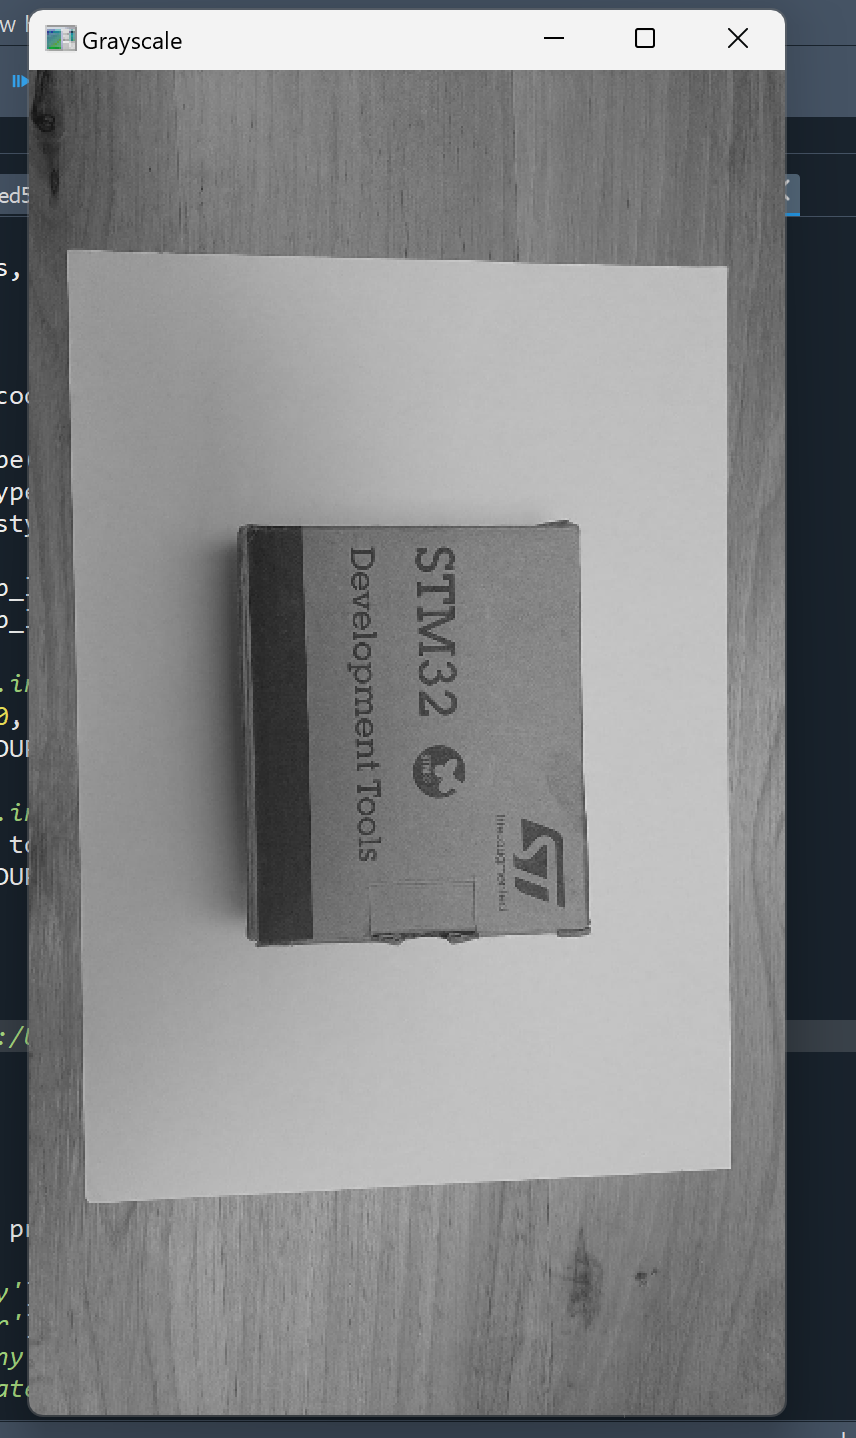
\includegraphics[width=0.65\linewidth]{nesne-1-siyah}
			\caption*{Şekil-13 (b)}
		\end{minipage}
		
			\begin{minipage}[t]{0.470\linewidth}
			\centering
			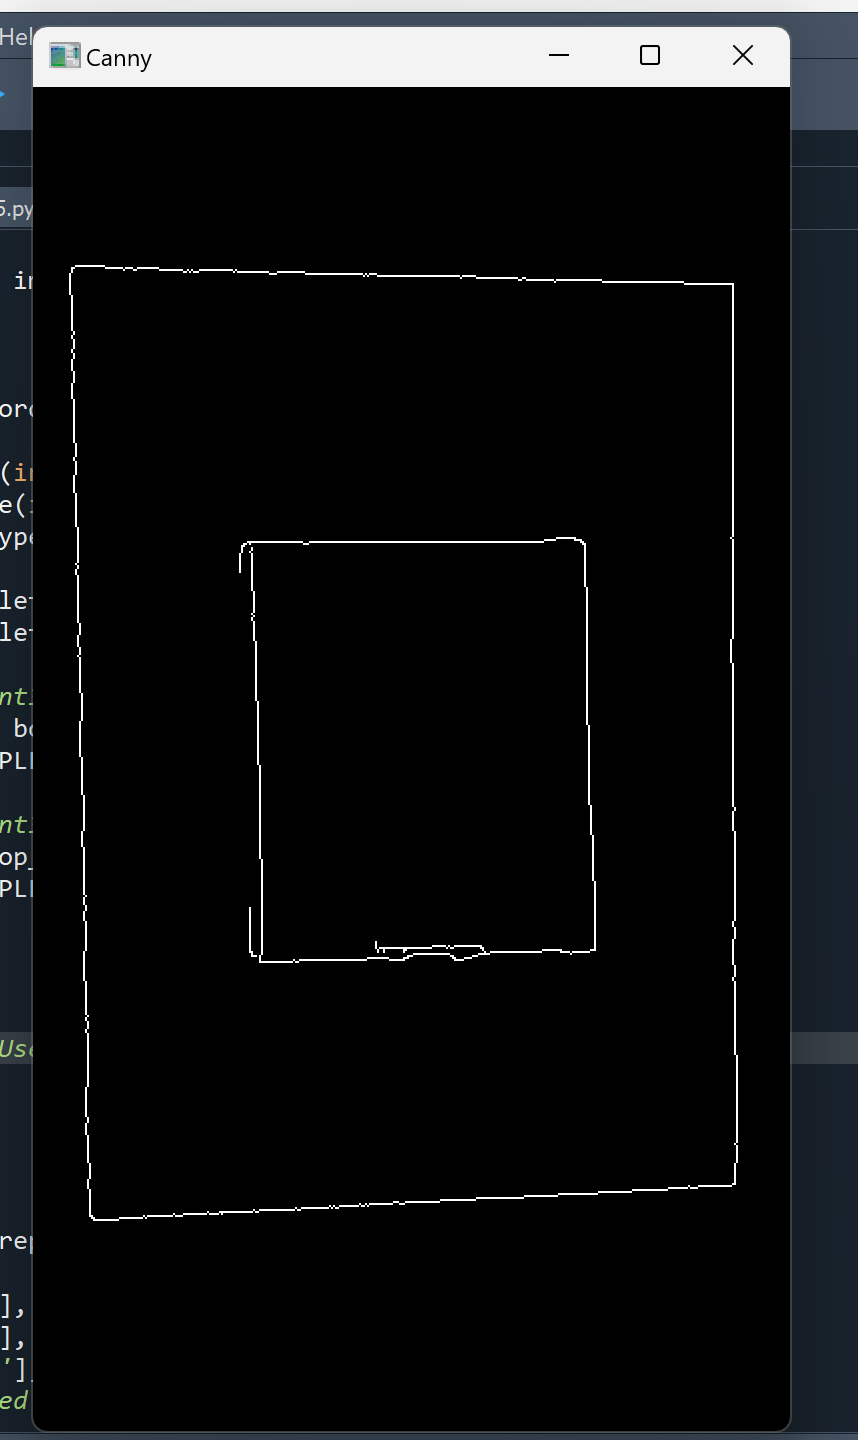
\includegraphics[width=0.65\linewidth]{nesne-1-siyah-beyaz}
			\caption*{Şekil-13 (c)}
		\end{minipage}\hfill
		\begin{minipage}[t]{0.470\linewidth}
			\centering
			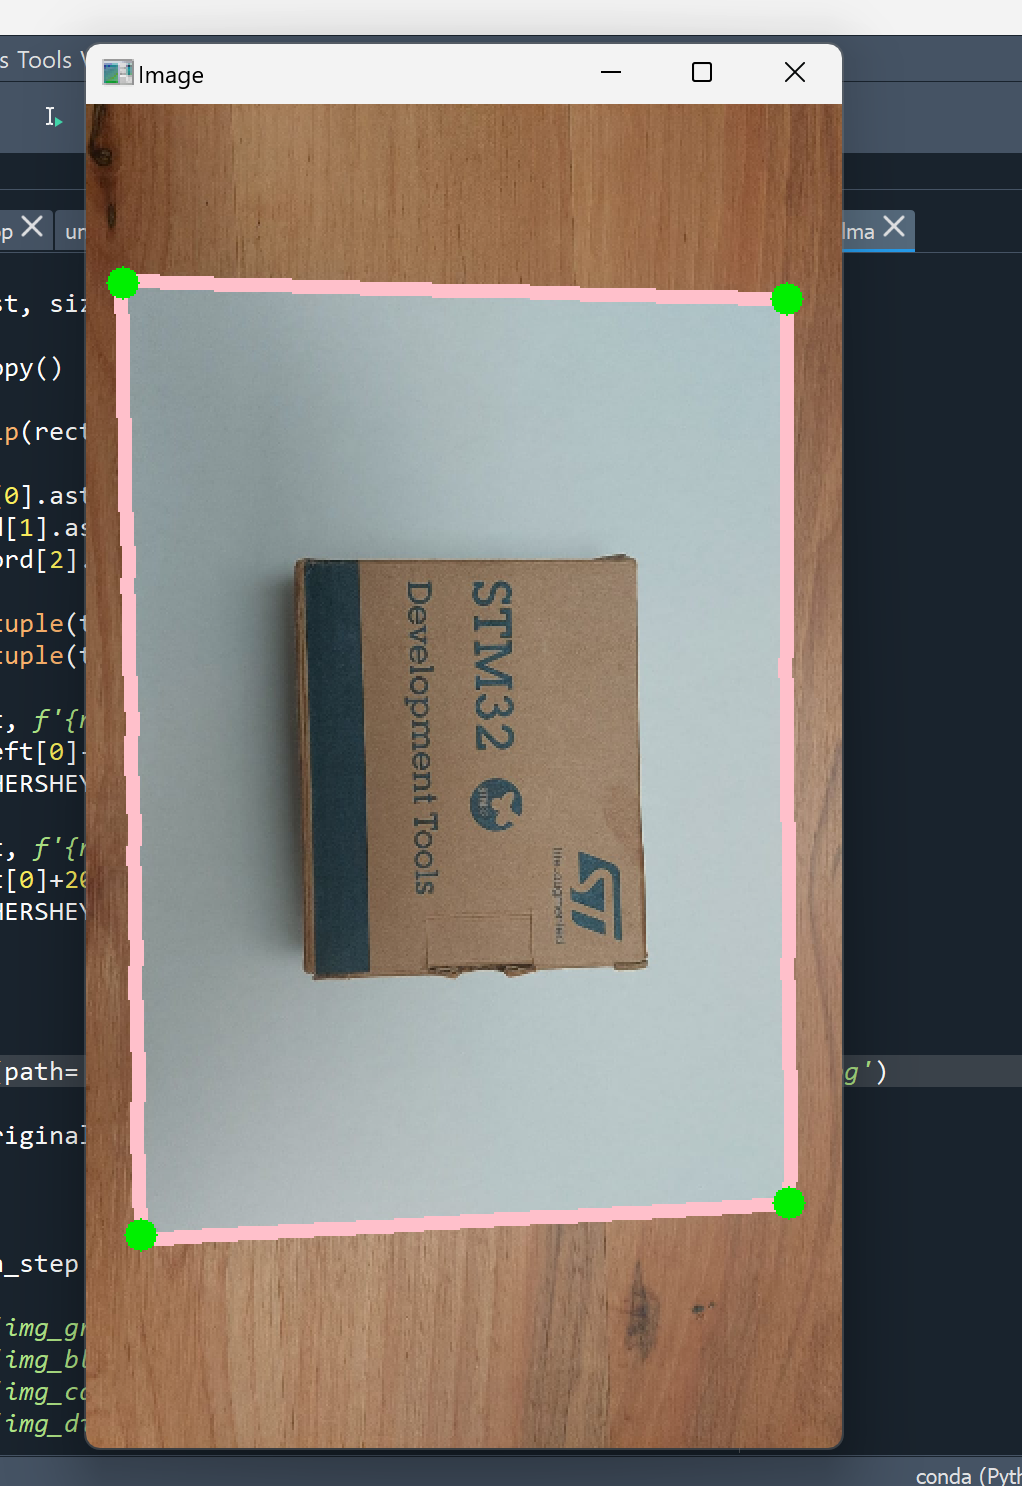
\includegraphics[width=0.65\linewidth]{nesne-1-a4}
			\caption*{Şekil-13 (d)}
		\end{minipage}
			\begin{minipage}[t]{0.470\linewidth}
			\centering
			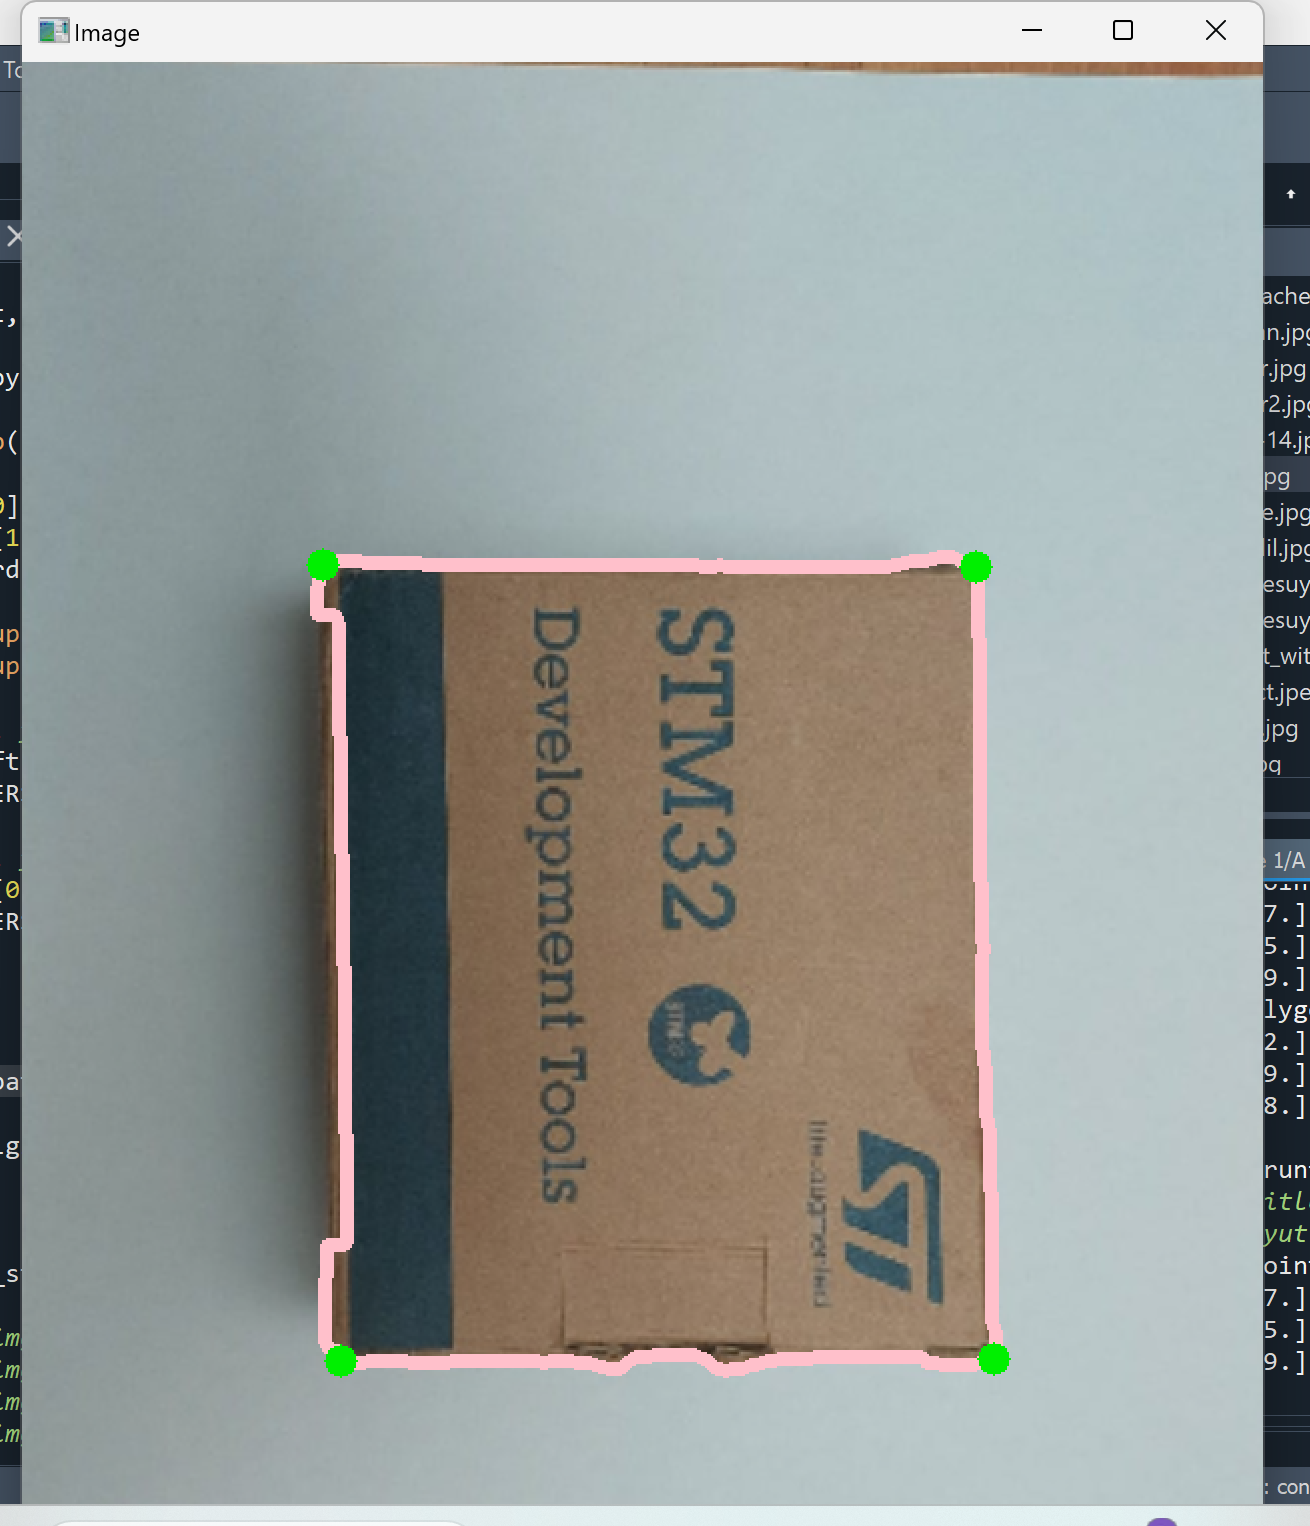
\includegraphics[width=0.65\linewidth]{nesne-1-cerceve}
			\caption*{Şekil-13 (e)}
		\end{minipage}\hfill
		\begin{minipage}[t]{0.470\linewidth}
			\centering
			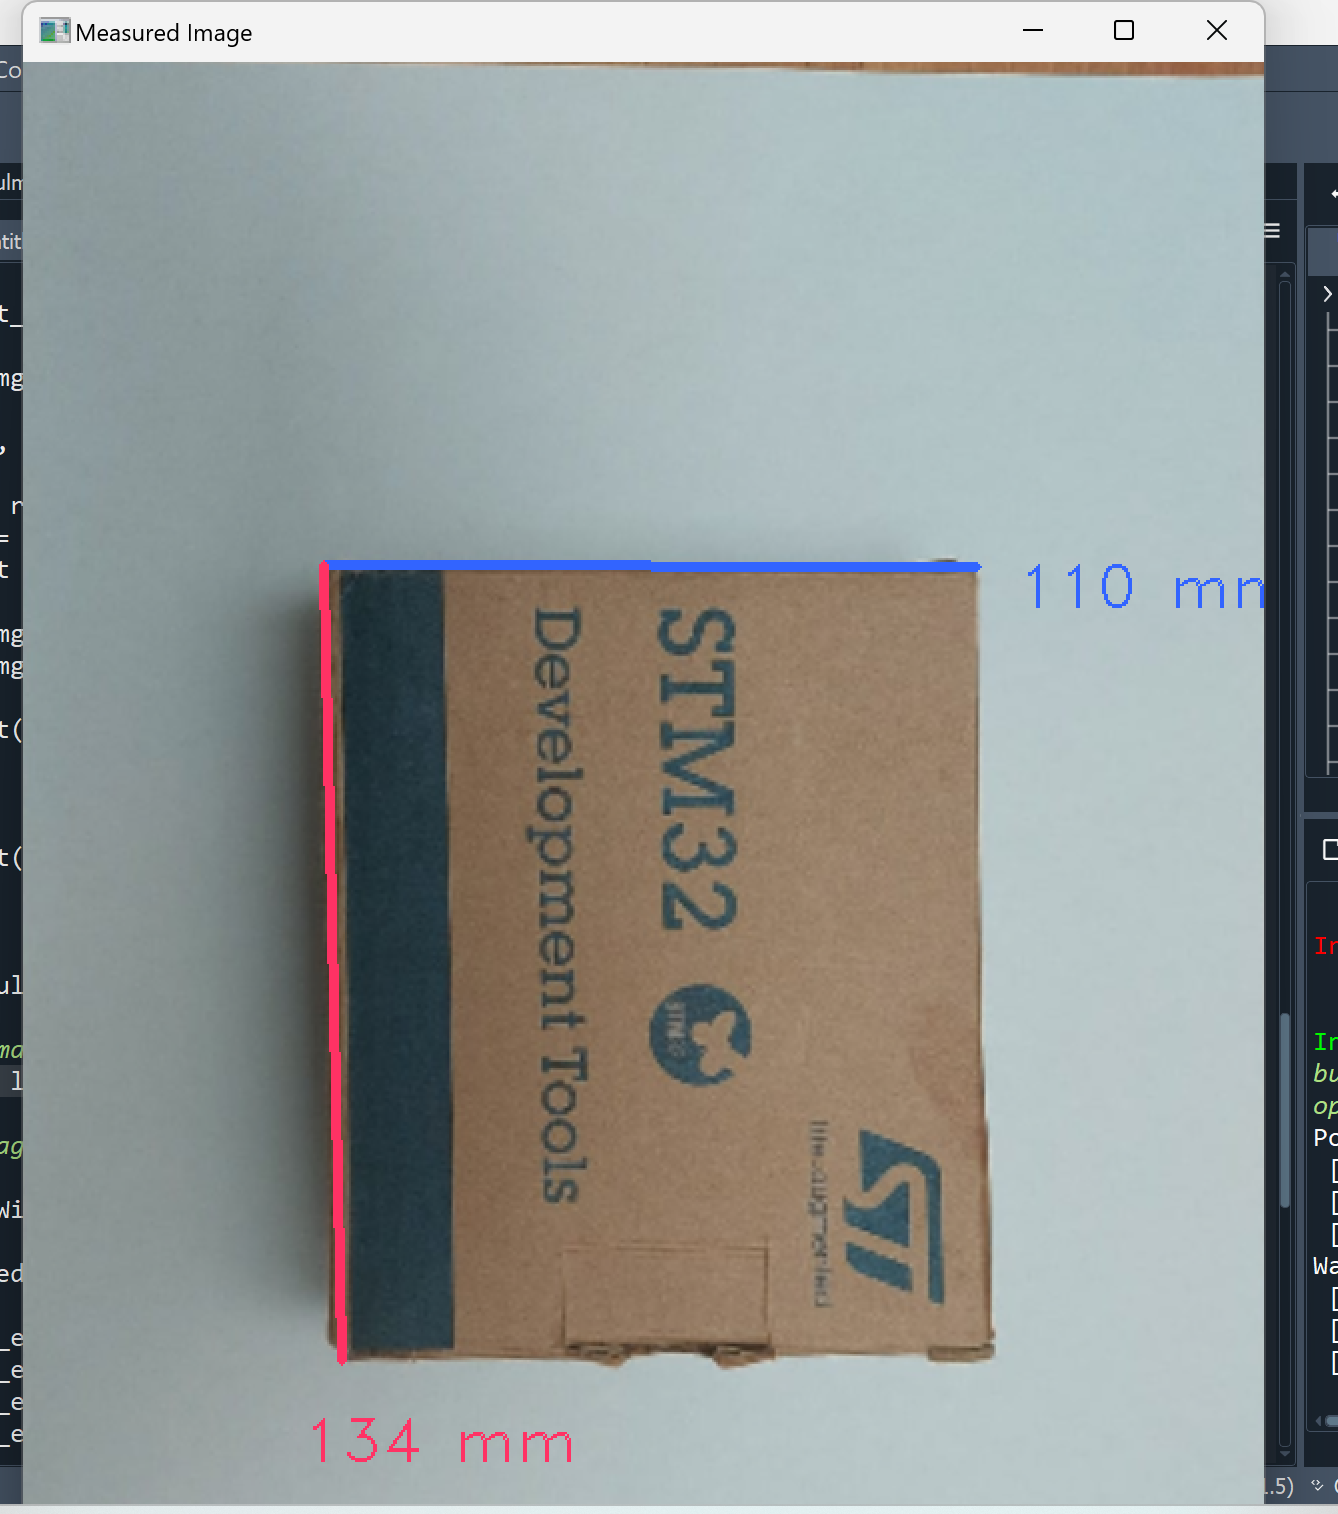
\includegraphics[width=0.65\linewidth]{boyut-bulma-sonuc-1}
			\caption*{Şekil-13 (f)}
		\end{minipage}
			\caption{Kutu boyutu bulma}
	\end{figure}
	\clearpage

	

	
	\begin{figure}[!h] % Use [p] to place the figure on a separate page
		\centering
		
		\begin{minipage}[t]{0.470\linewidth}
			\centering
			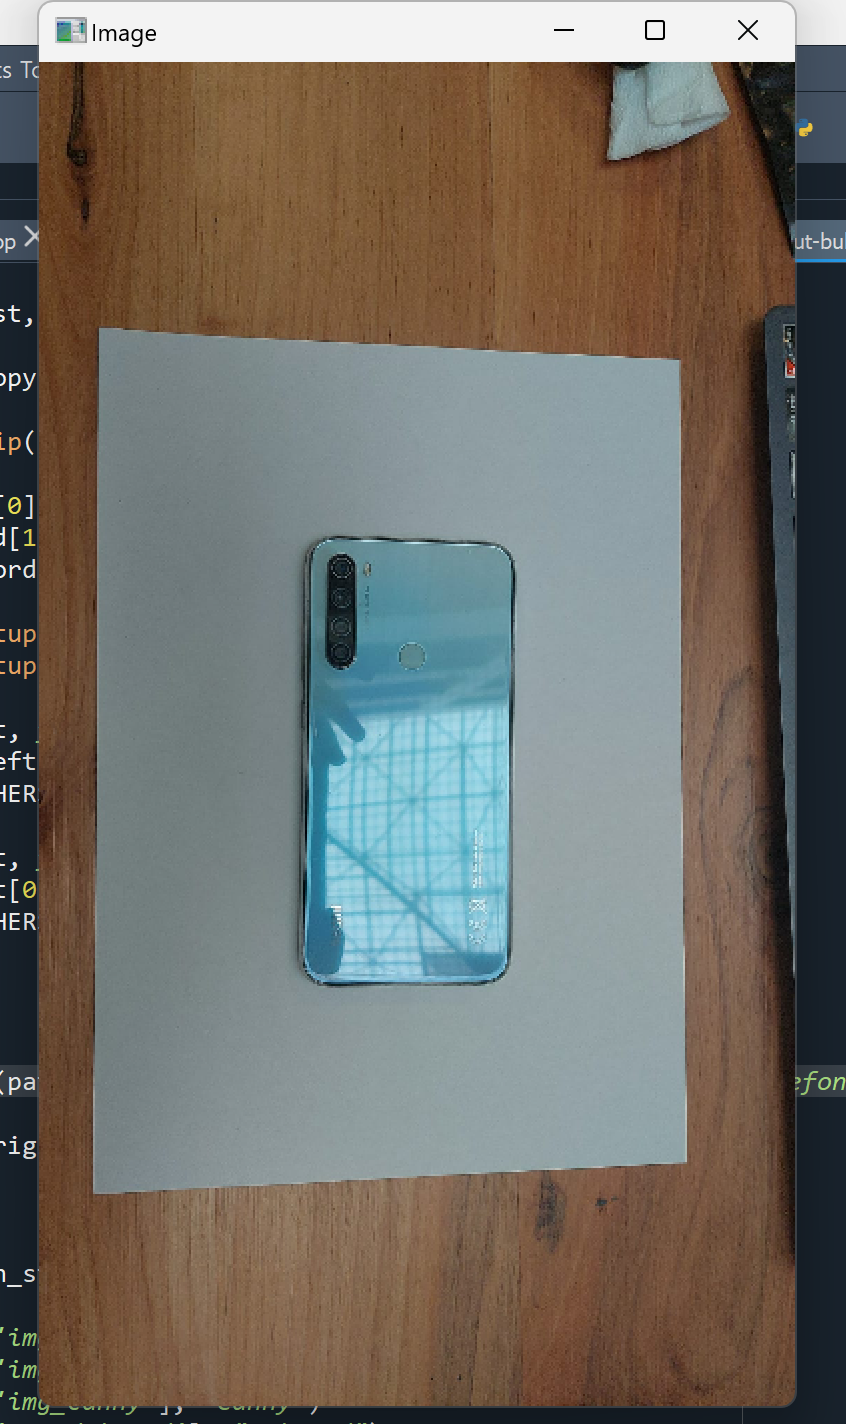
\includegraphics[width=0.65\linewidth]{nesne-3-orijinal}
			\caption*{Şekil-14 (a)}
		\end{minipage}\hfill
		\begin{minipage}[t]{0.470\linewidth}
			\centering
			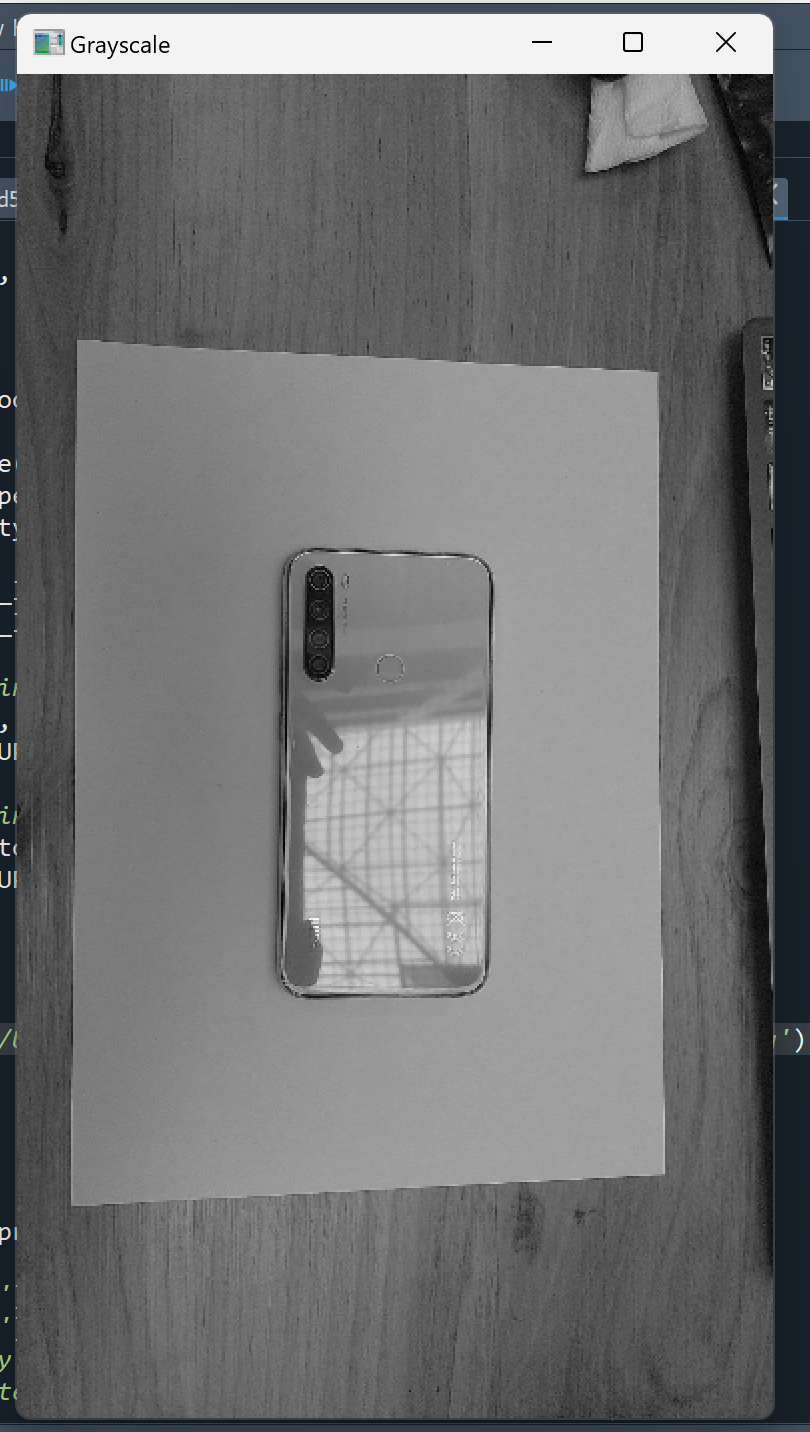
\includegraphics[width=0.65\linewidth]{nesne-3-siyah}
			\caption*{Şekil-14 (b)}
		\end{minipage}
		\begin{minipage}[t]{0.470\linewidth}
			\centering
			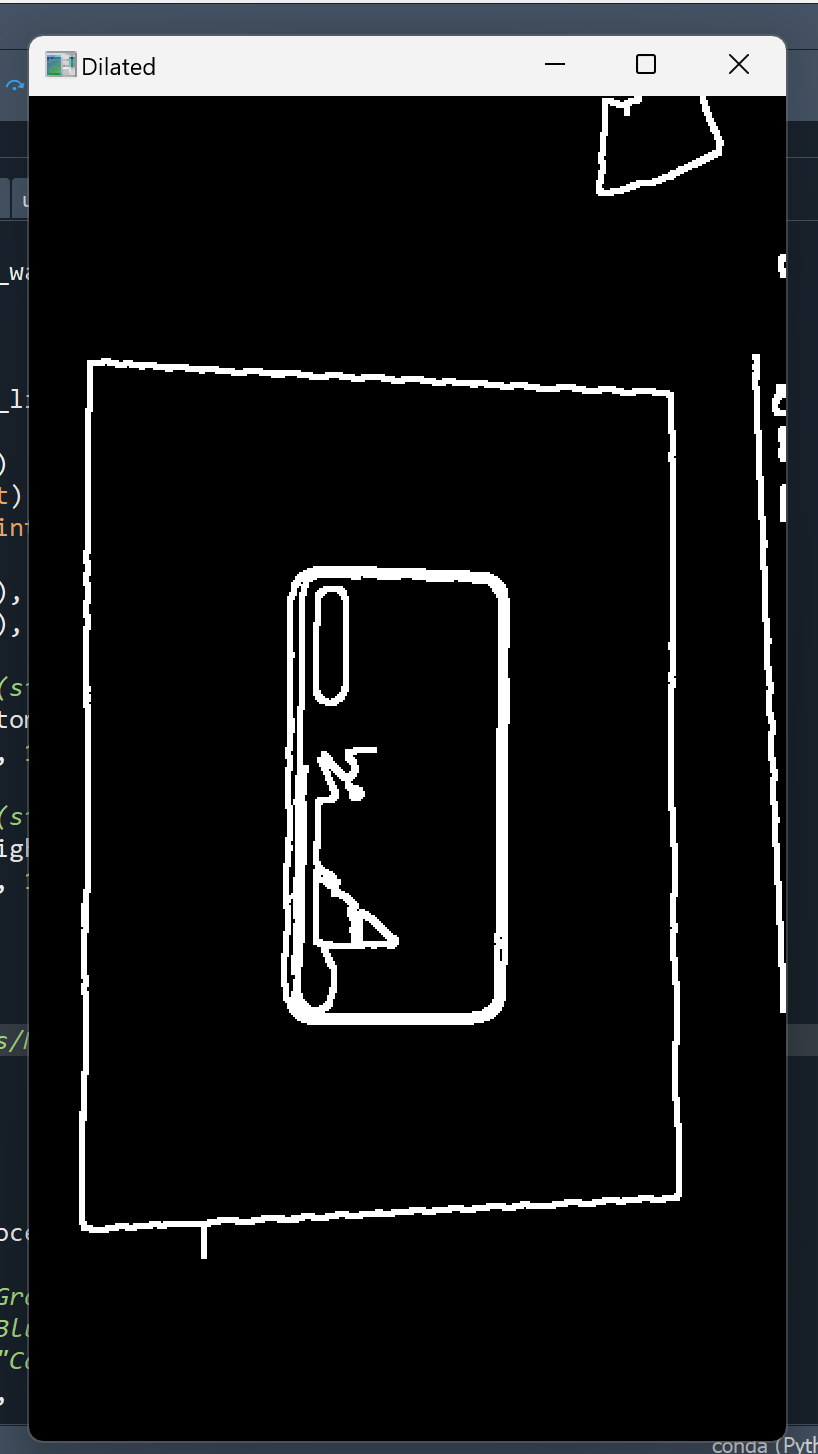
\includegraphics[width=0.65\linewidth]{nesne-3-siyah-beyaz}
			\caption*{Şekil-14 (c)}
		\end{minipage}\hfill
		\begin{minipage}[t]{0.470\linewidth}
			\centering
			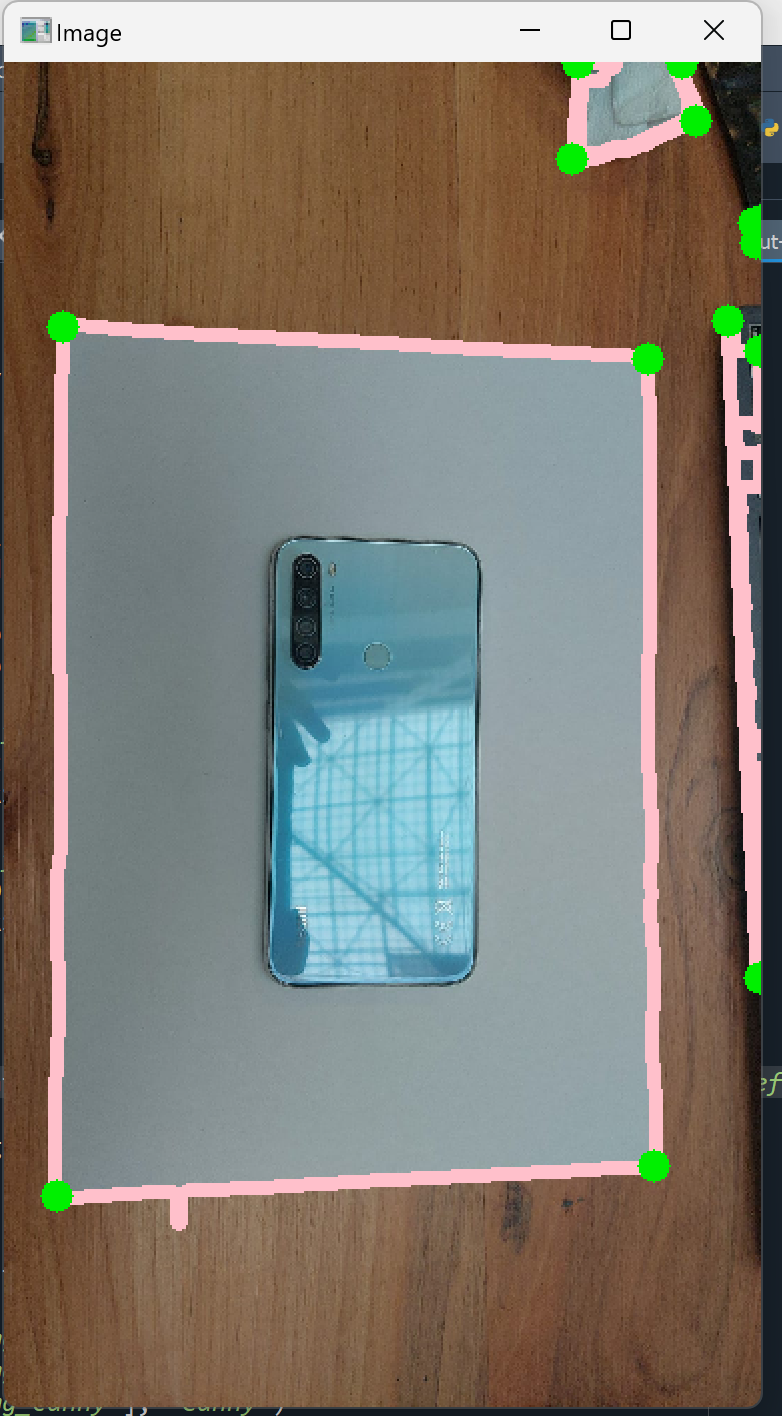
\includegraphics[width=0.65\linewidth]{nesne-3-a4}
			\caption*{Şekil-14 (d)}
		\end{minipage}
			\begin{minipage}[t]{0.470\linewidth}
			\centering
			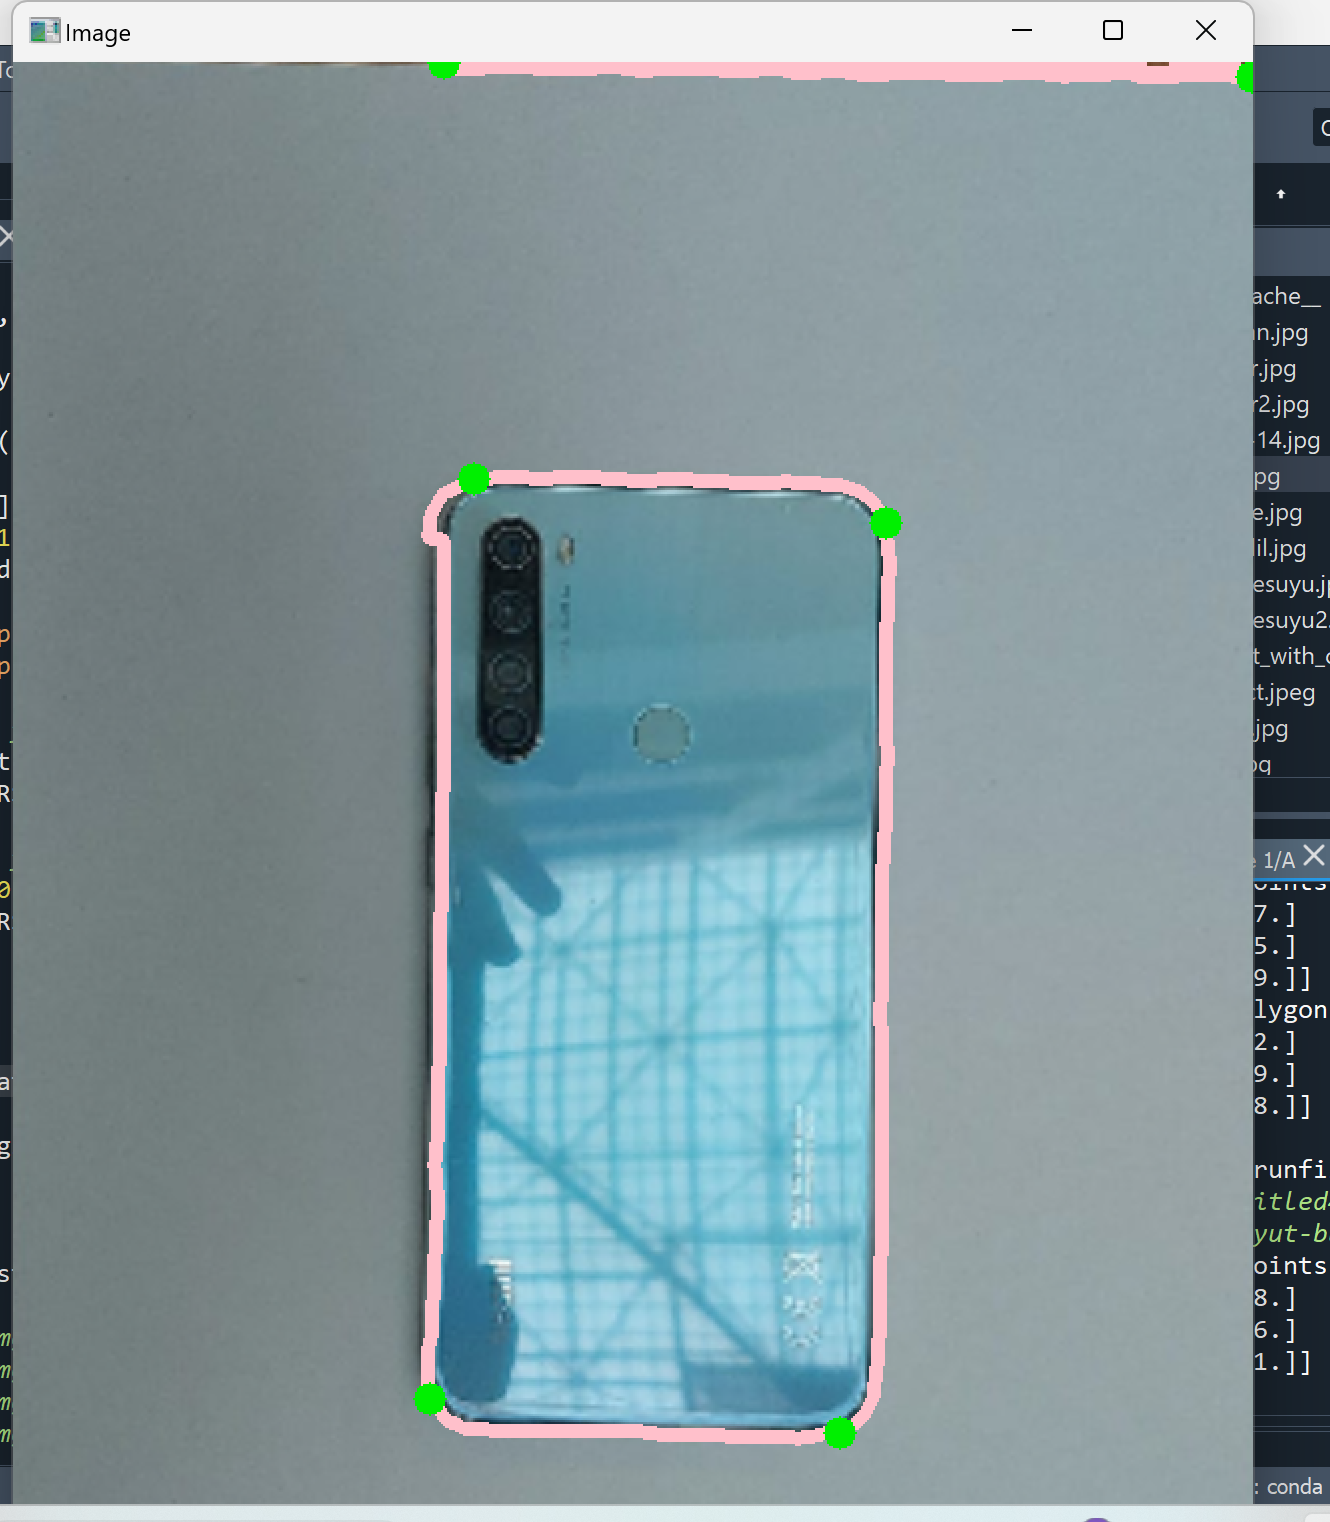
\includegraphics[width=0.65\linewidth]{nesne-3-cerceve}
			\caption*{Şekil-14 (e)}
		\end{minipage}\hfill
		\begin{minipage}[t]{0.470\linewidth}
			\centering
			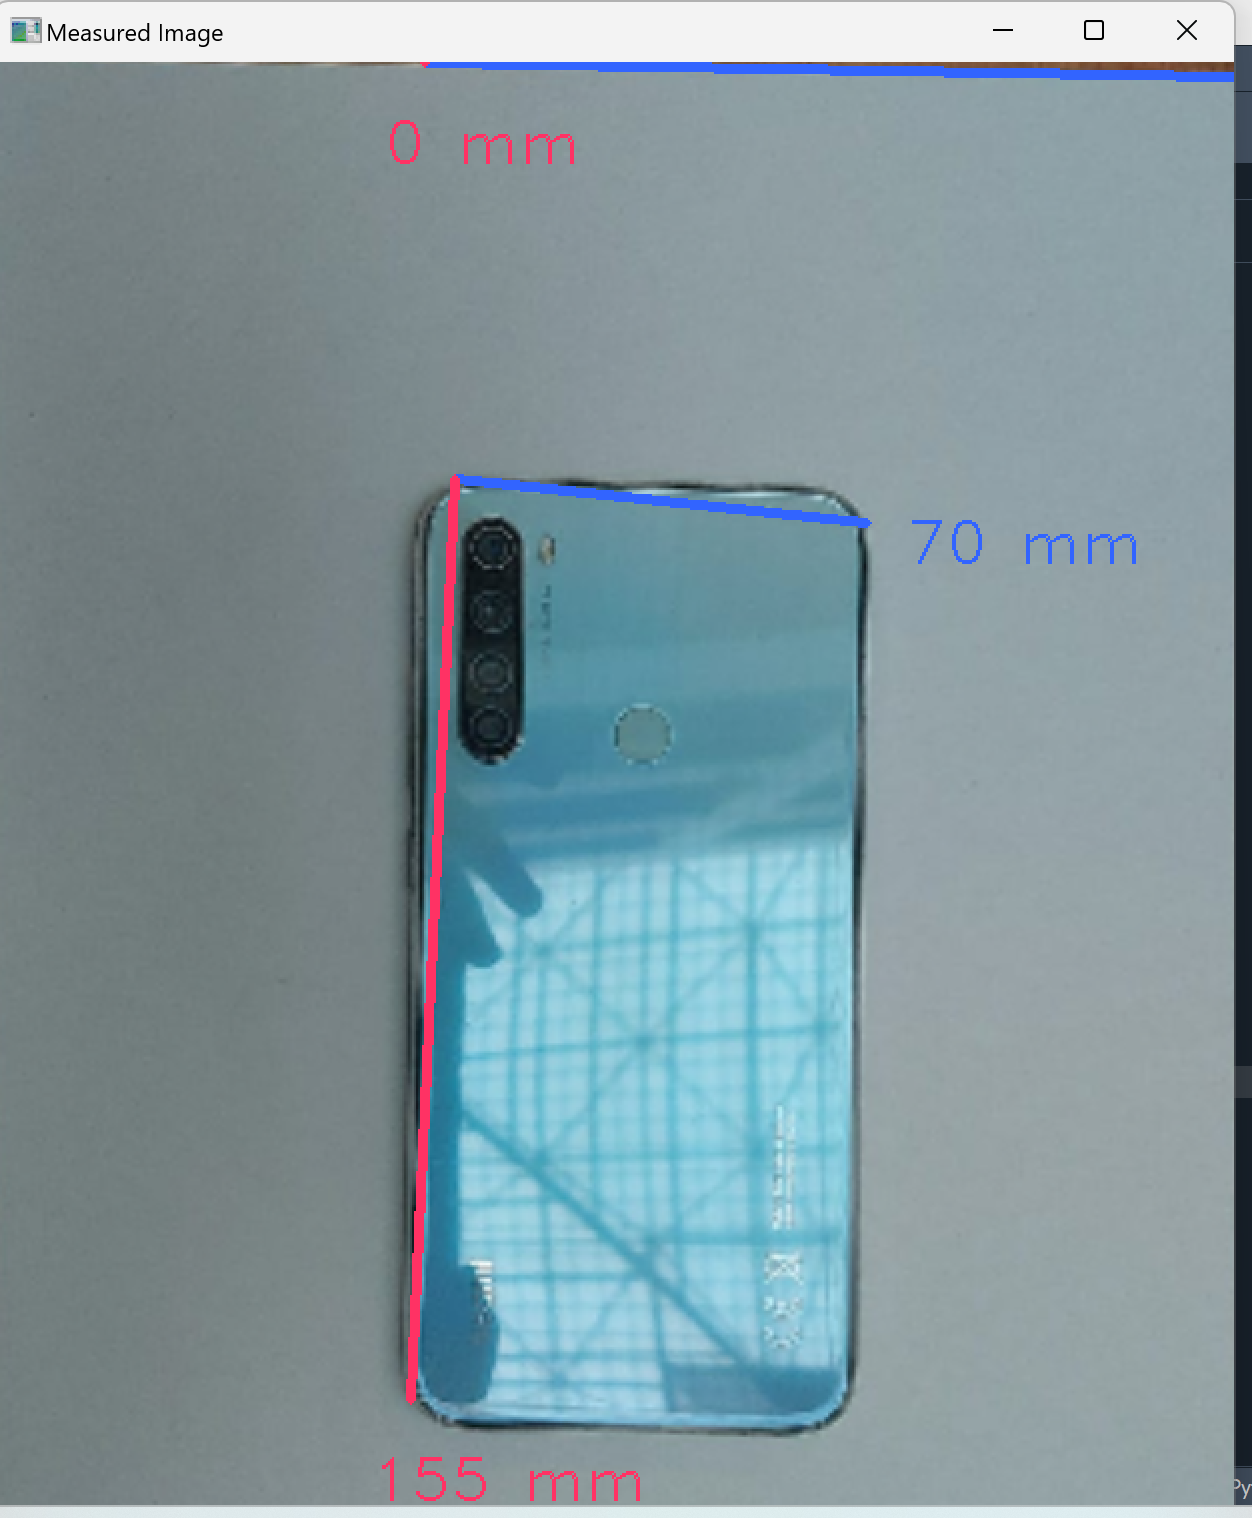
\includegraphics[width=0.65\linewidth]{boyut-bulma-sonuc-3}
			\caption*{Şekil-14 (f)}
		\end{minipage}
		\caption{telefon boyut bulma}
	\end{figure}
	\clearpage

	\begin{figure}[!h] % Use [p] to place the figure on a separate page
		\centering
		
		\begin{minipage}[t]{0.470\linewidth}
			\centering
			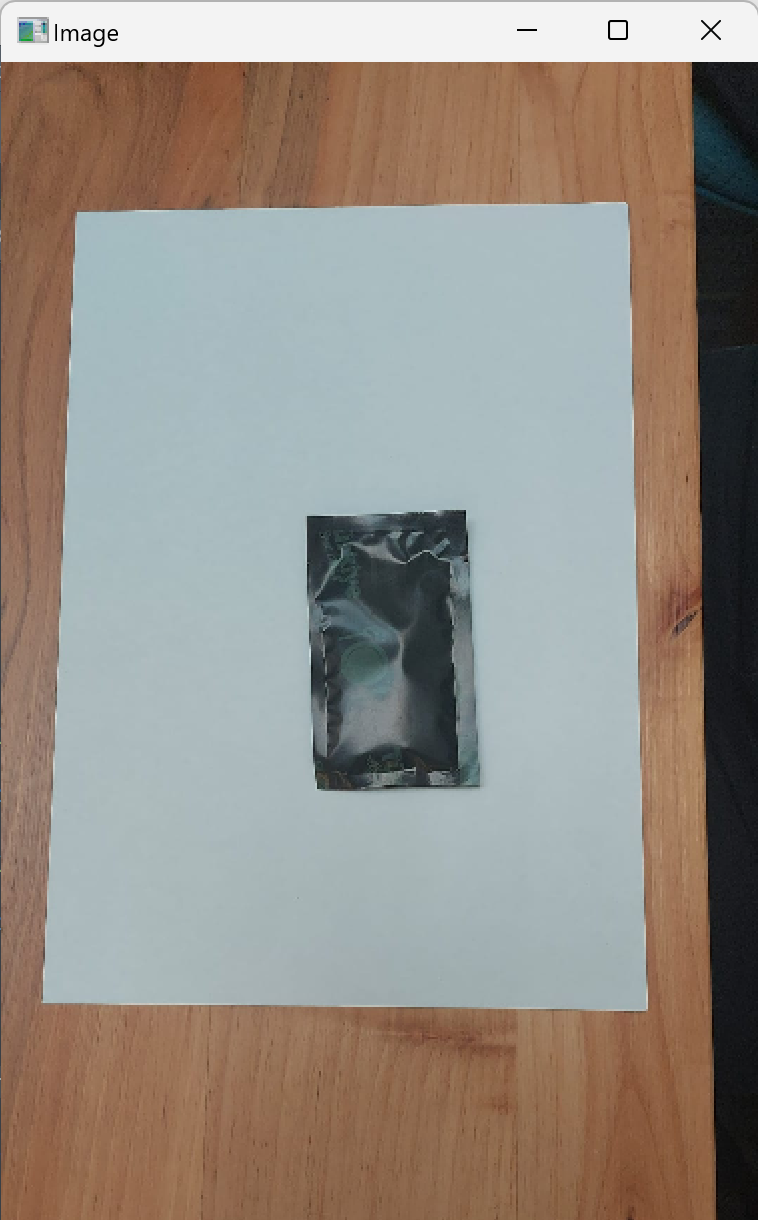
\includegraphics[width=0.65\linewidth]{nesne-2-orijinal}
			\caption*{Şekil-15 (a)}
		\end{minipage}\hfill
		\begin{minipage}[t]{0.470\linewidth}
			\centering
			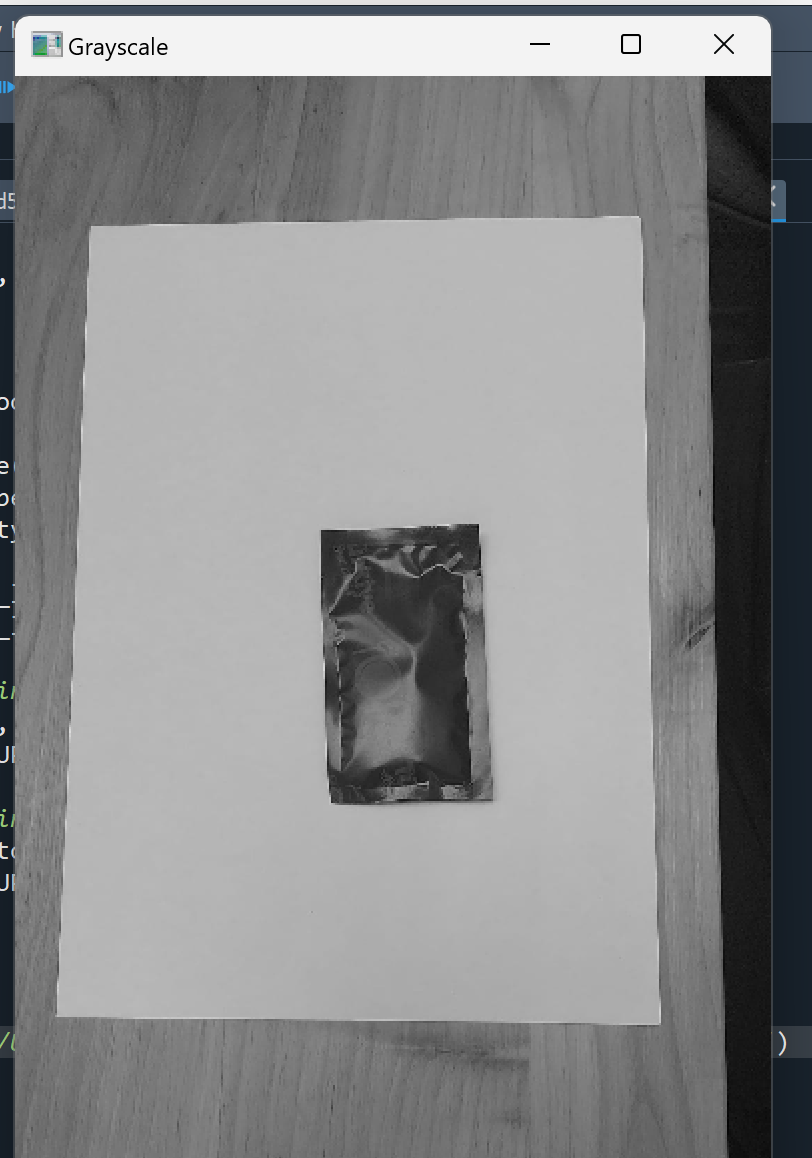
\includegraphics[width=0.65\linewidth]{nesne-2-siyah}
			\caption*{Şekil-15 (b)}
		\end{minipage}
			\begin{minipage}[t]{0.470\linewidth}
			\centering
			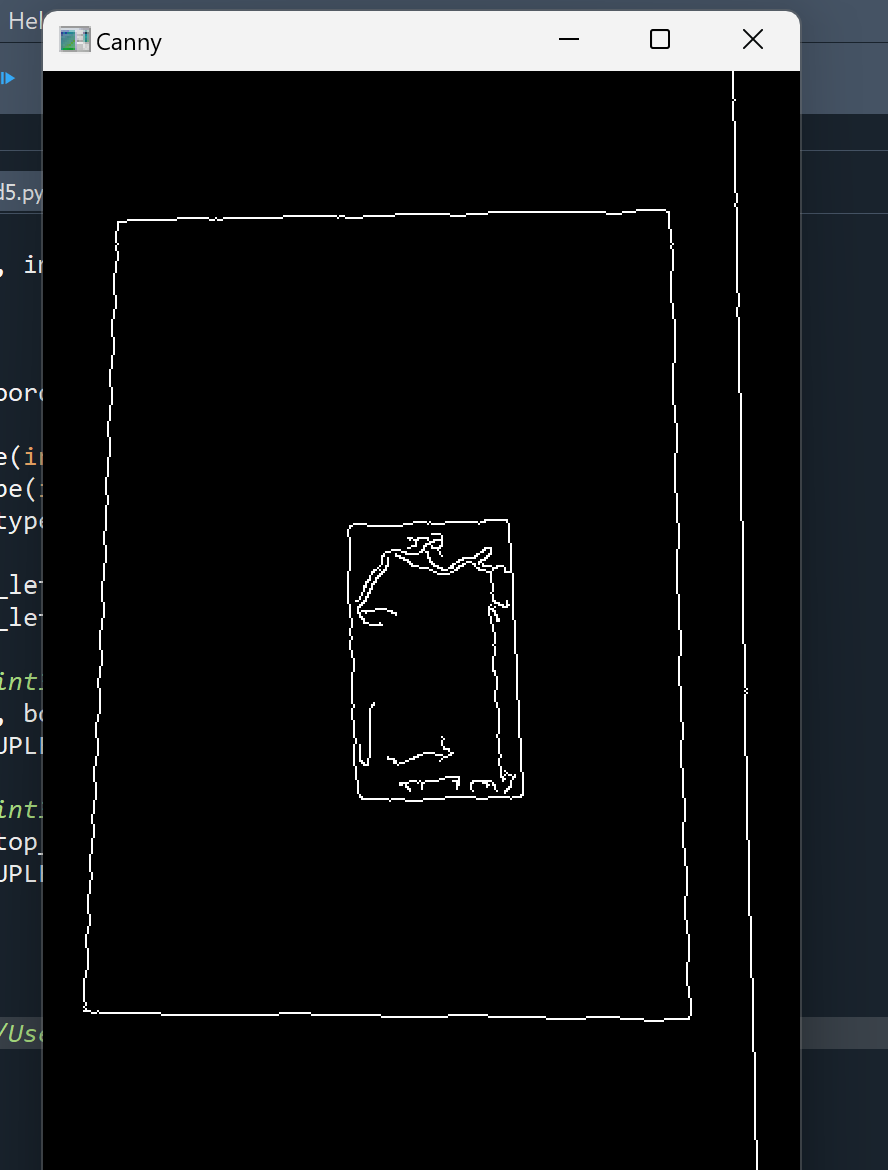
\includegraphics[width=0.65\linewidth]{nesne-2-siyah-beyaz}
			\caption*{Şekil-15 (c)}
		\end{minipage}\hfill
		\begin{minipage}[t]{0.470\linewidth}
			\centering
			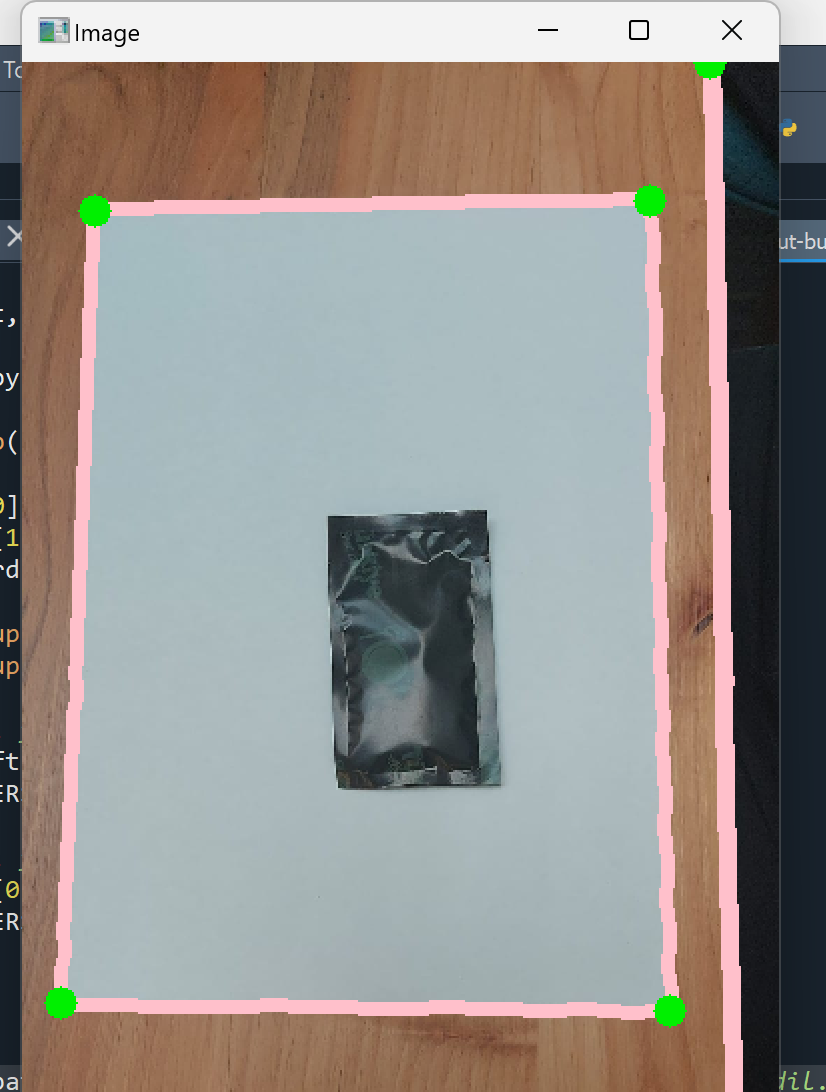
\includegraphics[width=0.65\linewidth]{nesne-2-a4}
			\caption*{Şekil-15 (d)}
		\end{minipage}
			\begin{minipage}[t]{0.470\linewidth}
			\centering
			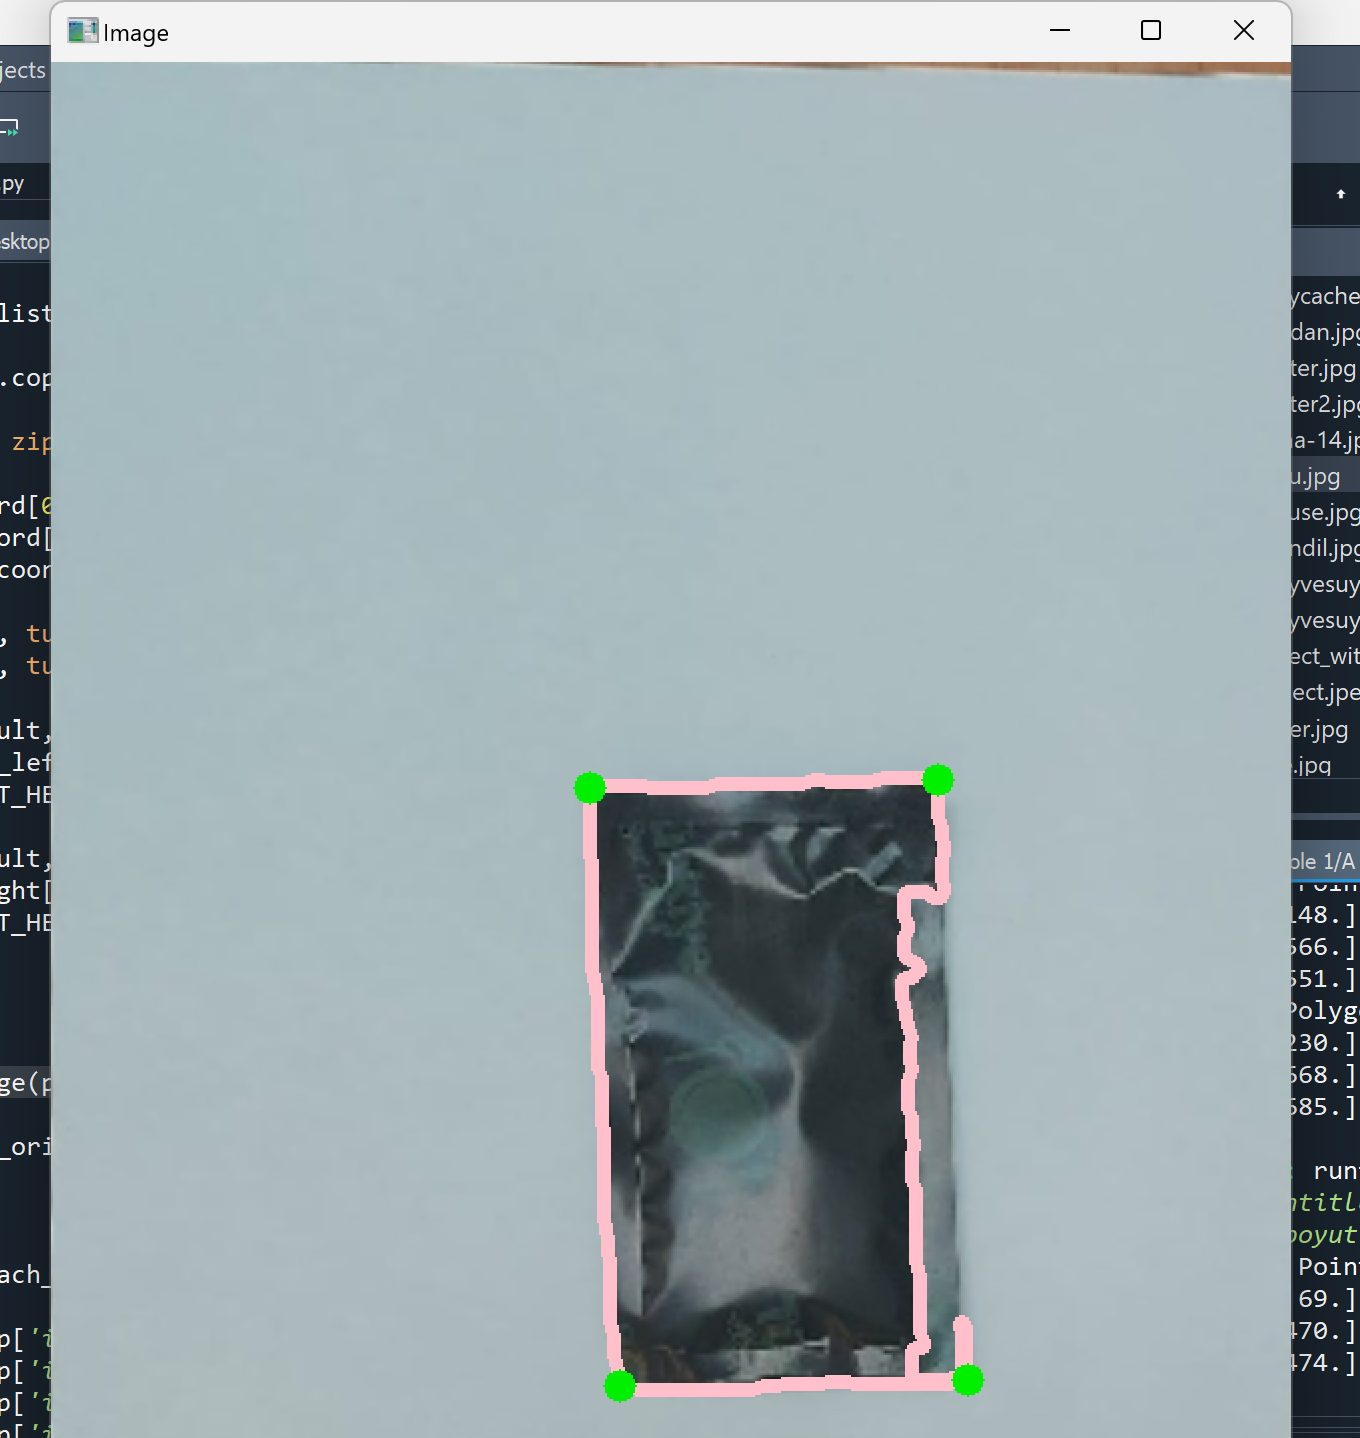
\includegraphics[width=0.65\linewidth]{nesne-2-cerceve}
			\caption*{Şekil-15 (e)}
		\end{minipage}\hfill
		\begin{minipage}[t]{0.470\linewidth}
			\centering
			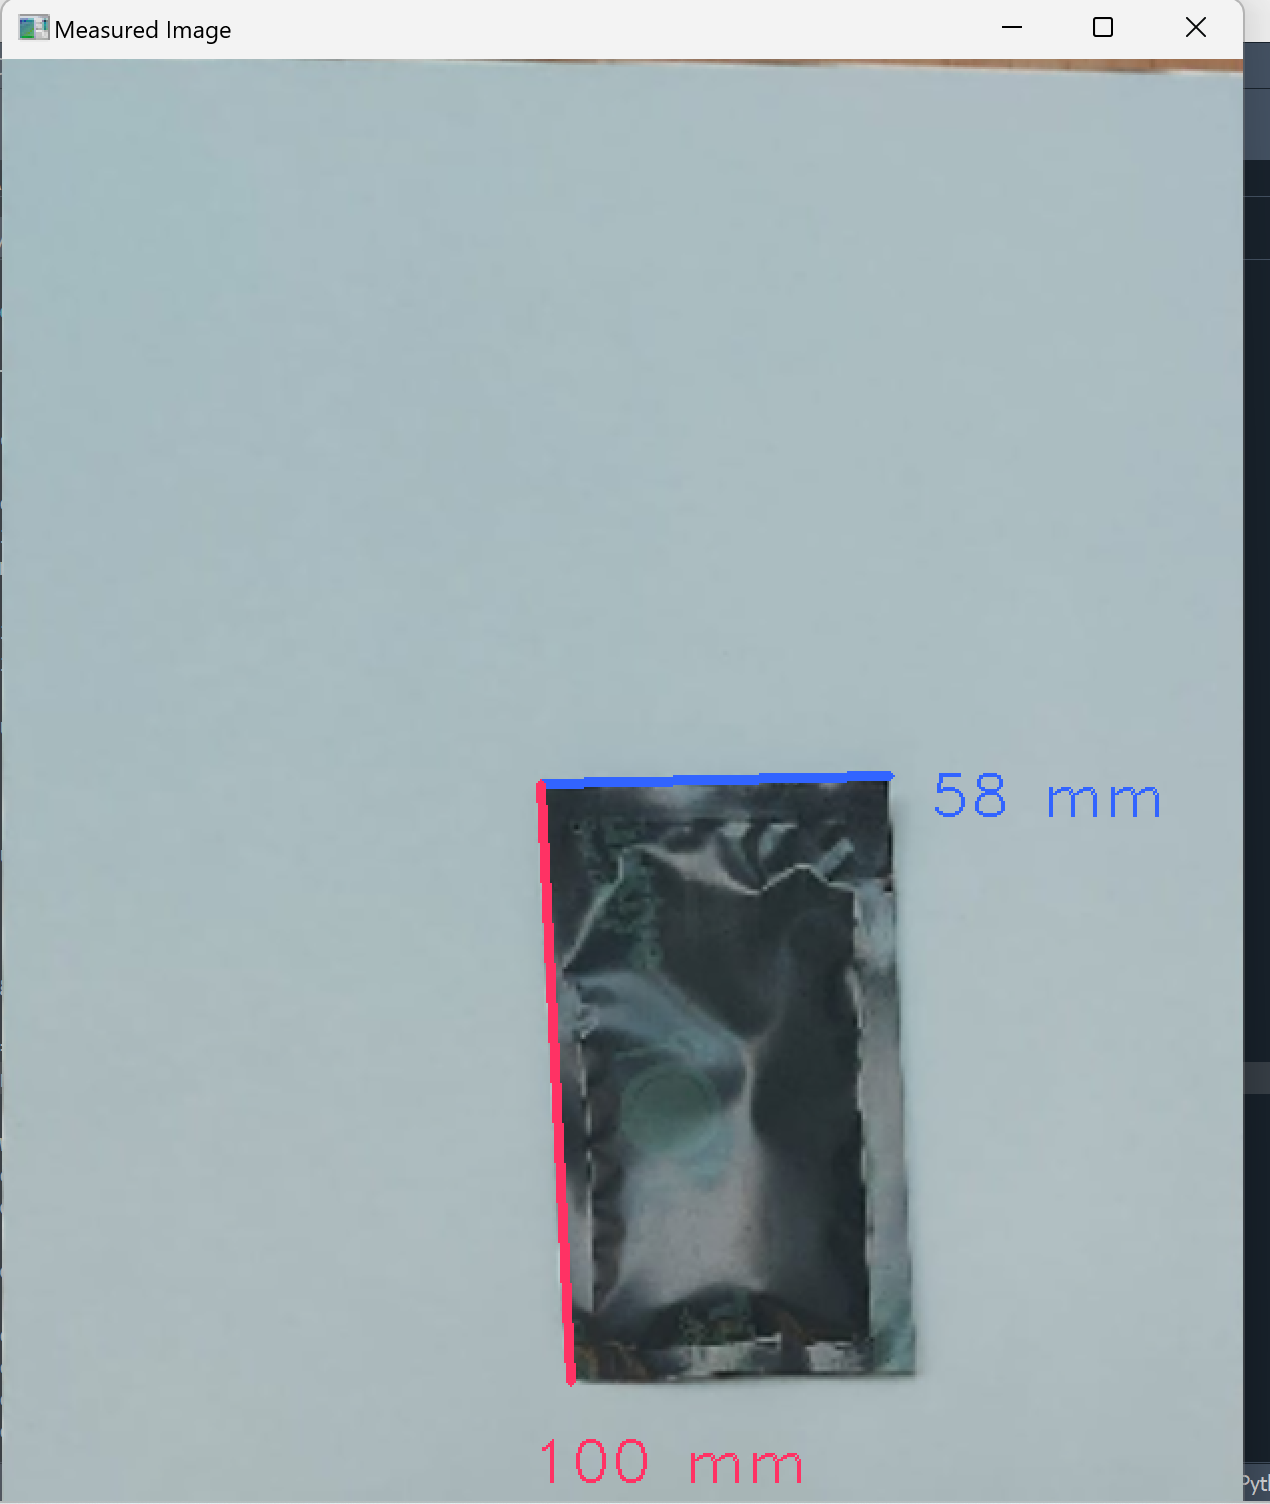
\includegraphics[width=0.65\linewidth]{boyut-bulma-sonuc-2}
			\caption*{Şekil-15 (f)}
		\end{minipage}
		\caption{ıslak mendil boyut bulma}
	\end{figure}
	\clearpage
	
		\section{Antropometri Nedir?}
	Antropometri tanımı, “insan” ve “ölçüm” anlamına gelen antropos ve metrikos Yunanca kelimelerine dayanmaktadır. İlgili alanlarda kullanılmak üzere insan vücudu parçalarının ölçüm verilerini organize etme, türetme ve analiz etme bilimidir.
	Antropometri, bireysel farklılıklara odaklanan ve çeşitli tasarım disiplinleri için önemli referanslar ve girdiler sağlayan ergonomi uygulamalarının hayati bir parçasıdır.Koltuklar, konsollar, ATM, araç iç hacimleri, cep telefonları, gamepadlar gibi insan vücudu ölçüleri içeren ürünler için ana tasarım çalışma konularından biridir. Mekanik tasarım yapacak mühendisler için de antropometri çalışmaları zaman zaman önem kazanmaktadır.\cite{antropometrinedir}
	
	Vücut ölçülerinin elde edilmesine yönelik, statik ve dinamik (fonksiyonel) antropometri olmak üzere iki farklı metot geliştirilmiştir.
	
	\subsection{Statik antropometri}İnsanların statik duruş ve oturuşlarında ölçülen boyutları ele alan bir uğraş alanıdır. Antropometrik ölçüler ayakta durma ve düz bir zeminde oturma durumlarına bağlı olarak özel aletlerin kullanımıyla alınmakta ve farklı ergonomik tasarımlarda kullanılmaktadır.Statik boyutlar, dirsek ve bilek arası ölçümler ile eklem merkezleri arasında ölçümler gibi insan iskeleti boyutları yanı sıra baş çevresi, cilt yüzeyi çevre ölçüleri gibi dış hat boyutlarını içermektedir.Çeşitli yaş gruplarındaki okul çocuklarının oturacağı sıraların boyutlarını saptamanın yanı sıra, bir gaz maskesinin yüz ölçülerine uygun bir şekilde ve boyutlarda imali için ihtiyaç duyulan antropometri ölçümler de statik antropometri yaklaşımı ile elde edilir.
	\subsection{Dinamik Antropometri}
	Endüstri ve iş ortamında iş görenler sürekli devinim hâlindedirler. Bir iş gören işini yaparken çeşitli yönlere uzanması, kol, bacak ve gövdesini değişik boyutlarda ve devamlı hareket ettirmesi nedeni ile çeşitli dinamik ölçülerin bilinmesine ihtiyaç duyulur. Fonksiyonel antropometri olarak da bilinen dinamik antropometri yaklaşımı ile elde edilen boyutlar, bazı fiziksel aktivitelerde bulunan insan vücudundan belli şartlar altında elde edilirler. İnsanların ayakta dururken ya da otururken çevrelerindeki malzemelere, kontrol sistemlerine ve çeşitli işlem noktalarına uzanabilmeleri için; eğilme, uzanma ve dönme gibi hareketlerinin hudutlarını ölçmek de iş düzeni ve insan-tezgâh, insan-makine gibi arakesitlerin tasarımında optimizasyon açısından önemlidir. Ancak çalışma ortamında insanların, sekreterin masasında bulunan telefona erişmesi, masanın çekmecesinden kâğıt almak için eğilmesi örneklerinde olduğu gibi, hareketlerde bulunmaları nedeniyle çeşitli dinamik boyutların ölçülmesine ihtiyaç duyulmuştur. İnsanların ayakta dururken ya da otururken çevrelerindeki malzemelere, kontrol araçlarına ve çeşitli işlem noktalarına eğilme, dönme, uzanma gibi hareketlerle erişebilecekleri sınırlar dinamik antropometri ile ölçülür.
	
	
	\subsection{Insan Bedeninde Altın Oran}
	
	İnsan vücudunda altın orana verilebilecek ilk örnek, göbek ile ayak arasındaki mesafe bir birim olarak kabul edildiğinde, insan boyunun $1,618'$e denk gelmesidir. Bunun dışında vücudumuzda yer alan diğer bazı altın oranlar şöyledir:
	
	\begin{itemize}
		\item Parmak ucu ile dirsek arası / El bileği ile dirsek arası
		\item Omuz hizasından başucuna olan mesafe / Kafa boyu
		\item Göbek ile başucu arası mesafe / Omuz hizasından başucuna olan mesafe
		\item Göbek ile diz arası / Diz ile ayakucu arası mesafe
	\end{itemize}
	
	Altın oran ile uyumlu tüm yapıların insan gözüne estetik açıdan ve uzunlukların birbirlerine uyumu açısından en güzel algılanan yapılar olduğu ve tercih sebebi olduğu gösterilmiştir. Altın oran parçalar veya uzuvlar arasında içsel bir uyum ve güzelliği bulundurur. Bu orana sahip bütünün tüm öğeleri insan gözüne çekici, estetik ve güzel gelmektedir. Altın orana diğer bir örnek ise Fibonacci dizisine tam bir uygunluk gösteren insan elidir. Parmaklarımız üç boğumludur. Parmağın tam boyunun ilk iki boğuma oranı altın oranı verir (başparmak dışındaki parmaklar için). Ayrıca orta parmağın serçe parmağına oranında da altın oran olduğunu fark edilebilmektedir.
	
	\begin{figure}[!h]
		\centering
		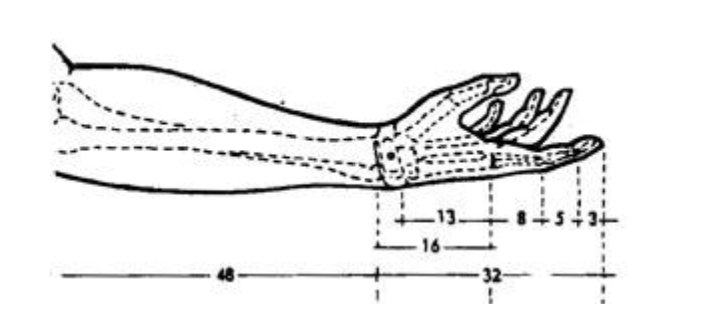
\includegraphics[ width=\textwidth]{el}
		\caption{el\cite{}}
		
	\end{figure}
	
	
	
	Şekilde her ardışık bölüm arasındaki oran altın oran sabiti olan $0,618\ldots$ sayısıdır. Ayrıca her bölüm 2, 3, 5, 8'e yani ardışık Fibonacci sayılarına karşılık gelmektedir.
	
	\begin{figure}[!h]
		\centering
		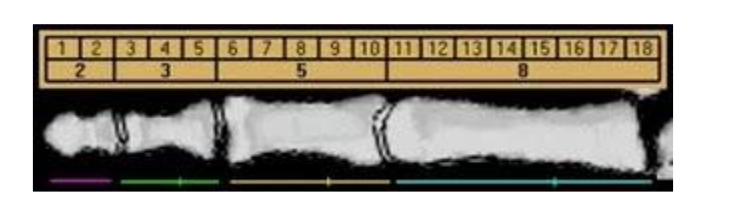
\includegraphics[width=0.70\textwidth]{parmak}
		\caption{Parmak Uçlarındaki Altın Oranı Gösteren Çizgiler}
	\end{figure}
	
	Şekildeki pembe, yeşil, sarı ve mavi çizgiler altın oranı göstermektedir.\cite{sencer2012gencc}
	
	
	\section{Projeler}
	Eli referans olarak alıp meyvelerin gerçek boyutunun bulunabilmesi için ilk olarak doğru bir şekilde el ölçümü yapılmalıdır.
	
	\begin{figure}[!h]
		\centering
		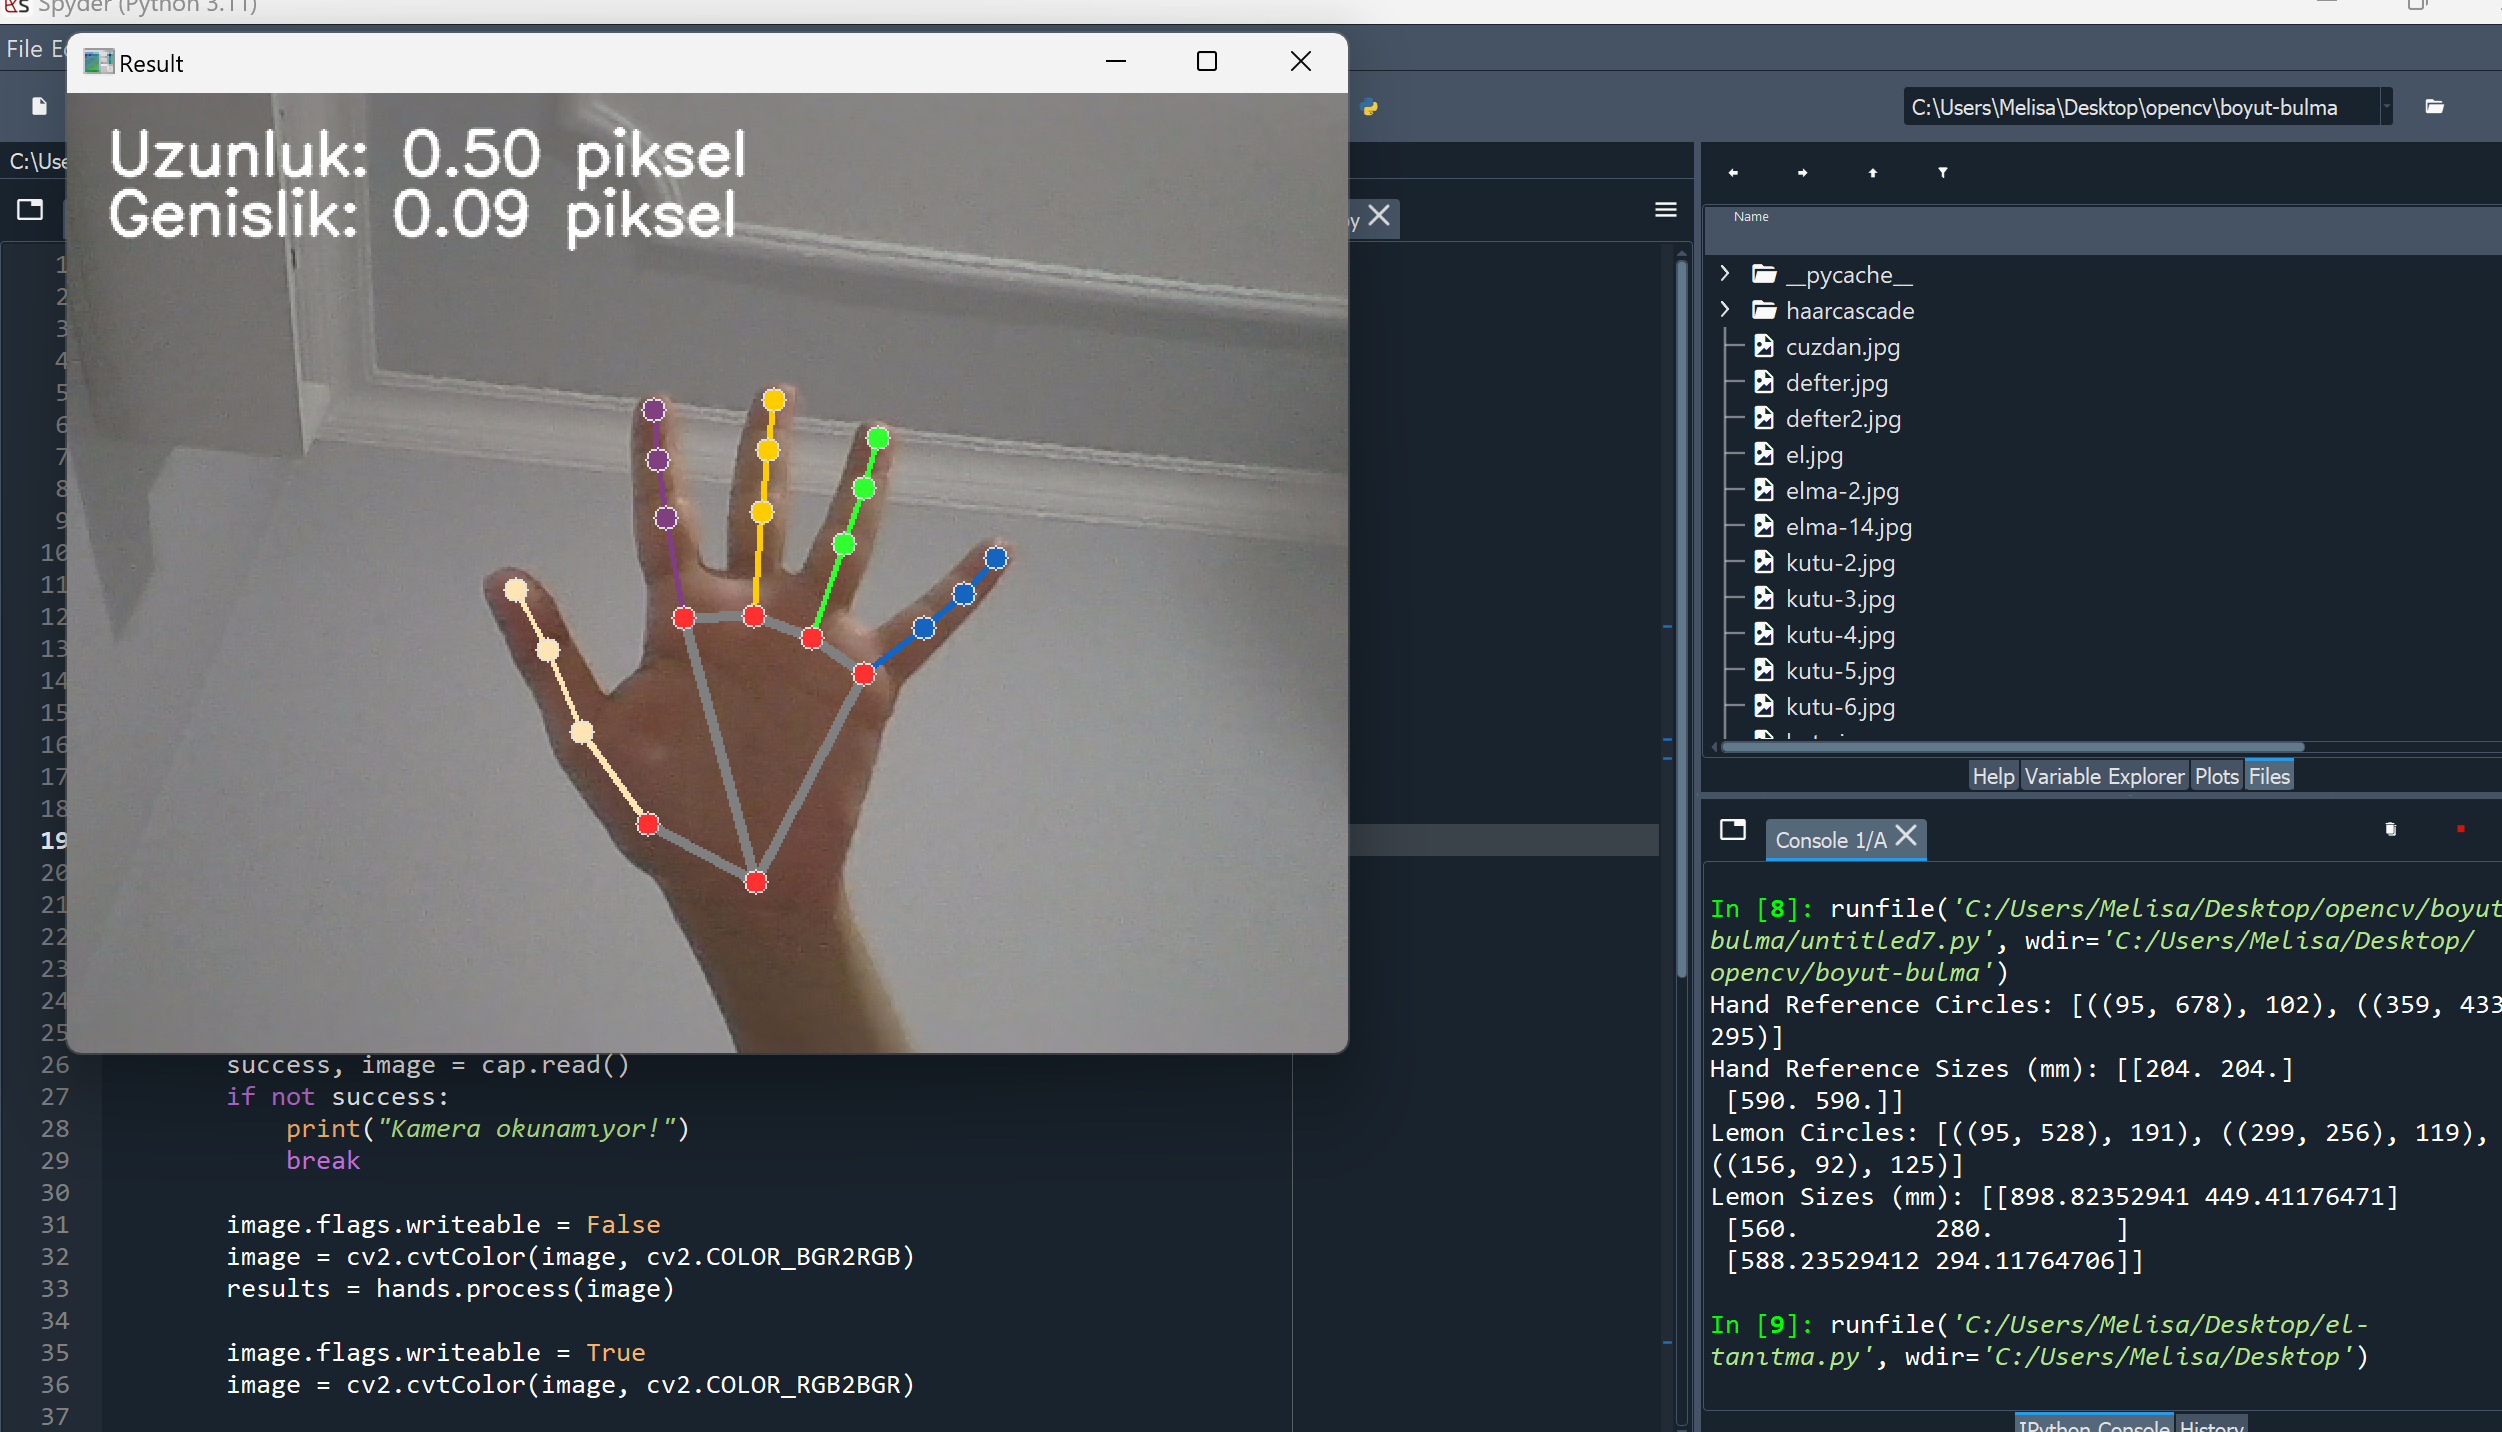
\includegraphics[width=\textwidth]{el-boyut}
		\caption{Eklemler yardımı ile el şekli çıkartımı}
		\label{el}
	\end{figure}
	
	Şekil -\ref{el} de orta parmağın en üst kısmından avcun en alt noktası arasındaki uzaklık ölçümü ile elin uzunluğu yaklaşık olarak bulunmuştur. Baş parmağın üst kısmından serçe parmağın en altındaki nokta arasındakı uzaklıktan elin genişliğinin yaklaşık değeri bulunmuştur.
	
	\begin{figure}[!h]
		\centering
		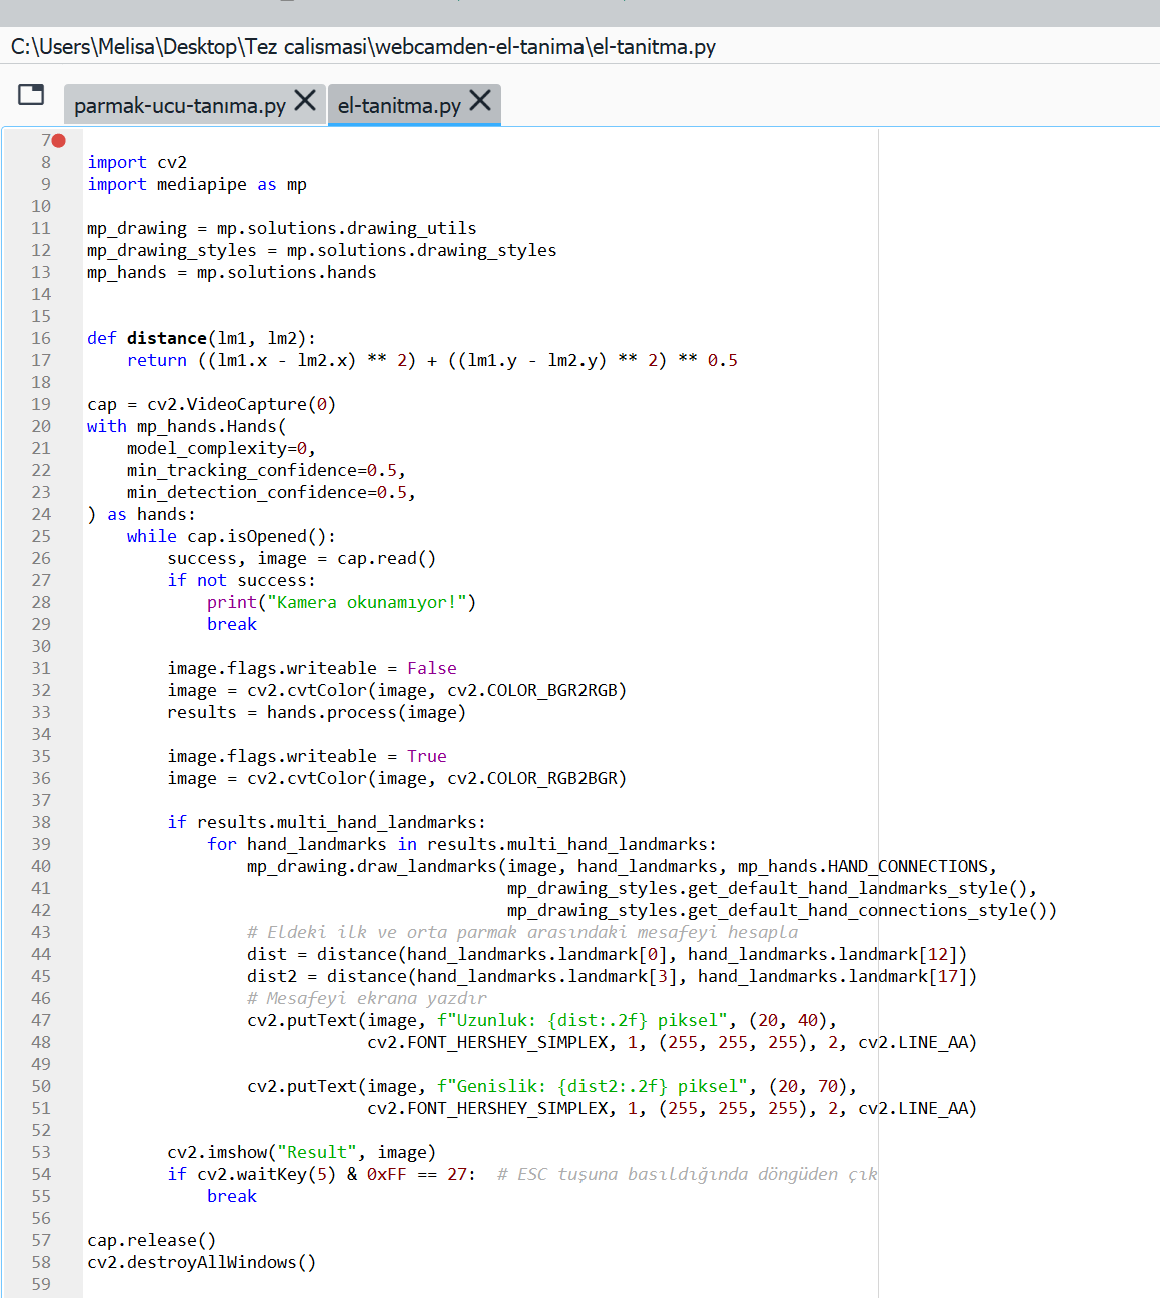
\includegraphics[width=0.65\textwidth]{el boyut kod2}
		\caption{El Şeklini Çıkaran Kod}
	\end{figure}
	
	\begin{figure}[!h]
		\centering
		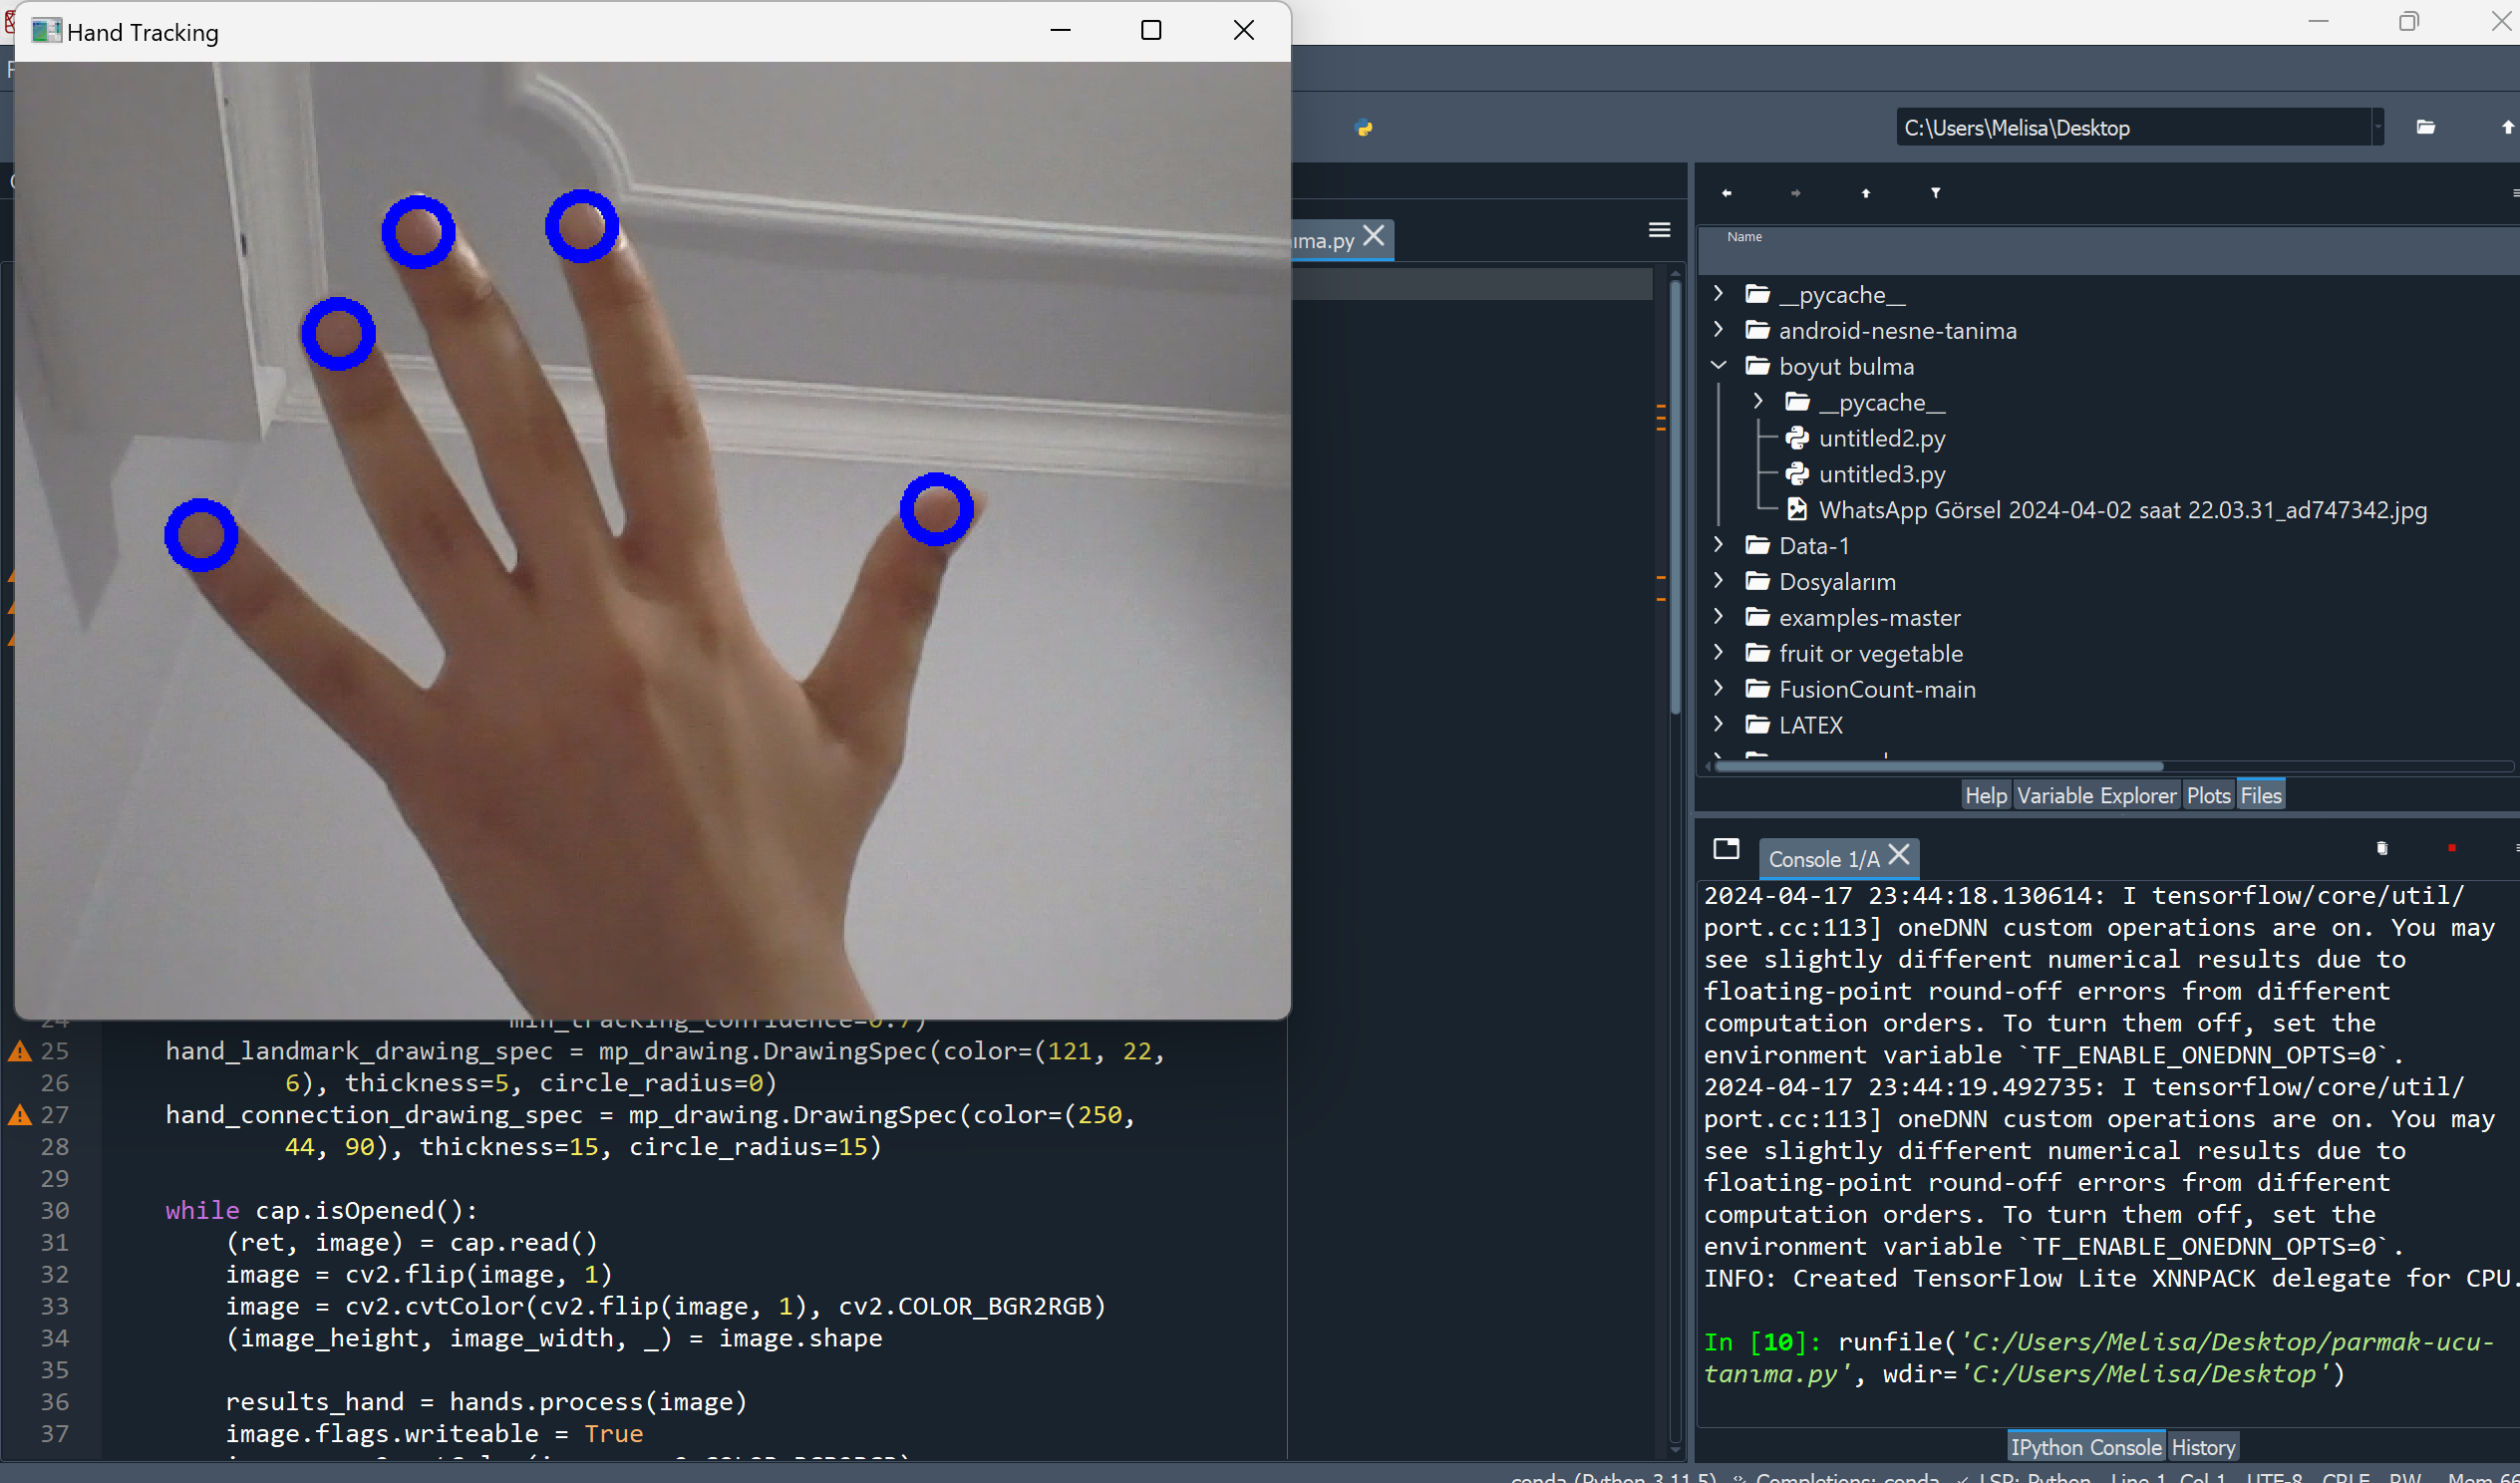
\includegraphics[width=\textwidth]{tırnak}
		\caption{Parmak Uçlarının bulunması}
		\label{tırnak}
	\end{figure}
	
	Şekil -\ref{tırnak} da parmak uçları bulunarak tırnaklar belirlenmiştir.
	\begin{figure}[!h]
		\centering
		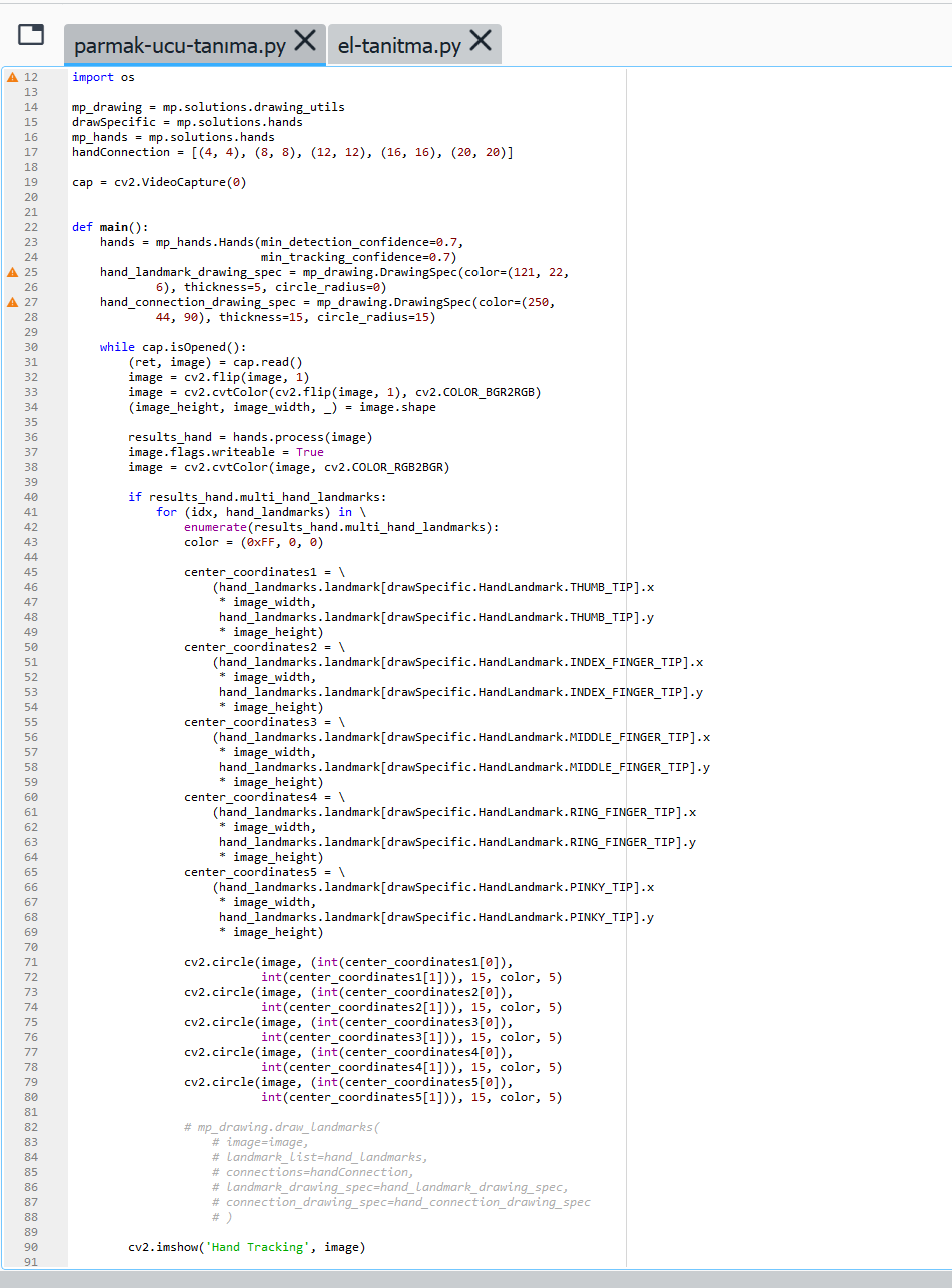
\includegraphics[width=\textwidth]{tırnak-kod2}
		\caption{Parmak Uçlarının bulunduğu kod}
	\end{figure}
	
	\begin{figure}[!h]
		\centering
		\begin{minipage}{0.45\textwidth} % Sol fotoğraf için minipage
			\centering
			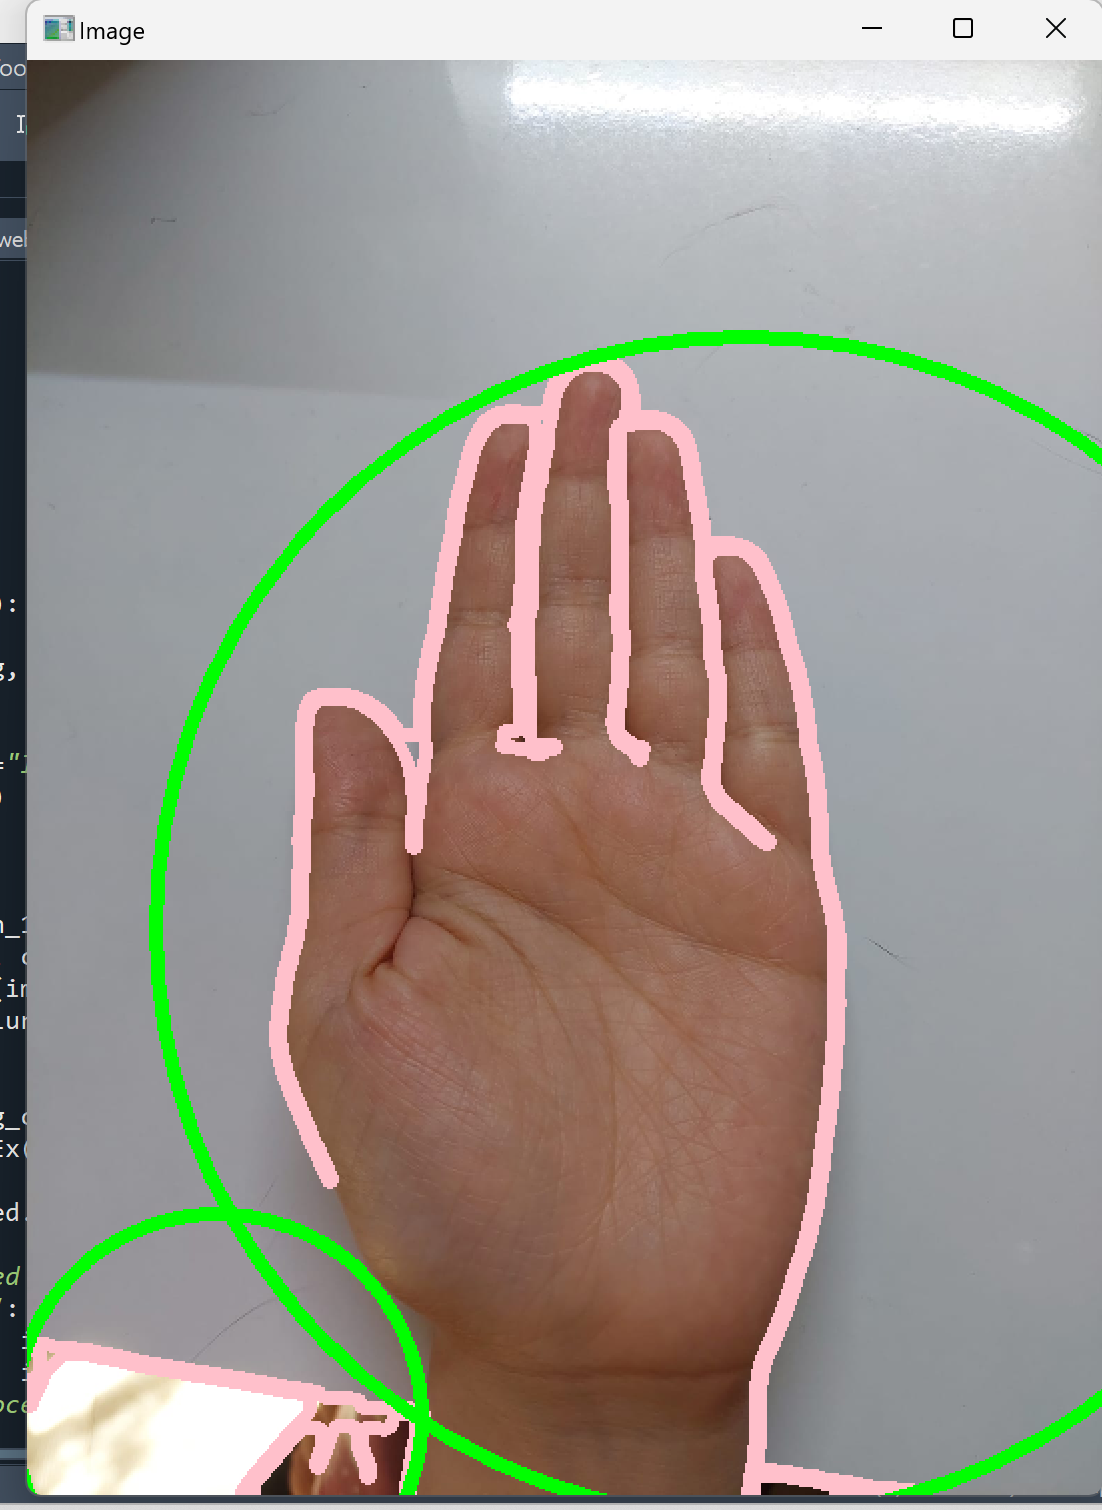
\includegraphics[width=\linewidth]{hatalı-el}
			\label{boyutbulma1}
			\caption*{Şekil-22 (a)}
		\end{minipage}%
		\hfill % Yatay boşluk
		\begin{minipage}{0.45\textwidth} % Sağ fotoğraf için minipage
			\centering
			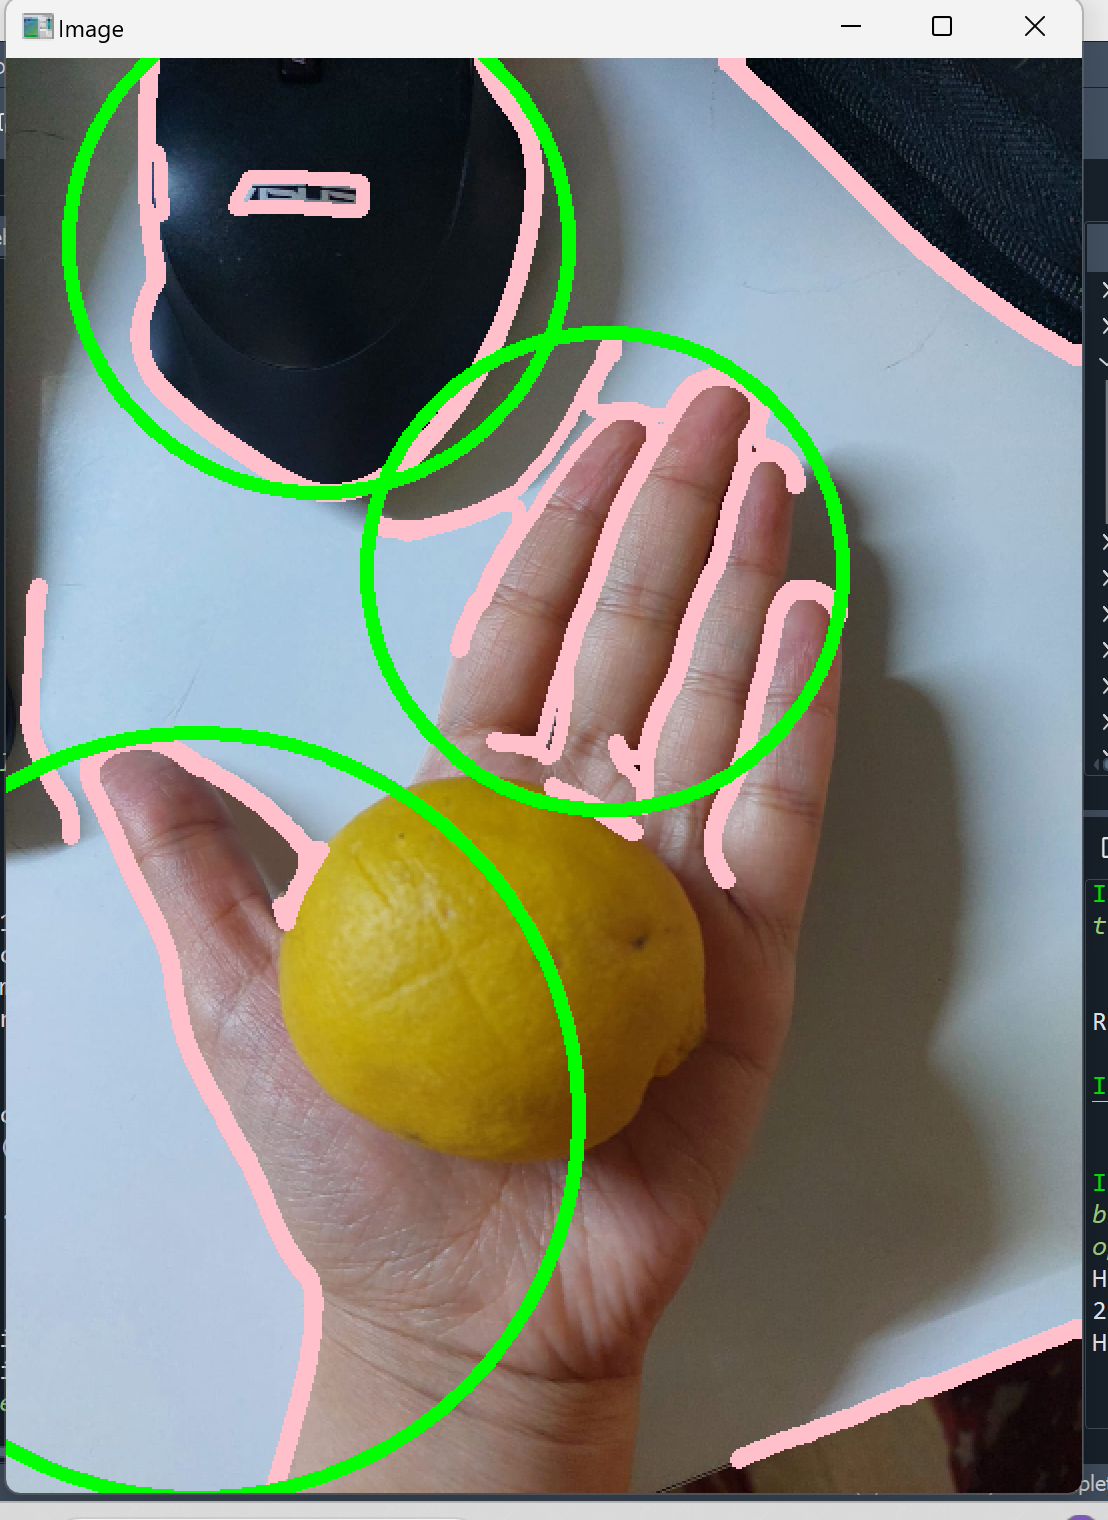
\includegraphics[width=\linewidth]{hatalı-olcum-1}
			\label{boyutbulma2}
			\caption*{Şekil-22 (b)}
		\end{minipage}
		
		\vspace{1cm} % Dikey boşluk
		
		\begin{minipage}{\textwidth} % Alt fotoğraf için minipage
			\centering
			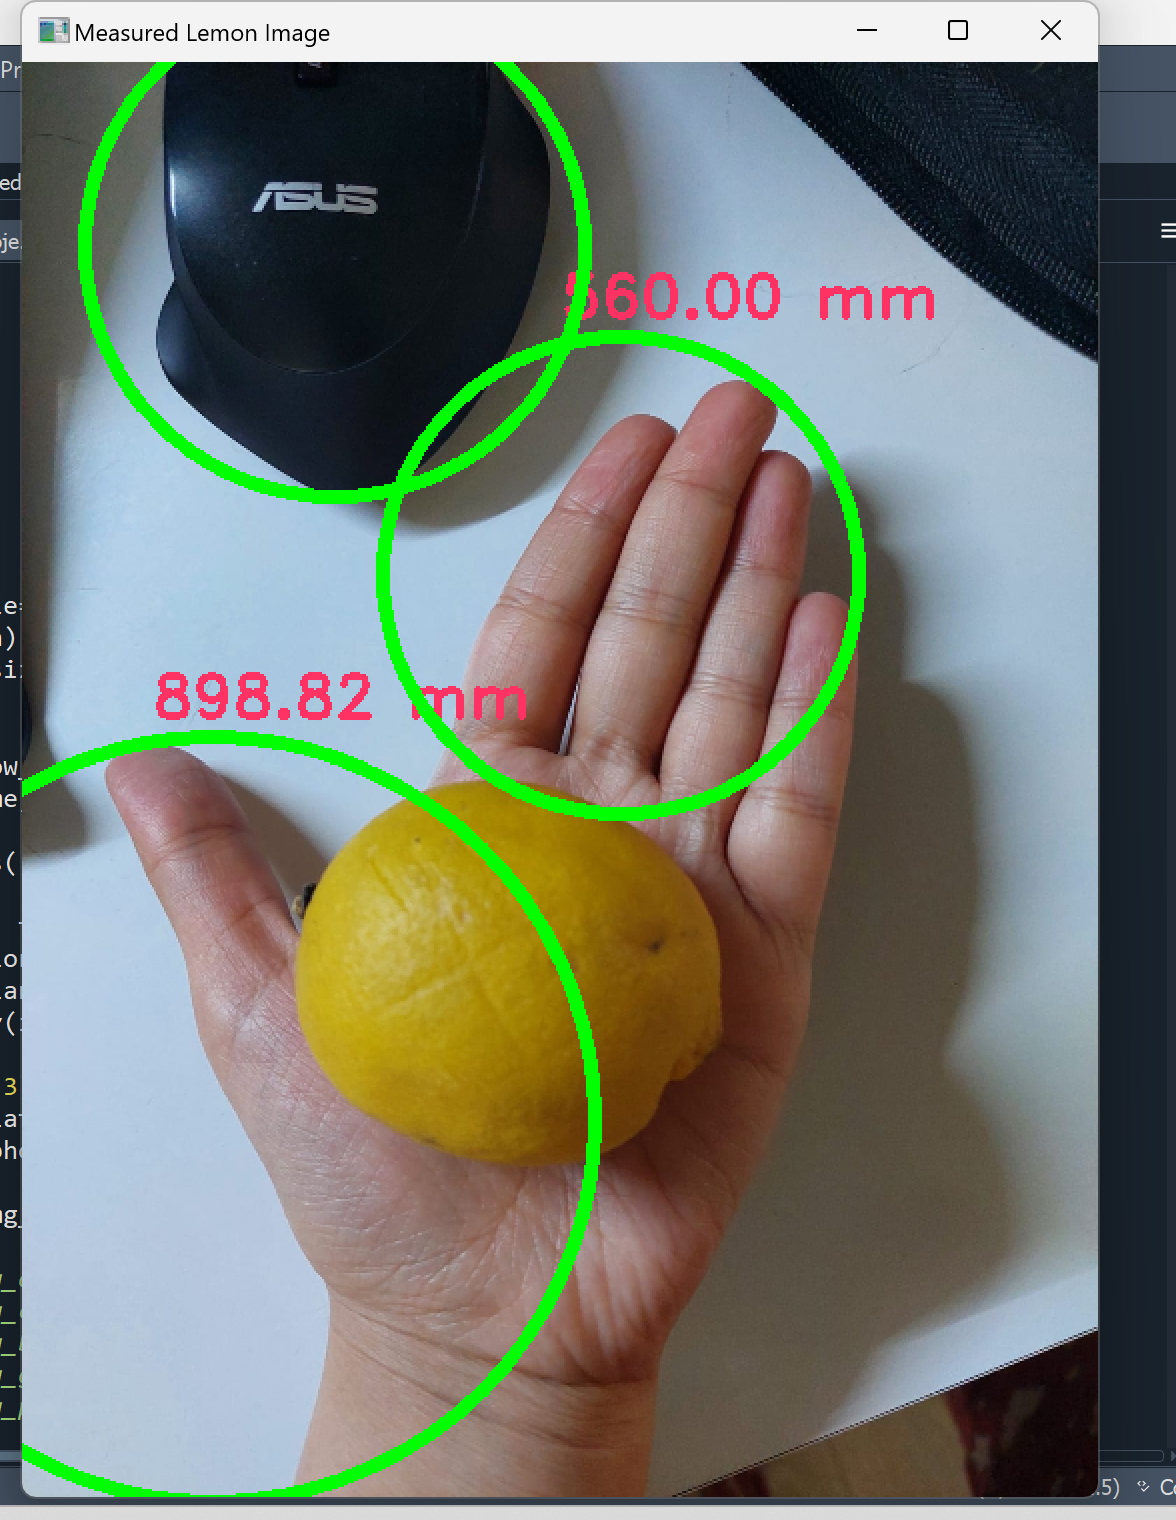
\includegraphics[width=0.5\linewidth]{hatalı-olcum-2}
			\caption*{Şekil-22 (c)}
			\label{boyutbulma3}
		\end{minipage}
		
		\caption{Hatalı Nesne Ölçümü} % Üç fotoğrafın altına tek açıklama
		\label{el-nesne-boyutlar}
	\end{figure}
	
	
	Yararlanılan diğer kaynaklar\cite{youtube}\cite{stackoverflow}
	\bibliographystyle{plain}
	\bibliography{kaynak}
\end{document}